\باب{مخروطی حصے، منحنی مقدار معلوم اور قطبی محدد}

\جزوحصہء{جائزہ}
حرکت پر غور احصاء کی مدد سے کیا جا سکتا ہے۔ اس حصہ میں ہم وقت کے ساتھ ایک ذرے کے بدلتے مقام پر غور کریں گے۔ ہم  مخروطی حصوں کی مساوات سے شروع کرتے ہیں چونکہ بالعکس مربع قوت کی بنا سیارے، مصنوعی سیارے، اور دیگر اجسام  مخروطی راہ پر حرکت کرتے ہیں۔ اگر ہمیں معلوم ہو کہ ایک جسم مخروطی راہ پر حرکت کر رہا ہے  تب ہم اس کی رفتار اور اس پر عمل کرنے والی قوت دریافت کر سکتے ہیں۔  قطبی محدد سیاروں کی حرکت پر غور کو بہت آسان بناتا ہے لہٰذا ہم اس نئے محدد میں منحنیات، تفرق اور تکمل پر بھی غور کریں گے۔

\حصہ{مخروطی حصے اور دو قدری مساواتیں}\شناخت{حصہ_مخروط_حصے_دو_قدری_مساواتیں}
اس حصہ میں دکھایا جائے گا کہ مخروطی حصوں کو کس  طرح محددی سطح پر بطور دو قدری مساوات پیش کیا جاتا ہے۔ دوہرے مخروط کو سطح سے کاٹ کر مخروطی منحنیات پیدا کی جاتی ہیں اور اسی کی بنا مخروطی حصہ کی اصطلاح پیدا ہوئی۔

\جزوحصہء{دائرہ}
\ابتدا{تعریف}
ایک مستوی میں رہتے ہوئے اس مستوی میں کسی مقررہ نقطہ سے مستقل فاصلے پر تمام نقطوں کے سلسلہ کو \اصطلاح{دائرہ}\فرہنگ{دائرہ}\حاشیہب{circle}\فرہنگ{circle} کہتے ہیں۔ اس مقررہ نقطہ کو دائرے کا \اصطلاح{مرکز}\فرہنگ{مرکز}\حاشیہب{center}\فرہنگ{center} کہتے ہیں جبکہ اس مستقل فاصلہ کو \اصطلاح{رداس}\فرہنگ{رداس}\حاشیہب{radius}\فرہنگ{radius} کہتے ہیں۔ 
\انتہا{تعریف}
 
 دائرے کے معیاری مساوات جنہیں حصہ \حوالہ{حصہ_ابتدا_ترسیم_کی_منتقلی} میں فاصلہ کی مساوات \عددی{d=\sqrt{(x_2-x_1)^2+(y_2-y_1)^2}} سے اخذ کیا گیا درج ذیل ہیں۔
\begin{align*}
x^2+y^2&=a^2&&\text{\RL{رداس \عددی{a} اور مرکز \عددی{(0,0)}}}\\
(x-h)^2+(y-k)^2&=a^2&&\text{\RL{رداس \عددی{a} اور مرکز \عددی{(h,k)}}}
\end{align*}

\جزوحصہء{قطع مکافی}
\ابتدا{تعریف}
ایک سطح میں رہتے ہوئے کسی مقررہ سیدھی لکیر اور مقررہ نقطہ (جو اس مقررہ سیدھی لکیر پر نہیں پایا جاتا ہو) سے مستقل فاصلہ پر پائے جانے والے تمام نقطوں کے سلسلہ کو \اصطلاح{قطع مکافی}\فرہنگ{قطع مکافی}\حاشیہب{parabola}\فرہنگ{parabola} کہتے ہیں۔مقررہ نقطے کو قطع مکافی کا \عددی{ماسکہ}\فرہنگ{ماسکہ}\حاشیہب{focus}\فرہنگ{focus} کہتے ہیں جبکہ مقررہ لکیر کو \اصطلاح{ناظمہ}\فرہنگ{ناظمہ}\حاشیہب{directrix}\فرہنگ{directrix} کہتے ہیں۔ 
\انتہا{تعریف}
%==============

جب ماسکہ کسی محددی محور پر ہو اور ناظمہ اس محددی محور کے متوازی ہو تب قطع مکافی کی مساوات سادہ ترین ہوتی ہے۔مثال کے طور پر، فرض کریں کہ ماسکہ \عددی{y} محور پر نقطہ \عددی{F(0,p)} پر پایا جاتا ہے اور لکیر \عددی{y=-p} ناظمہ (شکل \حوالہ{شکل_مخروط_قطع_مکافی_الف})  ہے۔ یوں شکل \حوالہ{شکل_مخروط_قطع_مکافی_الف} میں نقطہ \عددی{N(x,y)} صرف اور صرف اس صورت اس قطع مکافی پر پایا جائے گا جب \عددی{NF=NQ} ہو۔ فاصلہ کے کلیہ سے
\begin{align*}
NF&=\sqrt{(x-0)^2+(y-p)^2}=\sqrt{x^2+(y-p)^2}\\
NQ&=\sqrt{(x-x)^2+(y-(-p))^2}=\sqrt{(y+p)^2}
\end{align*}
لکھا جا سکتا ہے۔ ان مساوات کو ایک دوسرے کے برابر پر کر کے حل کرتے ہوئے درج ذیل حاصل ہو گا۔
\begin{align}\label{مساوات_مخروط_قطع_مکافی_معیاری_الف}
y&=\frac{x^2}{4p}\quad \implies \quad x^2=4py&&\text{\RL{معیاری روپ}}
\end{align}
اس مساوات سے قطع مکافی کی \عددی{y} محور کے لحاظ سے تشاکلی واضح ہے۔ ہم کہتے ہیں کہ محور \عددی{y} اس قطع مکافی کا محور تشاکلی ہے جس کو عموماً چھوٹا کر کے صرف \اصطلاح{محور}\فرہنگ{محور}\حاشیہب{axis}\فرہنگ{axis} پکارا جاتا ہے۔

وہ نقطہ جس پر قطع مکافی اپنے محور کو قطع کرتا ہو \اصطلاح{راس}\فرہنگ{راس}\حاشیہب{vertex}\فرہنگ{vertex} کہلاتا ہے۔ قطع مکافی \عددی{x^2=4py} کا راس مبدا پر پایا جاتا ہے (شکل \حوالہ{شکل_مخروط_قطع_مکافی_الف})۔ مثبت عدد \عددی{p} کو قطع مکافی کا \اصطلاح{طول ماسکہ}\فرہنگ{ماسکہ!طول}\حاشیہب{focal length}\فرہنگ{focal!length} کہتے ہیں۔
\begin{figure}
\centering
\begin{minipage}{0.45\textwidth}
\centering
\begin{tikzpicture}[declare function={f(\x)=1/4*\x^2;}]
\pgfmathsetmacro{\a}{1.5}
\pgfmathsetmacro{\b}{f(\a)}
\begin{axis}[clip=false,small,axis lines=middle, xtick={\empty},ytick={\empty}, enlargelimits=true,ymin=-1.25, xlabel={$x$},ylabel={$y$}, xlabel style={at={(current axis.right of origin)},anchor=west},ylabel style={at={(current axis.above origin)},anchor=south}]
\addplot[domain=-2.5:2.5]{f(x)}node[pos=0.1,left]{$x^2=4py$};
\addplot[]plot coordinates {(0,1)}node[circ]{}node[left]{ماسکہ}node[above right]{$F(0,p)$};
\addplot[]plot coordinates {(0,1)(\a,\b)}node[circ]{}node[right]{$N(x,y)$};
\addplot[]plot coordinates {(-2.5,-1)(2.5,-1)}node[right]{$L$}node[pos=0.25,above]{ناظمہ}node[pos=0.25,yshift={-0.5ex},below]{$y=-p$};
\addplot[dashed] plot coordinates {(\a,\b)(\a,-1)}node[circ]{}node[below]{$Q(x,-p)$};
\addplot[]plot coordinates {(0,0.5)}node[left]{$p$};
\addplot[]plot coordinates {(0,-0.5)}node[left]{$p$};
\addplot[]plot coordinates {(0,0)}node[circ]{}node[below right]{راس};
\end{axis}
\end{tikzpicture}
\caption{قطع مکافی \عددی{x^2=4py}؛ راس کا فاصل ماسکہ اور ناظمہ سے ایک جیسا ہے۔}
\label{شکل_مخروط_قطع_مکافی_الف}
\end{minipage}\hfill
\begin{minipage}{0.45\textwidth}
\centering
\begin{tikzpicture}[declare function={f(\x)=-1/4*\x^2;}]
\pgfmathsetmacro{\a}{1.5}
\pgfmathsetmacro{\b}{f(\a)}
\begin{axis}[clip=false,small,axis lines=middle,xtick={\empty},ytick={\empty},enlargelimits=true,ymin=-1.25,xlabel={$x$},ylabel={$y$},xlabel style={at={(current axis.right of origin)},anchor=west},ylabel style={at={(current axis.above origin)},anchor=south}]
\addplot[domain=-2.5:2.5]{f(x)}node[pos=0.2,left]{$x^2=-4py$};
\addplot[]plot coordinates {(0,-1)}node[circ]{}node[left]{ماسکہ}node[right]{$F(0,-p)$};
\addplot[]plot coordinates {(-2.5,1)(2.5,1)}node[right]{$L$}node[pos=0.25,above]{ناظمہ}node[pos=0.25,yshift={-0.5ex},below]{$y=p$};
\addplot[]plot coordinates {(0,0)}node[circ]{}node[above left]{\RL{راس مبدا پر ہے}};
\end{axis}
\end{tikzpicture}
\caption{قطع مکافی \عددی{x^2=-4py}}
\label{شکل_مخروط_قطع_مکافی_ب}
\end{minipage}
\end{figure}

اگر قطع مکافی نیچے رخ کھلتا ہو اور اس کا ماسکہ \عددی{(0,-p)} جبکہ ناظمہ لکیر \عددی{y=p} ہو تب مساوات \حوالہ{مساوات_مخروط_قطع_مکافی_معیاری_الف} درج ذیل روپ اختیار کرے گی (شکل \حوالہ{شکل_مخروط_قطع_مکافی_ب})۔
\begin{align*}
y=-\frac{x^2}{4p}\quad \implies \quad x^2=-4py
\end{align*}
ہم اسی طرح کے مساوات ہم دائیں اور بائیں کھلنے والے قطع مکافی کے لئے حاصل کر سکتے ہیں (جدول \حوالہ{جدول_مخروط_کھلنے_کی_سمت} اور شکل \حوالہ{شکل_مخروط_قطع+مکافی_بائیں_دائیں})۔

\begin{table}
\caption{مبدا پر راس والے قطع مکافی کے معیاری مساوات (\عددی{p>0})}
\label{جدول_مخروط_کھلنے_کی_سمت}
\centering
\begin{tabular}{LCLCC}
\text{مساوات}&\text{ماسکہ}&\text{ناظمہ}&\text{محور}&\text{\RL{کھلنے کا رخ}}\\
\toprule
x^2=4py&(0,p)&y=-p&\text{\عددی{y} محور}&\text{اوپر}\\
x^2=-4py&(0,-p)&y=p&\text{\عددی{y} محور}&\text{نیچے}\\
y^2=4px&(p,0)&x=-p&\text{\عددی{x} محور}&\text{دائیں}\\
y^2=-4px&(-p,0)&x=p&\text{\عددی{x} محور}&\text{بائیں}
\end{tabular}
\end{table}

\begin{figure}
\centering
\begin{subfigure}{0.45\textwidth}
\centering
\begin{tikzpicture}[declare function={fp(\x)=sqrt(4*\x);fn(\x)=-sqrt(4*\x);}]
\begin{axis}[clip=false,small,axis lines=middle,xlabel={$x$},ylabel={$y$},xtick={\empty},ytick={\empty},xlabel style={at={(current axis.right of origin)},anchor=west},ylabel style={at={(current axis.above origin)},anchor=south},xmin=-1.25]
\addplot[domain=0:0.2]{fp(x)};
\addplot[domain=0:0.2]{fn(x)};
\addplot[domain=0.2:2]{fp(x)}node[pos=0.75,above left]{$y^2=4px$};
\addplot[domain=0.2:2]{fn(x)};
\addplot[]plot coordinates {(1,0)}node[circ]{}node[above]{ماسکہ}node[below]{$F(p,0)$};
\addplot[]plot coordinates {(0,0)}node[circ]{}node[above left]{راس};
\addplot[]plot coordinates {(-1,-3)(-1,3)}node[pos=0.8,left]{ناظمہ}node[pos=0.8,below]{\scriptsize{$x=-p$}};
\end{axis}
\end{tikzpicture}
\end{subfigure}\hfill
\begin{subfigure}{0.45\textwidth}
\centering
\begin{tikzpicture}[declare function={fp(\x)=sqrt(4*\x);fn(\x)=-sqrt(4*\x);}]
\begin{axis}[clip=false,small,axis lines=middle,xlabel={$x$},ylabel={$y$},xtick={\empty},ytick={\empty},xlabel style={at={(current axis.right of origin)},anchor=west},ylabel style={at={(current axis.above origin)},anchor=south},xmax=1.25]
\addplot[domain=0:0.2]({-x},{fp(x)});
\addplot[domain=0:0.2]({-x},{fn(x)});
\addplot[domain=0.2:2]({-x},{fp(x)})node[pos=0.75,above right]{$y^2=-4px$};
\addplot[domain=0.2:2]({-x},{fn(x)});
\addplot[]plot coordinates {(-1,0)}node[circ]{}node[above]{ماسکہ}node[below]{$F(-p,0)$};
\addplot[]plot coordinates {(0,0)}node[circ]{}node[above right]{راس};
\addplot[]plot coordinates {(1,-3)(1,3)}node[pos=0.8,right]{ناظمہ}node[pos=0.8,below right]{\scriptsize{$x=p$}};
\end{axis}
\end{tikzpicture}
\end{subfigure}
\caption{قطع مکافی \عددی{y^2=4px} اور \عددی{y^2=-4px} کے ترسیمات۔}
\label{شکل_مخروط_قطع+مکافی_بائیں_دائیں}
\end{figure}

\ابتدا{مثال}
قطع مکافی \عددی{y^2=10x} کا ماسکہ اور ناظمہ تلاش کریں۔

حل:\quad
ہم معیاری مساوات \عددی{y^2=4px} میں \عددی{p} کی قیمت تلاش کرتے ہیں:
\begin{align*}
4p=10\quad \implies \quad p=\frac{10}{4}=\frac{5}{2}
\end{align*}
اس کے بعد ہم حاصل کردہ \عددی{p} کے لئے ماسکہ اور ناظمہ تلاش کرتے ہیں۔
\begin{align*}
(p,0)&=\big(\frac{5}{2},0\big)&&\text{ماسکہ}\\
x&=-p, \quad \quad x=-\frac{5}{2}&&\text{ناظمہ}
\end{align*}
\انتہا{مثال}
%=======================

جدول \حوالہ{جدول_مخروط_کھلنے_کی_سمت} کے کلیات پر حصہ \حوالہ{حصہ_ابتدا_ترسیم_کی_منتقلی} میں دیے گئے منتقلی کے کلیات لاگو کرتے ہوئے دیگر مقامات پر واقع قطع مکافی کے مساوات حاصل کئے جا سکتے ہیں۔

\جزوحصہء{ترخیم}
\ابتدا{تعریف}
ایک مستوی پر رہتے ہوئے، مستوی پر دو مقررہ نقطوں سے جن نقطوں کے فاصلوں کا مجموعہ مستقل ہو، ان کے سلسلہ کو \اصطلاح{ترخیم}\فرہنگ{ترخیم}\حاشیہب{ellipse}\فرہنگ{ellipse} کہتے ہیں۔ ان دو مقررہ نقطوں کو ترخیم کے \اصطلاح{ماسکے} کہتے ہیں (شکل \حوالہ{شکل_مخروط_ترخیم_کی_تعریف} اور شکل \حوالہ{شکل_مخروط_ترخیم_اہم_نقطے})۔
\انتہا{تعریف}
%================

ترخیم کو اس کی تعریف استعمال کرتے ہوئے بہت جلد ترسیم کیا جا سکتا ہے۔ مقررہ نقطوں \عددی{F_1} اور \عددی{F_2} پر ڈوری باندھیں۔ ڈوری کو قلم سے کھینچ کر رکھتے ہوئے قلم کو بند دائری حرکت دیں۔ چونکہ ڈوری کی لمبائی مستقل ہے لہٰذا قلم ترخیم کو ترسیم کرے گا (شکل \حوالہ{شکل_مخروط_ترخیم_کی_تعریف})۔

\begin{figure}
\centering
\begin{minipage}{0.45\textwidth}
\centering
\begin{tikzpicture}
\draw ([shift={(0:2cm and 1cm)}]0,0)arc  (0:360:2cm and 1cm)coordinate[pos=0.2](a)coordinate[pos=0.55](b); 
\draw(1.25,0)node[circ]{}node[below]{$F_2$};
\draw(-1.25,0)node[circ]{}node[below]{$F_1$};
\draw[dashed](1.25,0)--(a)node[above]{$N$}--(-1.25,0);
\end{tikzpicture}
\caption{دونوں ماسکوں (\عددی{F_1} اور \عددی{F_2}) سے کسی بھی نقطہ \عددی{N} تک فاصلوں کا مجموعہ (نقطہ دار لکیر) ایک مستقل ہے۔}
\label{شکل_مخروط_ترخیم_کی_تعریف}
\end{minipage}\hfill
\begin{minipage}{0.45\textwidth}
\centering
\begin{tikzpicture}
\draw(-2.5,0)--(2.5,0)node[pos=0.5,below]{\RL{محور ماسکہ}};
\draw (0,0)circle (2cm and 1cm); 
\draw(0,0)node[circ]{}node[above]{مرکز};
\draw(1.25,0)node[circ]{}node[above]{ماسکہ};
\draw(-1.25,0)node[circ]{}node[above]{ماسکہ};
\draw(2,0)node[circ]{}node[above right]{راس};
\draw(-2,0)node[circ]{}node[above left]{راس};
\end{tikzpicture}
\caption{ترخیم پر اہم نقطے۔}
\label{شکل_مخروط_ترخیم_اہم_نقطے}
\end{minipage}
\end{figure}

اگر ماسکے \عددی{F_1(-c,0)} اور \عددی{F_2(c,0)} ہوں (شکل \حوالہ{شکل_مخروط_مساوات_ترخیم}) اور فاصلہ \عددی{NF_1+NF_2} کو \عددی{2a} سے ظاہر کیا جائے تب ترخیم پر نقطہ \عددی{N(x,y)} درج ذیل مساوات کو مطمئن کرے گا۔
\begin{align*}
\sqrt{(x+c)^2+y^2}+\sqrt{(x-c)^2+y^2}=2a
\end{align*}
اس مساوات کی سادہ صورت حاصل کرنے کی خاطر ہم دوسرے جذری جزو کو دائیں منتقل کر کے دونوں اطراف کا مربع لے کر حاصل واحد جذری جزو کو ایک ہاتھ رکھتے ہوئے دوبارہ مربع لیتے ہیں۔ نتیجتاً درج ذیل حاصل ہو گا۔ 
\begin{align}\label{مساوات_مخروط_ترخیم_الف}
\frac{x^2}{a^2}+\frac{y^2}{a^2-c^2}=1
\end{align} 
چونکہ \عددی{NF_1+NF_2} کی لمبائی \عددی{F_1F_2} کی لمبائی سے زیادہ ہے (تکون \عددی{NF_1F_2} کے لئے تکونی عدم مساوات) لہٰذا عدد \عددی{2a}  عدد \عددی{2c} سے بڑا ہو گا۔ یوں \عددی{a>c} ہو گا لہٰذا  مساوات \حوالہ{مساوات_مخروط_ترخیم_الف} میں \عددی{a^2-c^2} ایک مثبت عدد ہو گا۔

\begin{figure}
\centering
\begin{tikzpicture}
\draw[-latex](-2.5,0)--(2.75,0)node[right]{$x$};
\draw[-latex](0,-1.25)--(0,1.75)node[left]{$y$};
\draw([shift={(0:2cm and 1cm)}]0,0) arc (0:360:2cm and 1cm)coordinate[pos=0.15](a);
\draw(2,0)node[below right]{$a$};
\draw(0,1)node[above right]{$b$};
\draw(-1.25,0)node[circ]{}node[below]{\small {$F_1(-c,0)$}}  (1.25,0)node[circ]{}node[below]{\small{$F_2(c,0)$}};
\draw(-1.25,0)--(a)node[circ]{}node[above]{\small{$N(x,y)$}}--(1.25,0);
\end{tikzpicture}
\caption{ترخیم کی تعریف\عددی{NF_1+NF_2=2a} اور اس کی مساوات \عددی{\tfrac{x^2}{a^2}+\tfrac{y^2}{b^2}=1}  ہے۔}
\label{شکل_مخروط_مساوات_ترخیم}
\end{figure}

ہم مساوات \حوالہ{مساوات_مخروط_ترخیم_الف} حاصل کرنے کے اقدام کو الٹ کرتے ہوئے دکھا سکتے ہیں کہ ہر وہ نقطہ جو مساوات \حوالہ{مساوات_مخروط_ترخیم_الف}  کو \عددی{0<c<a} کے لئے مطمئن کرتا ہو \عددی{NF_1+NF_2=2a} کو بھی مطمئن کرے گا۔ یوں ایک نقطہ صرف اور صرف اس صورت ترخیم پر پایا جائے گا اگر وہ مساوات \حوالہ{مساوات_مخروط_ترخیم_الف} کو مطمئن کرتا ہو۔

اگر
\begin{align}\label{مساوات_مخروط_ترخیم_ب}
b=\sqrt{a^2-c^2}
\end{align}
ہو تب \عددی{a^2-c^2=b^2} ہو گا اور مساوات \حوالہ{مساوات_مخروط_ترخیم_الف} درج ذیل صورت اختیار کرے گی۔
\begin{align}\label{مساوات_مخروط_ترخیم_پ}
\frac{x^2}{a^2}+\frac{y^2}{b^2}=1
\end{align}

مساوات \حوالہ{مساوات_مخروط_ترخیم_پ} کے تحت  مبدا اور دونوں محوروں کے لحاظ سے تشاکلی ہے۔ یہ \عددی{x=\pm a} اور \عددی{y=\pm b} لکیروں میں بند مستطیل کے اندر پایا جاتا ہے۔ یہ محوروں کو نقطہ \عددی{(\pm a,0)} اور \عددی{(0,\pm b)} پر قطع کرتا ہے۔ چونکہ
\begin{align*}
\frac{\dif y}{\dif x}&=-\frac{b^2x}{a^2y}&&\text{\RL{مساوات \حوالہ{مساوات_مخروط_ترخیم_پ} سے حاصل کیا گیا}}
\end{align*}
کی قیمت \عددی{x=0} پر صفر اور \عددی{y=0} پر لامتناہی ہے  لہٰذا \عددی{(\pm a,0)} اور \عددی{(0,\pm b)} پر  مماثل محوروں کو عمودی ہوں گے۔

\جزوحصہء{ترخیم کا اکبر اور اصغر محور}
مساوات \حوالہ{مساوات_مخروط_ترخیم_پ} کی ترخیم کا \اصطلاح{اکبر محور}\فرہنگ{محور!اکبر}\حاشیہب{major axis}\فرہنگ{axis!major} نقاط \عددی{(\pm 2,0)} کو جوڑنا والی لکیر ہے جس کی لمبائی \عددی{2a} ہے۔ اس کے \اصطلاح{اصغر محور}\فرہنگ{محور!اصغر}\حاشیہب{minor axis}\فرہنگ{axis!minor} کی لمبائی \عددی{2b} ہے جو نقاط \عددی{(0,\pm b)} کے بیچ لکیر ہے۔ عدد \عددی{a} از خود  نصف اکبر محور جبکہ عدد \عددی{ب} نصف اصغر محور کہلاتے ہیں۔ مساوات \حوالہ{مساوات_مخروط_ترخیم_ب} سے عدد \عددی{c}
\begin{align*}
c=\sqrt{a^2-b^2}
\end{align*}
حاصل ہوتا ہے جو مرکز تا ماسکہ فاصلہ ہے۔

\ابتدا{مثال}\شناخت{مثال_مخروط_اکبر_محور_الف}\ترچھا{افقی اکبر محور}\\
درج ذیل ترخیم
\begin{align}\label{مساوات_مخروط_افقی_اکبر_محور}
\frac{x^2}{16}+\frac{y^2}{9}=1
\end{align}
 جس کو شکل \حوالہ{شکل_مثال_مخروط_اکبر_محور_الف} میں دکھایا گیا ہے کے لئے درج ذیل ہوں گے۔
\begin{align*}
a&=\sqrt{16}=4&&\text{\RL{نصف اکبر محور}}\\
b&=\sqrt{9}=3&&\text{\RL{نصف اصغر محور}}\\
c&=\sqrt{16-9}=\sqrt{7}&&\text{\RL{ماسکہ سے مرکز تک فاصلہ}}\\
(\pm c,0)&=(\pm 7,0)&&\text{ماسکے}\\
(\pm a,0)&=(\pm 4,0)&&\text{راس}\\
&(0,0)&&\text{مرکز}
\end{align*}
\انتہا{مثال}
%======================
%======================
\begin{figure}
\centering
\begin{minipage}{0.5\textwidth}
\centering
\begin{tikzpicture}[declare function={f(\x)=3/4*sqrt(16-\x^2);}]
\pgfmathsetmacro{\c}{sqrt(7)}
\begin{axis}[width=7cm,clip=false,axis equal,font=\scriptsize,axis lines=middle,xlabel={$x$},ylabel={$y$},xlabel style={at={(current axis.right of origin)},anchor=west},ylabel style={at={(current axis.above origin)},anchor=south},enlargelimits=true, xtick={-\c,\c},xticklabels={${(-\sqrt{7},0)}$,${(\sqrt{7},0)}$},ytick={\empty}]
\addplot[domain=-4:-3.5]{f(x)};
\addplot[domain=-3.5:3.5]{f(x)};
\addplot[domain=3.5:4]{f(x)};
\addplot[domain=-4:-3.5]({x},{-f(x)});
\addplot[domain=-3.5:3.5]({x},{-f(x)});
\addplot[domain=3.5:4]({x},{-f(x)});
\addplot[]plot coordinates {(0,-3)}node[below right]{$(0,-3)$};
\addplot[]plot coordinates {(0,3)}node[above right]{$(0,3)$};
\addplot[]plot coordinates {(-\c,0)}node[circ]{}node[above]{ماسکہ};
\addplot[]plot coordinates {(\c,0)}node[circ]{}node[above]{ماسکہ};
\addplot[]plot coordinates {(-4,0)}node[circ]{}node[above left]{$(-4,0)$}node[pin=45:{راس}]{};
\addplot[]plot coordinates {(4,0)}node[circ]{}node[above right]{$(4,0)$}node[pin=135:{راس}]{};
\addplot[]plot coordinates {(-1.25,1.5)}node[]{$\tfrac{x^2}{4^2}+\tfrac{y^2}{3^2}=1$};
\addplot[]plot coordinates{(0,0)}node[circ]{}node[below right]{مرکز};
\end{axis}
\end{tikzpicture}
\caption{اکبر محور افقی ہے۔ (مثال \حوالہ{مثال_مخروط_اکبر_محور_الف})}
\label{شکل_مثال_مخروط_اکبر_محور_الف}
\end{minipage}\hfill
\begin{minipage}{0.35\textwidth}
\centering
\begin{tikzpicture}[declare function={f(\x)=4/3*sqrt(9-\x^2);}]
\pgfmathsetmacro{\c}{sqrt(7)}
\begin{axis}[width=7cm,axis equal,font=\scriptsize,axis lines=middle,xlabel={$x$},ylabel={$y$},xlabel style={at={(current axis.right of origin)},anchor=west},ylabel style={at={(current axis.above origin)},anchor=south}, ytick={\empty},xtick={\empty},ymin=-4.75,ymax=4.75]
\addplot[domain=-3:-2.5]{f(x)};
\addplot[domain=-2.5:2.5]{f(x)};
\addplot[domain=2.5:3]{f(x)};
\addplot[domain=-3:-2.5]({x},{-f(x)});
\addplot[domain=-2.5:2.5]({x},{-f(x)});
\addplot[domain=2.5:3]({x},{-f(x)});
\addplot[]plot coordinates {(3,0)}node[above right]{$(3,0)$};
\addplot[]plot coordinates {(-3,0)}node[above left]{$(-3,0)$};
\addplot[]plot coordinates {(0,-\c)}node[circ]{}node[left]{$(0,-\sqrt{7})$}node[right]{ماسکہ};
\addplot[]plot coordinates {(0,\c)}node[circ]{}node[left]{$(0,\sqrt{7})$}node[right]{ماسکہ};
\addplot[]plot coordinates {(0,-4)}node[circ]{}node[below right]{$(0,-4)$}node[below left]{راس};
\addplot[]plot coordinates {(0,4)}node[circ]{}node[above right]{$(0,4)$}node[above left]{راس};
\addplot[]plot coordinates {(-0.75,1.5)}node[fill=white]{$\tfrac{x^2}{3^2}+\tfrac{y^2}{4^2}=1$};
\addplot[]plot coordinates{(0,0)}node[circ]{}node[below right]{مرکز};
\end{axis}
\end{tikzpicture}
\caption{اکبر محور عمودی ہے۔ (مثال \حوالہ{مثال_مخروط_اکبر_محور_ب})}
\label{شکل_مثال_مخروط_اکبر_محور_ب}
\end{minipage}
\end{figure}

\ابتدا{مثال}\شناخت{مثال_مخروط_اکبر_محور_ب}\ترچھا{عمودی اکبر محور}\\
مساوات \حوالہ{مساوات_مخروط_افقی_اکبر_محور} میں \عددی{x} اور \عددی{y} کو ایک دوسرے کے ساتھ بدل کر درج ذیل ترخیم حاصل ہوتا ہے
\begin{align}\label{مساوات_مخروط_عمودی_اکبر_محور}
\frac{x^2}{9}+\frac{y^2}{16}=1
\end{align}
 جس کو شکل \حوالہ{شکل_مثال_مخروط_اکبر_محور_ب} میں دکھایا گیا ہے۔ اس کے لئے درج ذیل ہوں گے۔
\begin{align*}
a&=\sqrt{16}=4&&\text{\RL{نصف اکبر محور}}\\
b&=\sqrt{9}=3&&\text{\RL{نصف اصغر محور}}\\
c&=\sqrt{16-9}=\sqrt{7}&&\text{\RL{ماسکہ سے مرکز تک فاصلہ}}\\
(0,\pm c)&=(0,\pm 7)&&\text{ماسکے}\\
(0,\pm a)&=(0,\pm 4)&&\text{راس}\\
&(0,0)&&\text{مرکز}
\end{align*}
\انتہا{مثال}
%=========================

مساوات \حوالہ{مساوات_مخروط_افقی_اکبر_محور} اور مساوات \حوالہ{مساوات_مخروط_عمودی_اکبر_محور} کو سمجھنے میں کبھی دشواری پیش نہیں آتی ہے۔ ہم محددی محور پر نقطہ قطع معلوم کر کے لمبی محور کو اکبر محور چنتے ہیں۔مرکز ان صورتوں میں مبدا پر ہو گا اور ماسکہ اکبر محور پر پائے جائیں گے۔

\موٹا{مبدا پر مرکز والے ترخیم کے معیاری مساوات}\\
\begin{align*}
\frac{x^2}{a^2}+\frac{y^2}{b^2}&=1\quad (a>b)&&\text{\RL{\عددی{x} محور پر ماسکہ}}\\
c&=\sqrt{a^2-b^2}&&\text{\RL{مرکز سے ماسکہ تک فاصلہ}}\\
&(\pm c,0)  &&\text{ماسکے}\\
&(\pm a,0)  &&\text{راس}\\
\\
\frac{x^2}{b^2}+\frac{y^2}{a^2}&=1\quad (a>b)&&\text{\RL{\عددی{y} محور پر ماسکہ}}\\
c&=\sqrt{a^2-b^2}&&\text{\RL{مرکز سے ماسکہ تک فاصلہ}}\\
&(0,\pm c)  &&\text{ماسکے}\\
&(0,\pm a)  &&\text{راس}
\end{align*}
دونوں صورتوں میں نصف اکبر محور \عددی{a} اور نصف اصغر محور \عددی{b} ہیں۔

\جزوحصہء{قطع زائد}
\ابتدا{تعریف}
ایک مستوی میں رہتے ہوئے مستوی میں دو مقررہ نقطوں سے جن نقطوں کے فاصلوں کا فرق ایک مستقل ہو، ان تمام نقطوں کے سلسلہ کو \اصطلاح{قطع زائد}\فرہنگ{قطع زائد}\حاشیہب{hyperbola}\فرہنگ{hyperbola} کہتے ہیں۔ یہ دو مقررہ نقطے قطع زائد کے \اصطلاح{ماسکہ}\فرہنگ{ماسکہ} کہلاتے ہیں۔  
\انتہا{تعریف}
%==================
\begin{figure}
\centering
\begin{minipage}{0.45\textwidth}
\centering
\begin{tikzpicture}[font=\scriptsize,declare function={f(\x)=sqrt(5)/2*sqrt(\x^2-4);}]
\pgfmathsetmacro{\a}{sqrt(5)/2*sqrt(16-4)}
\pgfmathsetmacro{\n}{sqrt(5)/2*sqrt(3.5*3.5-4)}
\begin{axis}[clip=false,small,axis lines=middle,xlabel={$x$},ylabel={$y$},xlabel style={at={(current axis.right of origin)},anchor=west},ylabel style={at={(current axis.above origin)},anchor=south},xtick={\empty},ytick={\empty}]
\addplot[thick,domain=2:2.25]{f(x)};
\addplot[thick,domain=2.25:4]{f(x)};
\addplot[thick,domain=2:2.25]{-f(x)};
\addplot[thick,domain=2.25:4]{-f(x)};
\addplot[thick,domain=2:2.25](-x,{f(x)});
\addplot[thick,domain=2.25:4](-x,{f(x)});
\addplot[thick,domain=2:2.25](-x,{-f(x)});
\addplot[thick,domain=2.25:4](-x,{-f(x)});
\addplot[]plot coordinates{(2,-\a)(2,\a-0.4)}node[above]{$y=a$};
\addplot[]plot coordinates{(-2,-\a)(-2,\a-0.4)}node[above]{$y=-a$};
\addplot[]plot coordinates{(3,0)(3.5,\n)(-3,0)};
\addplot[]plot coordinates{(3,0)}node[circ]{}node[below]{$F_2(c,0)$};
\addplot[]plot coordinates{(-3,0)}node[circ]{}node[below]{$F_1(-c,0)$};
\addplot[]plot coordinates{(3.5,\n)}node[circ]{}node[right]{$N(x,y)$};
\addplot[]plot coordinates{(0,0)}node[below left]{M};
\end{axis}
\end{tikzpicture}
\caption{قطع زائد کے دائیں بازو کے لئے\\ \عددی{NF_1-NF_2=2a} جبکہ بائیں بازو کے لئے \عددی{NF_2-NF_1=2a} ہو گا۔}
\label{شکل_مخروط_قطع_زائد}
\end{minipage}\hfill
\begin{minipage}{0.45\textwidth}
\centering
\begin{tikzpicture}[font=\scriptsize,declare function={f(\x)=sqrt(5)/2*sqrt(\x^2-4);}]
\pgfmathsetmacro{\a}{sqrt(5)/2*sqrt(16-4)}
\pgfmathsetmacro{\n}{sqrt(5)/2*sqrt(3.5*3.5-4)}
\begin{axis}[clip=false,small,axis lines=middle,xlabel={$x$},ylabel={$y$},xlabel style={at={(current axis.right of origin)},anchor=west},ylabel style={at={(current axis.above origin)},anchor=south},xtick={\empty},ytick={\empty}]
\addplot[thick,domain=2:2.25]{f(x)};
\addplot[thick,domain=2.25:4]{f(x)};
\addplot[thick,domain=2:2.25]{-f(x)};
\addplot[thick,domain=2.25:4]{-f(x)};
\addplot[thick,domain=2:2.25](-x,{f(x)});
\addplot[thick,domain=2.25:4](-x,{f(x)});
\addplot[thick,domain=2:2.25](-x,{-f(x)});
\addplot[thick,domain=2.25:4](-x,{-f(x)});
\addplot[]plot coordinates{(3,0)}node[circ]{}node[below]{ماسکہ};
\addplot[]plot coordinates{(-3,0)}node[circ]{}node[below]{ماسکہ};
\addplot[]plot coordinates{(0,0)}node[circ]{}node[below left]{مرکز};
\addplot[]plot coordinates{(2,0)}node[circ]{}node[pin=135:{راس}]{};
\addplot[]plot coordinates{(-2,0)}node[circ]{}node[pin=45:{راس}]{};
\addplot[]plot coordinates{(1,0)}node[below]{\RL{محور ماسکہ}};
\end{axis}
\end{tikzpicture}
\caption{قطع مکافی کے محور ماسکہ پر نقطے۔}
\label{شکل_مخروط_قطع_زائد_ب}
\end{minipage}
\end{figure}

اگر ماسکے \عددی{F_1(-c,0)} اور \عددی{(F_2(c,0))} ہوں  (شکل \حوالہ{شکل_مخروط_قطع_زائد}) اور مستقل فرق \عددی{2a} ہو تب نقطہ \عددی{(x,y)} صرف اور صرف اس صورت قطع زائد پر پایا جائے گا جب درج ذیل مطمئن ہو۔
\begin{align}\label{مساوات_مخروط_قطع_مکافی_الف}
\sqrt{(x+c)^2+y^2}-\sqrt{(x-c)^2+y^2}=\pm 2a
\end{align} 
اس مساوات کی سادہ روپ حاصل کرنے کی خاطر ہم دوسرے جذر کو دائیں ہاتھ منتقل کر کے دونوں ہاتھ کا مربع لے کر جذر کو ایک ہاتھ رکھ کر دوبارہ دونوں ہاتھ کا مربع لیتے ہیں۔ یوں درج ذیل حاصل ہو گا۔
\begin{align}\label{مساوات_مخروط_قطع_مکافی_ب}
\frac{x^2}{a^2}+\frac{y^2}{a^2-c^2}=1
\end{align}
اب تک یہ مساوات بالکل ترخیم کی مساوات کی طرح ہے۔ البتہ اب چونکہ تکون \عددی{NF_1F_2} کے دو اضلاع کا فرق \عددی{2a} ہے جو تیسرے ضلع \عددی{2c} سے کم ہو گا لہٰذا \عددی{a^2-c^2} منفی قیمت ہے۔

ہم مساوات \حوالہ{مساوات_مخروط_قطع_مکافی_ب} کے حصول کے اقدام کو الٹ کرتے ہوئے دکھا سکتے ہیں کہ ہر وہ نقطہ \عددی{N} جو \عددی{0<a<c} کے لئے اس طرز کی مساوات کو مطمئن کرتا ہو، مساوات \حوالہ{مساوات_مخروط_قطع_مکافی_الف} کو بھی مطمئن کرے گا۔ یوں ایک نقطہ صرف اور صرف اس صورت قطع زائد پر پایا جائے گا اگر اس کے محدد مساوات \حوالہ{مساوات_مخروط_قطع_مکافی_ب} کو مطمئن کرتے ہوں۔

اگر ہم \عددی{c^2-a^2} کے مثبت جذر کو \عددی{b} سے ظاہر کریں،
\begin{align}\label{مساوات_مخروط_قطع_مکافی_پ}
b=\sqrt{c^2-a^2}
\end{align}
تب \عددی{a^2-c^2=-b^2} ہو گا اور مساوات \حوالہ{مساوات_مخروط_قطع_مکافی_ب} درج ذیل روپ اختیار کرے گی۔
\begin{align}\label{مساوات_مخروط_قطع_زائد}
\frac{x^2}{a^2}-\frac{y^2}{b^2}=1
\end{align}
قطع زائد کی مساوات \حوالہ{مساوات_مخروط_قطع_زائد} اور ترخیم کی مساوات \حوالہ{مساوات_مخروط_ترخیم_پ} میں فرق منفی علامت کا اور درج ذیل نئے تعلق کا ہے۔
\begin{align*}
c^2&=a^2+b^2&&\text{\RL{مساوات \حوالہ{مساوات_مخروط_قطع_مکافی_پ} سے حاصل کیا گیا}}
\end{align*}

ترخیم کی طرح قطع زائد بھی مبدا اور محددی محوروں  کے لحاظ سے تشاکلی ہے۔ یہ \عددی{x} محور کو نقطہ \عددی{(\pm a,0)} پر قطع کرتا ہے اور ان نقطوں پر چونکہ
\begin{align*}
\frac{\dif y}{\dif x}&=\frac{b^2x}{a^2y}&&\text{\RL{مساوات \حوالہ{مساوات_مخروط_قطع_زائد} سے حاصل کیا گیا}}
\end{align*}
ہے لہٰذا یہاں مماس عمودی ہوں گے۔

\ابتدا{تعریف}
قطع زائد کے ماسکوں کے بیچ لکیر کو \اصطلاح{محور ماسکہ}\فرہنگ{محور!ماسکہ}\حاشیہب{focal axis}\فرہنگ{axis!focal} کہتے ہیں جس کے وسطی نقطہ کو قطع مکافی کا \اصطلاح{مرکز}\فرہنگ{قطع زائد!مرکز}\حاشیہب{center}\فرہنگ{hyperbola!center}  کہتے ہیں۔ جن نقطوں پر محور ماسکہ اور قطع مکافی ایک دوسرے کو قطع کرتے ہوں، انہیں \اصطلاح{راس}\فرہنگ{راس}\حاشیہب{vertices}\فرہنگ{vertices} کہتے ہیں (شکل \حوالہ{شکل_مخروط_قطع_زائد_ب})۔
\انتہا{تعریف}
%==========================

\جزوحصہء{قطع زائد کے متقارب؛ ترسیم کا عمل}
قطع زائد
\begin{align}\label{مساوات_مخروط_قطع_زائد_مساوات_الف}
\frac{x^2}{a^2}-\frac{y^2}{b^2}=1
\end{align}
کے دو \اصطلاح{متقارب}\فرہنگ{متقارب}\حاشیہب{asymptotes}\فرہنگ{asymptotes} درج ذیل لکیریں ہیں۔
\begin{align*}
y=\pm \frac{b}{a}x
\end{align*}
متقارب کی مدد سے ہم قطع زائد کو جلدی ترسیم کر پاتے ہیں۔ متقارب کی مساوات حاصل کرنے کا آسان ترین طریقہ مساوات \حوالہ{مساوات_مخروط_قطع_زائد_مساوات_الف} میں دائیں ہاتھ \عددی{1} کی جگہ \عددی{0} پر کر کے \عددی{y} کے لئے حل کرنا ہے:
\begin{align*}
\underbrace{\frac{x^2}{a^2}-\frac{y^2}{b^2}=1}_{\text{\RL{قطع زائد}}}\implies \underbrace{\frac{x^2}{a^2}-\frac{y^2}{b^2}=0}_{\text{\RL{\عددی{1} کی جگہ \عددی{0}}}}\implies \underbrace{y=\pm \frac{b}{a}x}_{\text{متقارب}} 
\end{align*}

\موٹا{مرکز پر مبدا والے قطع زائد کی معیاری مساواتیں}
\begin{align*}
\frac{x^2}{a^2}-\frac{y^2}{b^2}&=1&&\text{\RL{محور \عددی{x} پر ماسکے ہیں}}\\
c&=\sqrt{a^2+b^2}&&\text{\RL{مرکز سے ماسکہ تک فاصلہ}}\\
&(\pm c,0)&&\text{ماسکے}\\
&(\pm a,0)&&\text{راس}\\
y&=\pm\frac{b}{a}x&&\text{متقارب}\\
\\
\frac{y^2}{a^2}-\frac{x^2}{b^2}&=1&&\text{\RL{محور \عددی{y} پر ماسکے ہیں}}\\
c&=\sqrt{a^2+b^2}&&\text{\RL{مرکز سے ماسکہ تک فاصلہ}}\\
&(0,\pm c)&&\text{ماسکے}\\
&(0,\pm a)&&\text{راس}\\
y&=\pm\frac{a}{b}x&&\text{متقارب}
\end{align*}

دھیان رہے کہ پہلی صورت میں متقارب کی مساوات میں \عددی{\tfrac{b}{a}} اور دوسری صورت میں \عددی{\tfrac{a}{b}} ہیں۔ 

\جزوحصہء{قطع زائد ترسیم کرنے کا عمل}
قطع زائد \عددی{\tfrac{y^2}{a^2}-\tfrac{x^2}{b^2}=1} ترسیم کرنے کے لئے درج ذیل اقدام کریں (شکل \حوالہ{شکل_مخروط_متقارب_سے_قطع_زائد})۔
\begin{enumerate}[a.]
\item
نقاط \عددی{(\pm a,0)} اور \عددی{0,\pm b} کو ترسیم کرتے ہوئے اس مستطیل کو مکمل کریں جن کے اضلاع میں یہ نقطے پائے جاتے ہوں۔ 
\item
مستطیل کے وتر کو بڑھا کر متقارب  ترسیم کریں۔
\item
مستطیل اور متقارب کو راہ بر لیتے ہوئے قطع زائد ترسیم کریں۔
\end{enumerate}

\begin{figure}
\centering
\begin{subfigure}{0.3\textwidth}
\centering
\begin{tikzpicture}[font=\scriptsize,declare function={f(\x)=sqrt(5)/2*sqrt(\x^2-4);}]
\pgfmathsetmacro{\b}{sqrt(5)}
\pgfmathsetmacro{\a}{2}
\pgfmathsetmacro{\n}{\b/2*sqrt(3.5*3.5-4)}
\begin{axis}[width=5cm,axis lines=middle,xlabel={$x$},ylabel={$y$},xlabel style={at={(current axis.right of origin)},anchor=west},ylabel style={at={(current axis.above origin)},anchor=south},xtick={\empty}, ytick={\empty}, enlargelimits=true, xmin={-5},xmax={5}, ymin={-5.123}, ymax={5.123}]
\addplot[]plot coordinates {(-\a,-\b)(-\a,\b)(\a,\b)(\a,-\b)(-\a,-\b)};
\addplot[]plot coordinates{(-\a,0)}node[above left]{$-a$};
\addplot[]plot coordinates{(\a,0)}node[above right]{$a$};
\addplot[]plot coordinates{(0,\b)}node[above right]{$b$}  {(0,-\b)}node[below right]{$-b$};
\end{axis}
\end{tikzpicture}
\caption{}
\end{subfigure}\hfill
\begin{subfigure}{0.3\textwidth}
\centering
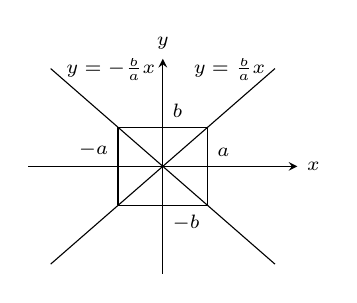
\begin{tikzpicture}[font=\scriptsize,declare function={f(\x)=sqrt(5)/2*sqrt(\x^2-4);fda(\x)=sqrt(5)/2*\x;fdb(\x)=-sqrt(5)/2*\x;}]
\pgfmathsetmacro{\b}{sqrt(5)}
\pgfmathsetmacro{\a}{2}
\pgfmathsetmacro{\n}{\b/2*sqrt(3.5*3.5-4)}
\begin{axis}[width=5cm,axis lines=middle,xlabel={$x$},ylabel={$y$},xlabel style={at={(current axis.right of origin)},anchor=west},ylabel style={at={(current axis.above origin)},anchor=south},xtick={\empty},ytick={\empty},enlargelimits=true, xmin=-5, xmax=5, ymin=-5.123,ymax=5.123]
\addplot[]plot coordinates {(-\a,-\b)(-\a,\b)(\a,\b)(\a,-\b)(-\a,-\b)};
\addplot[]plot coordinates{(-\a,0)}node[above left]{$-a$};
\addplot[]plot coordinates{(\a,0)}node[above right]{$a$};
\addplot[]plot coordinates{(0,\b)}node[above right]{$b$}  {(0,-\b)}node[below right]{$-b$};
\addplot[domain=-5:5]{fda(x)}node[left]{$y=\frac{b}{a}x$};
\addplot[domain=-5:5]{fdb(x)}node[pos=0,right,xshift=0.5ex]{$y=-\frac{b}{a}x$};
\end{axis}
\end{tikzpicture}
\caption{}
\end{subfigure}\hfill
\begin{subfigure}{0.3\textwidth}
\centering
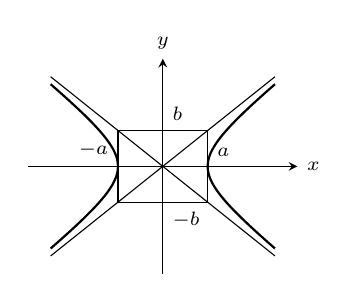
\begin{tikzpicture}[font=\scriptsize,declare function={f(\x)=sqrt(5)/2*sqrt(\x^2-4);fda(\x)=sqrt(5)/2*\x;fdb(\x)=-sqrt(5)/2*\x;}]
\pgfmathsetmacro{\a}{2}
\pgfmathsetmacro{\c}{3}
\pgfmathsetmacro{\b}{sqrt(\c^2-\a^2)}
\pgfmathsetmacro{\n}{\b/2*sqrt(3.5*3.5-4)}
\begin{axis}[width=5cm,axis lines=middle,xlabel={$x$},ylabel={$y$},xlabel style={at={(current axis.right of origin)},anchor=west},ylabel style={at={(current axis.above origin)},anchor=south},xtick={\empty},ytick={\empty},enlargelimits=true]
\addplot[]plot coordinates {(-\a,-\b)(-\a,\b)(\a,\b)(\a,-\b)(-\a,-\b)};
\addplot[]plot coordinates{(-\a,0)}node[above left]{$-a$};
\addplot[]plot coordinates{(\a,0)}node[above right]{$a$};
\addplot[]plot coordinates{(0,\b)}node[above right]{$b$}  {(0,-\b)}node[below right]{$-b$};
\addplot[domain=-5:5]{fda(x)};
\addplot[domain=-5:5]{fdb(x)};
\addplot[thick,domain=2:2.25]{f(x)};
\addplot[thick,domain=2.25:5]{f(x)};
\addplot[thick,domain=2:2.25]{-f(x)};
\addplot[thick,domain=2.25:5]{-f(x)};
\addplot[thick,domain=2:2.25](-x,{f(x)});
\addplot[thick,domain=2.25:5](-x,{f(x)});
\addplot[thick,domain=2:2.25](-x,{-f(x)});
\addplot[thick,domain=2.25:5](-x,{-f(x)});
\end{axis}
\end{tikzpicture}
\caption{}
\end{subfigure}
\caption{متقارب کی مدد سے قطع زائد کی ترسیم۔}
\label{شکل_مخروط_متقارب_سے_قطع_زائد}
\end{figure}

\ابتدا{مثال}\شناخت{مثال_مخروط_ماسکہ_افقی_محور_پر}\ترچھا{محور \عددی{x} پر ماسکے}\\
درج ذیل قطع زائد کی مساوات ہے (شکل \حوالہ{شکل_مثال_مخروط_ماسکہ_افقی_محور_پر})
\begin{align*}
\frac{x^2}{4}-\frac{y^2}{5}=1
\end{align*}
جس میں \عددی{a^2=4} اور \عددی{b^2=5} ہیں (مساوات \حوالہ{مساوات_مخروط_قطع_زائد})۔ یوں درج ذیل ہوں گے۔
\begin{align*}
c&=\sqrt{a^2+b^2}=\sqrt{4+5}=3&&\text{\RL{مرکز سے ماسکہ تک فاصلہ}}\\
(\pm c,0)&=(\pm 3,0)&&\text{ماسکے}\\
(\pm a,0)&=(\pm 2,0)&&\text{راس}\\
y&=\pm \frac{\sqrt{5}}{2}x&&\text{متقارب}
\end{align*}
\انتہا{مثال}
%================
\begin{figure}
\centering
\begin{minipage}{0.45\textwidth}
\centering
\begin{tikzpicture}[declare function={f(\x)=sqrt(5)/2*sqrt(\x^2-4);fd(\x)=sqrt(5/4)*\x;}]
\begin{axis}[clip=false,small,axis lines=middle,xlabel={$x$},ylabel={$y$},xlabel style={at={(current axis.right of origin)},anchor=west}, ylabel style={at={(current axis.above origin)},anchor=south},xtick={\empty},ytick={\empty}]
\addplot[domain=2:2.5]{f(x)};
\addplot[domain=2.5:8]{f(x)};
\addplot[domain=2:2.5]{-f(x)};
\addplot[domain=2.5:8]{-f(x)};
\addplot[domain=2:2.5](-x,{f(x)});
\addplot[domain=2.5:8](-x,{f(x)});
\addplot[domain=2:2.5](-x,{-f(x)});
\addplot[domain=2.5:8](-x,{-f(x)});
\addplot[domain=-8:8]{fd(x)}node[left,yshift=1ex]{$y=\frac{\sqrt{5}}{2}x$};
\addplot[domain=-8:8]{-fd(x)}node[pos=0,right,yshift=1ex]{$y=-\frac{\sqrt{5}}{2}x$};
\addplot[]plot coordinates {(3,0)}node[circ]{}node[above right]{$F(3,0)$}   {(-3,0)}node[circ]{}node[above left]{$F(-3,0)$};
\addplot[]plot coordinates {(2,0)}node[circ]{}node[pin=-40:{$2$}]{}  {(-2,0)}node[circ]{}node[pin=-140:{$-2$}]{};
\addplot[]plot coordinates {(4,4)}node[right,font=\scriptsize]{$\frac{x^2}{4}-\frac{y^2}{5}=1$};
\end{axis}
\end{tikzpicture}
\caption{قطع زائد (مثال \حوالہ{مثال_مخروط_ماسکہ_افقی_محور_پر})}
\label{شکل_مثال_مخروط_ماسکہ_افقی_محور_پر}
\end{minipage}\hfill
\begin{minipage}{0.45\textwidth}
\centering
\begin{tikzpicture}[declare function={f(\x)=2/sqrt(5)*sqrt(\x^2+5);fd(\x)=sqrt(4/5)*\x;}]
\begin{axis}[clip=false,small,axis lines=middle,xlabel={$x$},ylabel={$y$},xlabel style={at={(current axis.right of origin)},anchor=west}, ylabel style={at={(current axis.above origin)},anchor=south},xtick={\empty},ytick={\empty}]
\addplot[domain=-6:6]{f(x)};
\addplot[domain=-6:6]{-f(x)};
\addplot[domain=-6:6]{fd(x)}node[pos=0.75,right,yshift=-0.5ex]{$y=\frac{2}{\sqrt{5}}x$};
\addplot[domain=-6:6]{-fd(x)}node[pos=0.25,left,yshift=-0.5ex]{$y=-\frac{2}{\sqrt{5}}x$};
\addplot[]plot coordinates {(0,3)}node[circ]{}node[above right]{$F(0,3)$}   {(0,-3)}node[circ]{}node[below right]{$F(0,-3)$};
\addplot[]plot coordinates {(0,2)}node[circ]{}node[below left]{$2$}  {(0,-2)}node[circ]{}node[above left]{$-2$};
\addplot[]plot coordinates {(1,5)}node[above right]{$\frac{y^2}{4}-\frac{x^2}{5}=1$};
\end{axis}
\end{tikzpicture}
\caption{قطع زائد (مثال \حوالہ{مثال_مخروط_ماسکہ_عمودی_محور_پر})}
\label{شکل_مثال_مخروط_ماسکہ_عمودی_محور_پر}
\end{minipage}
\end{figure}

\ابتدا{مثال}\شناخت{مثال_مخروط_ماسکہ_عمودی_محور_پر}
درج ذیل قطع زائد کو  مثال \حوالہ{مثال_مخروط_ماسکہ_افقی_محور_پر} کے قطع زائد میں \عددی{x} اور \عددی{y} کو ایک دوسرے کے ساتھ بدل کر حاصل کیا گیا ہے۔ 
\begin{align*}
\frac{y^2}{4}-\frac{x^2}{5}=1
\end{align*}
اس قطع زائد کے راس عمودی محور پر پائے جائیں گے (شکل \حوالہ{شکل_مثال_مخروط_ماسکہ_عمودی_محور_پر})۔ اب بھی \عددی{a^2=4} اور \عددی{b^2=5} ہوں گے۔یوں درج ذیل ہو گا۔
\begin{align*}
c&=\sqrt{a^2+b^2}=\sqrt{4+5}=3&&\text{\RL{مرکز سے ماسکہ تک فاصلہ}}\\
(0,\pm c)&=(0,\pm 3)&&\text{ماسکے}\\
(0,\pm a)&=(0,\pm 2)&&\text{راس}\\
&(0,0)&&\text{مرکز}\\
y&=\pm \frac{2}{\sqrt{5}}x&&\text{متقارب}
\end{align*}
\انتہا{مثال}
%==================

\جزوحصہء{عکسی خواص}
قطع مکافی کا اہم ترین استعمال بطور  شعاع اور ریڈیو امواج کا عاکس ہے۔ قطع مکافی کے ماسکہ سے خارج شعاع، قطع مکافی کے محور کے متوازی منعکس ہوتا ہے (شکل \حوالہ{شکل_مخروط_قطع_مکافی_آئینہ_خاصیت})۔ یہ خاصیت ہاتھ بتی اور گاڑیوں کی اگلی بتیوں میں بروئے کار لایا جاتا ہے۔ اس کے علاوہ خرد امواج نشر کرنے کے لئے بھی قطع مکافی اینٹینا استعمال کیا جاتا ہے جو نقطہ منبع سے خارج برقناطیسی امواج کو ایک محدود شعاع  کی صورت میں خارج کرتا ہے۔ اس کے برعکس قطع مکافی عاکس کے محور کے متوازی آمد  برقناطیسی امواج عاکس کے ماسکہ پر مرکوز کیے جاتے ہیں (شکل \حوالہ{شکل_مخروط_دور_بینی_آئینہ})۔اس خاصیت کی بنا ٹیلی وژن کا ڈش اینٹینا یا ریڈیو دوربین  کمزور اشارات کو اکٹھے کر کے زیادہ طاقتور اشارہ حاصل کرتا ہے۔
اسی طرح سورج کی روشنی کو ایک نقطہ پر مرتکز کیا جا سکتا ہے۔

\begin{figure}
\centering
\begin{minipage}{0.3\textwidth}
\centering
\begin{tikzpicture}[declare function={f(\x)=2*(\x)^2;}]
\pgfmathsetmacro{\a}{0.15}
\pgfmathsetmacro{\b}{0.3}
\pgfmathsetmacro{\c}{0.45}
\begin{axis}[axis equal,width=5cm, axis line style={draw=none},tick style={draw=none},xtick={\empty},ytick={\empty}]
\addplot[thick,domain=0:0.62]({f(x)},x);
\addplot[thick,domain=0:0.62]({f(x)},-x);
\addplot[]plot coordinates{(0.5,0)}node[circ]{};
\addplot[->-=0.75]plot coordinates  {(0.5,0)({f(\a)},\a)};
\addplot[->-=0.75]plot coordinates  {({f(\a)},\a)(1.5,\a)};
\addplot[->-=0.75]plot coordinates  {(0.5,0)({f(\b)},\b)};
\addplot[->-=0.75]plot coordinates  {({f(\b)},\b)(1.5,\b)};
\addplot[->-=0.75]plot coordinates  {(0.5,0)({f(\c)},\c)};
\addplot[->-=0.75]plot coordinates  {({f(\c)},\c)(1.5,\c)};
\addplot[->-=0.75]plot coordinates  {(0.5,0)({f(\a)},-\a)};
\addplot[->-=0.75]plot coordinates  {({f(\a)},-\a)(1.5,-\a)};
\addplot[->-=0.75]plot coordinates  {(0.5,0)({f(\b)},-\b)};
\addplot[->-=0.75]plot coordinates  {({f(\b)},-\b)(1.5,-\b)};
\addplot[->-=0.75]plot coordinates  {(0.5,0)({f(\c)},-\c)};
\addplot[->-=0.75]plot coordinates  {({f(\c)},-\c)(1.5,-\c)};
\end{axis}
\end{tikzpicture}
\caption{قطع مکافی آئینہ کے ماسکہ سے نکلتا شعاع انعکاس کے بعد محور کے متوازی ہو گا۔}
\label{شکل_مخروط_قطع_مکافی_آئینہ_خاصیت}
\end{minipage}\hfill
\begin{minipage}{0.3\textwidth}
\centering
\begin{tikzpicture}[declare function={f(\x)=2*(\x)^2;}]
\pgfmathsetmacro{\a}{0.15}
\pgfmathsetmacro{\b}{0.3}
\pgfmathsetmacro{\c}{0.45}
\begin{scope}[rotate=30]
\begin{axis}[axis equal,width=5cm, axis line style={draw=none},tick style={draw=none},xtick={\empty},ytick={\empty}]
\addplot[thick,domain=0:0.62]({f(x)},x);
\addplot[thick,domain=0:0.62]({f(x)},-x);
\addplot[]plot coordinates{(0.5,0)}node[circ]{};
\addplot[-<-=0.75]plot coordinates  {(0.5,0)({f(\a)},\a)};
\addplot[-<-=0.75]plot coordinates  {({f(\a)},\a)(1.5,\a)};
\addplot[-<-=0.75]plot coordinates  {(0.5,0)({f(\b)},\b)};
\addplot[-<-=0.75]plot coordinates  {({f(\b)},\b)(1.5,\b)};
\addplot[-<-=0.75]plot coordinates  {(0.5,0)({f(\c)},\c)};
\addplot[-<-=0.75]plot coordinates  {({f(\c)},\c)(1.5,\c)};
\addplot[-<-=0.75]plot coordinates  {(0.5,0)({f(\a)},-\a)};
\addplot[-<-=0.75]plot coordinates  {({f(\a)},-\a)(1.5,-\a)};
\addplot[-<-=0.75]plot coordinates  {(0.5,0)({f(\b)},-\b)};
\addplot[-<-=0.75]plot coordinates  {({f(\b)},-\b)(1.5,-\b)};
\addplot[-<-=0.75]plot coordinates  {(0.5,0)({f(\c)},-\c)};
\addplot[-<-=0.75]plot coordinates  {({f(\c)},-\c)(1.5,-\c)};
\end{axis}
\end{scope}
\end{tikzpicture}
\caption{قطع مکافی عاکس پر آمد شعاع ماسکہ پر پہنچتا ہے۔}
\label{شکل_مخروط_دور_بینی_آئینہ}
\end{minipage}\hfill
\begin{minipage}{0.3\textwidth}
\centering
\begin{tikzpicture}[declare function={f(\x)=1.5/2*sqrt(2^2-(\x)^2);}]
\pgfmathsetmacro{\c}{sqrt(2^2-1.5^2)}
\begin{axis}[axis equal,width=5cm,axis line style={draw=none},tick style={draw=none},xtick={\empty},ytick=\empty]
\addplot[thick,domain=-2:-2+0.2]{f(x)};
\addplot[thick,domain=-2+0.2:2-0.2]{f(x)};
\addplot[thick,domain=2-0.2:2]{f(x)};
\addplot[thick,domain=-2:-2+0.2]{-f(x)};
\addplot[thick,domain=-2+0.2:2-0.2]{-f(x)};
\addplot[thick,domain=2-0.2:2]{-f(x)};
\addplot[]plot coordinates{(-\c,0)}node[circ]{}node[below]{$F_1$};
\addplot[]plot coordinates{(\c,0)}node[circ]{}node[below]{$F_2$};
\addplot[->-=0.5]plot coordinates {(-\c,0)(1.3,{f(1.3)})};
\addplot[->-=0.5]plot coordinates {(1.3,{f(1.3)})(\c,0)};
\end{axis}
\end{tikzpicture}
\caption{ترخیم کے ایک ماسکہ سے خارج شعاع دوسرے ماسکہ پر پہنچتا ہے۔}
\label{شکل_مخروط_ترخیم_کمرہ_سرگوشی}
\end{minipage}
\end{figure}

ایک ترخیم کو اس کے محور کے گرد گھما کر سطح طواف پیدا کیا جا سکتا ہے جو \اصطلاح{ترخیمی سطح}\فرہنگ{ترخیمی سطح}\حاشیہب{ellipsoid}\فرہنگ{ellipsoid} کہلاتا ہے۔اس کی اندرونی سطح پر چاندی کی تہہ لگا کر آئینہ بنایا جا سکتا ہے۔ ایک ماسکہ سے خارج شعاع دوسرے ماسکہ پر منعکس ہو گا (شکل \حوالہ{شکل_مخروط_ترخیم_کمرہ_سرگوشی} اور سوال \حوالہ{سوال_مخروط_کمرہ_سرگوشی})۔ ترخیمی سطح اسی طرح آواز کو بھی ایک ماسکہ سے دوسرے ماسکہ منتقل کرتا ہے۔ اس خاصیت کو استعمال کرتے ہوئے کمرہ سرگوشی بنایا جا سکتا ہے جس میں ایک ماسکہ پر بیٹھا شخص دوسرے ماسکہ پر بیٹھے شخص کے ساتھ سرگوشی سے باتیں کر سکتا ہے۔ کمرہ سرگوشی میں موجود باقی لوگ ان کی باتیں سننے  سے قاصر ہوں  گے۔ ہوائی جہازوں کی کارکردگی پر ہوائی سرنگ میں غور کیا جاتا ہے۔ جہاز کے شور پر غور کرتے ہوئے نقطہ غور کو ترخیمی سطح کے ایک ماسکہ پر رکھا جاتا ہے جبکہ مائکروفون  کو  اس کی دوسرے ماسکہ پر رکھا جاتا ہے۔ دیگر نقطوں سے پیدا شور کے اثر کو یوں بہت کم کرنا ممکن ہوتا ہے۔

قطع زائد آئینہ کے ایک ماسکہ پر آمد شعاع کو آئینہ دوسرے ماسکہ پر بھیجتا ہے۔ قطع مکافی سطح، ترخیمی سطح اور قطع مکافی سطحوں کے خواص کو استعمال کرتے ہوئے جدید دور بین تیار کیے جاتے ہیں۔   

\جزوحصہء{سوالات}
\موٹا{ترسیم کی پہچان}\\
سوال \حوالہ{سوال_مخروط_ہم_پلہ_الف} تا سوال \حوالہ{سوال_مخروط_ہم_پلہ_ب} میں دی  گئی قطع مکافی کی مساوات درج ذیل میں تلاش کریں۔
\begin{align*}
x^2=2y,\quad x^2=-6y,\quad y^2=8x,\quad y^2=-4x
\end{align*}
اس کے بعد قطع مکافی کے ماسکہ اور ناظمہ دریافت کریں۔

%=============================
\ابتدا{سوال}\شناخت{سوال_مخروط_ہم_پلہ_الف}
شکل \حوالہ{شکل_مخروط_ترخیم_بائیں_دائیں}-ا\\
جواب:\quad
\عددی{y^2=8x}، ماسکہ \عددی{F(2,0)} اور ناظمہ \عددی{x=-2}
\انتہا{سوال}
%===================
\ابتدا{سوال}
شکل \حوالہ{شکل_مخروط_ترخیم_بائیں_دائیں}-ب
\انتہا{سوال}
%===================
\ابتدا{سوال}
شکل \حوالہ{شکل_مخروط_ترخیم_بائیں_دائیں}-ج\\
جواب:\quad
\عددی{x^2=-6y}، ماسکہ \عددی{F(0,-\tfrac{3}{2})} اور ناظمہ \عددی{y=\tfrac{3}{2}}
\انتہا{سوال}
%===================
\ابتدا{سوال}\شناخت{سوال_مخروط_ہم_پلہ_ب}
شکل \حوالہ{شکل_مخروط_ترخیم_بائیں_دائیں}-د
\انتہا{سوال}
%===================
\begin{figure}
\centering
\begin{subfigure}{0.22\textwidth}
\centering
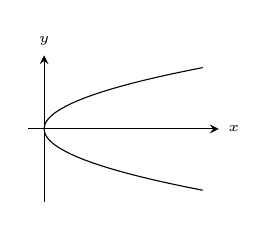
\begin{tikzpicture}[font=\tiny,declare function={f(\x)=2*sqrt(\x);}]
\begin{axis}[width=4cm,axis lines=middle,xlabel={$x$},ylabel={$y$},xlabel style={at={(current axis.right of origin)},anchor=west},ylabel style={at={(current axis.above origin)},anchor=south},xtick={\empty},ytick={\empty},enlargelimits]
\addplot[domain=0:0.2]{f(x)};
\addplot[domain=0.2:2]{f(x)};
\addplot[domain=0:0.2]{-f(x)};
\addplot[domain=0.2:2]{-f(x)};
\end{axis}
\end{tikzpicture}
\caption{}
\end{subfigure}\hfill
\begin{subfigure}{0.22\textwidth}
\centering
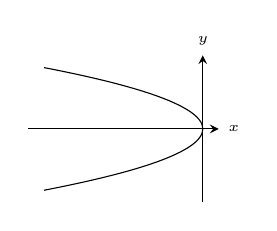
\begin{tikzpicture}[font=\tiny,declare function={f(\x)=2*sqrt(-\x);}]
\begin{axis}[width=4cm,axis lines=middle,xlabel={$x$},ylabel={$y$},xlabel style={at={(current axis.right of origin)},anchor=west},ylabel style={at={(current axis.above origin)},anchor=south},xtick={\empty},ytick={\empty},enlargelimits=true]
\addplot[domain=0:-0.2]{f(x)};
\addplot[domain=-0.2:-2]{f(x)};
\addplot[domain=0:-0.2]{-f(x)};
\addplot[domain=-0.2:-2]{-f(x)};
\end{axis}
\end{tikzpicture}
\caption{}
\end{subfigure}\hfill
\begin{subfigure}{0.22\textwidth}
\centering
\begin{tikzpicture}[font=\tiny,declare function={f(\x)=-1/4*\x^2;}]
\begin{axis}[width=4cm,axis lines=middle,xlabel={$x$},ylabel={$y$},xlabel style={at={(current axis.right of origin)},anchor=west},ylabel style={at={(current axis.above origin)},anchor=south},xtick={\empty},ytick={\empty},enlargelimits]
\addplot[domain=0:0.2]{f(x)};
\addplot[domain=0.2:2]{f(x)};
\addplot[domain=0:0.2](-x,{f(x)});
\addplot[domain=0.2:2](-x,{f(x)});
\end{axis}
\end{tikzpicture}
\caption{}
\end{subfigure}\hfill
\begin{subfigure}{0.22\textwidth}
\centering
\begin{tikzpicture}[font=\tiny,declare function={f(\x)=1/4*\x^2;}]
\begin{axis}[width=4cm,axis lines=middle,xlabel={$x$},ylabel={$y$},xlabel style={at={(current axis.right of origin)},anchor=west},ylabel style={at={(current axis.above origin)},anchor=south},xtick={\empty},ytick={\empty},enlargelimits=true]
\addplot[domain=0:0.2]{f(x)};
\addplot[domain=0.2:2]{f(x)};
\addplot[domain=0:0.2](-x,{f(x)});
\addplot[domain=0.2:2](-x,{f(x)});
\end{axis}
\end{tikzpicture}
\caption{}
\end{subfigure}
\caption{ترسیم برائے سوال \حوالہ{سوال_مخروط_ہم_پلہ_الف} تا سوال \حوالہ{سوال_مخروط_ہم_پلہ_ب}}
\label{شکل_مخروط_ترخیم_بائیں_دائیں}
\end{figure}

سوال \حوالہ{سوال_مخروط_ہم_پلہ_تلاش_الف} تا سوال \حوالہ{سوال_مخروط_ہم_پلہ_تلاش_ب} میں دیے گئے مخروط کی مساوات درج ذیل میں تلاش کریں۔
\begin{align*}
\frac{x^2}{4}+\frac{y^2}{9}=1,\quad \frac{x^2}{2}+y^2=1,\quad \frac{y^2}{4}-x^2=1,\quad \frac{x^2}{4}-\frac{y^2}{9}=1
\end{align*}
دیے گئے مخروط کا ماسکہ اور راس تلاش کریں۔ اگر قطع زائد دیا گیا ہو تب اس کے متقارب بھی دریافت کریں۔

\ابتدا{سوال}\شناخت{سوال_مخروط_ہم_پلہ_تلاش_الف}
ترسیم شکل \حوالہ{شکل_مخروط_کئی_الف}-ا میں دیا گیا ہے۔\\
جواب:\quad
\عددی{\tfrac{x^2}{4}-\tfrac{y^2}{9}=1}، ماسکے \عددی{F(\pm\sqrt{13},0)}، راس \عددی{V(\pm 2,0)} اور متقارب \عددی{y=\pm\tfrac{3}{2}x}
\انتہا{سوال}
%===================
\ابتدا{سوال}
ترسیم شکل \حوالہ{شکل_مخروط_کئی_الف}-ب میں دیا گیا ہے۔
\انتہا{سوال}
%========================
\ابتدا{سوال}
ترسیم شکل \حوالہ{شکل_مخروط_کئی_الف}-ج میں دیا گیا ہے۔\\
جواب:\quad
\عددی{\tfrac{x^2}{2}+y^2=1}، ماسکے \عددی{F(\pm 1,0)}، راس \عددی{V(\pm\sqrt{2},0)}
\انتہا{سوال}
%========================
\ابتدا{سوال}\شناخت{سوال_مخروط_ہم_پلہ_تلاش_ب}
ترسیم شکل \حوالہ{شکل_مخروط_کئی_الف}-د میں دیا گیا ہے۔
\انتہا{سوال}
%========================
\begin{figure}
\centering
\begin{subfigure}{0.22\textwidth}
\centering
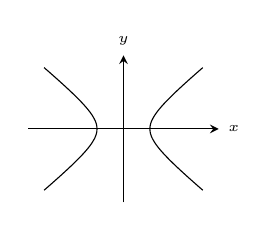
\begin{tikzpicture}[font=\tiny,declare function={f(\x)=sqrt(5)/2*sqrt(\x^2-4);}]
\begin{axis}[width=4cm,axis lines=middle,xlabel={$x$},ylabel={$y$},xlabel style={at={(current axis.right of origin)},anchor=west},ylabel style={at={(current axis.above origin)},anchor=south},xtick={\empty},ytick={\empty},enlargelimits]
\addplot[domain=2:2.2]{f(x)};
\addplot[domain=2.2:6]{f(x)};
\addplot[domain=2:2.2]{-f(x)};
\addplot[domain=2.2:6]{-f(x)};
\addplot[domain=2:2.2](-x,{f(x)});
\addplot[domain=2.2:6](-x,{f(x)});
\addplot[domain=2:2.2](-x,{-f(x)});
\addplot[domain=2.2:6](-x,{-f(x)});
\end{axis}
\end{tikzpicture}
\caption{}
\end{subfigure}\hfill
\begin{subfigure}{0.22\textwidth}
\centering
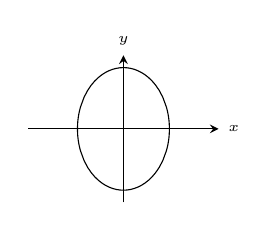
\begin{tikzpicture}[font=\tiny,declare function={f(\x)=4/3*sqrt(9-\x^2);}]
\begin{axis}[width=4cm,axis equal,axis lines=middle,xlabel={$x$},ylabel={$y$},xlabel style={at={(current axis.right of origin)},anchor=west},ylabel style={at={(current axis.above origin)},anchor=south},xtick={\empty},ytick={\empty},enlargelimits]
\addplot[domain=-3:-2.8]{f(x)};
\addplot[domain=-2.8:2.8]{f(x)};
\addplot[domain=2.8:3]{f(x)};
\addplot[domain=-3:-2.8]{-f(x)};
\addplot[domain=-2.8:2.8]{-f(x)};
\addplot[domain=2.8:3]{-f(x)};
\end{axis}
\end{tikzpicture}
\caption{}
\end{subfigure}\hfill
\begin{subfigure}{0.22\textwidth}
\centering
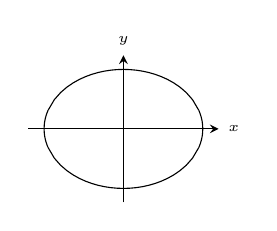
\begin{tikzpicture}[font=\tiny,declare function={f(\x)=3/4*sqrt(16-\x^2);}]
\begin{axis}[width=4cm,axis equal,axis lines=middle,xlabel={$x$},ylabel={$y$},xlabel style={at={(current axis.right of origin)},anchor=west},ylabel style={at={(current axis.above origin)},anchor=south},xtick={\empty},ytick={\empty},enlargelimits]
\addplot[domain=-4:-3.8]{f(x)};
\addplot[domain=-3.8:3.8]{f(x)};
\addplot[domain=3.8:4]{f(x)};
\addplot[domain=-4:-3.8]{-f(x)};
\addplot[domain=-3.8:3.8]{-f(x)};
\addplot[domain=3.8:4]{-f(x)};
\end{axis}
\end{tikzpicture}
\caption{}
\end{subfigure}\hfill
\begin{subfigure}{0.22\textwidth}
\centering
\begin{tikzpicture}[font=\tiny,declare function={f(\x)=2/sqrt(5)*sqrt(5+\x^2);}]
\begin{axis}[width=4cm,axis equal,axis lines=middle,xlabel={$x$},ylabel={$y$},xlabel style={at={(current axis.right of origin)},anchor=west},ylabel style={at={(current axis.above origin)},anchor=south},xtick={\empty},ytick={\empty},enlargelimits]
\addplot[domain=-4:4]{f(x)};
\addplot[domain=-4:4]{-f(x)};
\end{axis}
\end{tikzpicture}
\caption{}
\end{subfigure}
\caption{ترسیمات برائے سوال \حوالہ{سوال_مخروط_ہم_پلہ_تلاش_الف} تا سوال \حوالہ{سوال_مخروط_ہم_پلہ_تلاش_ب}}
\label{شکل_مخروط_کئی_الف}
\end{figure}

\موٹا{قطع مکافی}\\
سوال \حوالہ{سوال_مخروط_قطع_مکافی_دیا_الف} تا سوال \حوالہ{سوال_مخروط_قطع_مکافی_دیا_ٹ} میں دیے گئے قطع مکافی کا ماسکہ اور ناظمہ تلاش کرنے کے بعد  اس کو ترسیم کریں۔ ماسکہ اور ناظمہ کو بھی ترسیم میں شامل کریں۔

\ابتدا{سوال}\شناخت{سوال_مخروط_قطع_مکافی_دیا_الف}
$y^2=12x$\\
جواب:\quad
شکل \حوالہ{شکل_سوال_مخروط_قطع_مکافی_دیا_الف}
\انتہا{سوال}
%=====================
\ابتدا{سوال}
$x^2=6y$
\انتہا{سوال}
%=====================
\ابتدا{سوال}\شناخت{سوال_مخروط_قطع_مکافی_دیا_ب}
$x^2=-8y$\\
جواب:\quad
شکل \حوالہ{شکل_سوال_مخروط_قطع_مکافی_دیا_ب}
\انتہا{سوال}
%=====================
\ابتدا{سوال}
$y^2=-2x$
\انتہا{سوال}
%=====================
\ابتدا{سوال}\شناخت{سوال_مخروط_قطع_مکافی_دیا_پ}
$y=4x^2$\\
جواب:\quad
شکل \حوالہ{شکل_سوال_مخروط_قطع_مکافی_دیا_پ}
\انتہا{سوال}
%=====================
\ابتدا{سوال}
$y=-8x^2$
\انتہا{سوال}
%=====================
\ابتدا{سوال}\شناخت{سوال_مخروط_قطع_مکافی_دیا_ت}
$x=-3y^2$\\
جواب:\quad
شکل \حوالہ{شکل_سوال_مخروط_قطع_مکافی_دیا_ت}
\انتہا{سوال}
%=====================
\ابتدا{سوال}\شناخت{سوال_مخروط_قطع_مکافی_دیا_ٹ}
$x=2y^2$
\انتہا{سوال}
%=====================
\begin{figure}
\centering
\begin{minipage}{0.22\textwidth}
\begin{tikzpicture}[font=\tiny,declare function={f(\x)=sqrt(12*\x);}]
\begin{axis}[clip=false,width=4cm,axis lines=middle,xlabel={$x$},ylabel={$y$},xlabel style={at={(current axis.right of origin)},anchor=west},ylabel style={at={(current axis.above origin)},anchor=south},enlargelimits=true,xtick={-3},ytick={3}]
\addplot[domain=0:0.2]{f(x)};
\addplot[domain=0.2:4]{f(x)}node[pos=0.75,below right]{$y^2=12x$};
\addplot[domain=0:0.2]{-f(x)};
\addplot[domain=0.2:4]{-f(x)};
\addplot[]plot coordinates {(-3,-7)(-3,7)}node[pos=0.85,right]{$x=-3$};
\addplot[]plot coordinates {(3,0)}node[circ]{}node[below]{$F(3,0)$};
\end{axis}
\end{tikzpicture}
\caption{}
\label{شکل_سوال_مخروط_قطع_مکافی_دیا_الف}
\end{minipage}\hfill
\begin{minipage}{0.22\textwidth}
\begin{tikzpicture}[font=\tiny,declare function={f(\x)=-1/8*(\x)^2;}]
\begin{axis}[width=4cm,axis lines=middle,xlabel={$x$},ylabel={$y$},xlabel style={at={(current axis.right of origin)},anchor=west},ylabel style={at={(current axis.above origin)},anchor=south},enlargelimits=true,xtick={2},ytick={2},y tick label style={yshift=0.5ex}]
\addplot[domain=-3:3]{f(x)}node[pos=0.25,below,yshift=-0.5ex]{$x^2=-8y$};
\addplot[]plot coordinates {(-3,2)(3,2)}node[pos=0.85,below]{$y=2$};
\addplot[]plot coordinates {(0,-2)}node[circ]{}node[right]{$F(0,-2)$};
\end{axis}
\end{tikzpicture}
\caption{}
\label{شکل_سوال_مخروط_قطع_مکافی_دیا_ب}
\end{minipage}\hfill
\begin{minipage}{0.22\textwidth}
\begin{tikzpicture}[font=\tiny,declare function={f(\x)=4*(\x)^2;}]
\pgfmathsetmacro{\d}{1/16}
\begin{axis}[clip=false,width=4cm,axis lines=middle,xlabel={$x$},ylabel={$y$},xlabel style={at={(current axis.right of origin)},anchor=west},ylabel style={at={(current axis.above origin)},anchor=south},enlargelimits=true,xtick={0.25},ytick={0.25},xticklabels={$\tfrac{1}{4}$},yticklabels={$\tfrac{1}{4}$}]
\addplot[domain=-0.3:0.3]{f(x)}node[left]{$y=4x^2$};
\addplot[]plot coordinates {(-0.3,-\d)(0.3,-\d)}node[pos=0.15,below]{$y=-\tfrac{1}{16}$};
\addplot[]plot coordinates {(0,\d)}node[circ]{}node[right]{$F(0,\tfrac{1}{16})$};
\end{axis}
\end{tikzpicture}
\caption{}
\label{شکل_سوال_مخروط_قطع_مکافی_دیا_پ}
\end{minipage}\hfill
\begin{minipage}{0.22\textwidth}
\begin{tikzpicture}[font=\tiny,declare function={f(\x)=sqrt(-1/3*\x);}]
\pgfmathsetmacro{\d}{1/12}
\pgfmathsetmacro{\yt}{1/6}
\begin{axis}[clip=false,width=4cm,axis lines=middle,xlabel={$x$},ylabel={$y$},xlabel style={at={(current axis.right of origin)},anchor=west},ylabel style={at={(current axis.above origin)},anchor=south},enlargelimits=true,xtick={\d},ytick={-\yt,\yt},xticklabels={\hspace*{2ex}$\tfrac{1}{12}$},yticklabels={$-\tfrac{1}{6}$,$\tfrac{1}{6}$}]
\addplot[domain=-0.15:0]{f(x)}node[pos=0,below]{$x=-3y^2$};
\addplot[domain=-0.15:0]{-f(x)};
\addplot[]plot coordinates {(\d,-0.2)(\d,0.2)}node[above]{$x=\tfrac{1}{12}$};
\addplot[]plot coordinates {(-\d,0)}node[circ]{}node[below]{$F(-\tfrac{1}{12},0)$};
\end{axis}
\end{tikzpicture}
\caption{}
\label{شکل_سوال_مخروط_قطع_مکافی_دیا_ت}
\end{minipage}
\end{figure}
\موٹا{ترخیم}\\
سوال \حوالہ{سوال_مخروط_ترخیم_دیا_الف} تا سوال \حوالہ{سوال_مخروط_ترخیم_دیا_ٹ} میں دیے گئے ترخیم کی مساوات کو معیاری روپ میں لکھ کر ترسیم کریں۔ ترسیم پر ماسکے  دکھائیں۔ 

\ابتدا{سوال}\شناخت{سوال_مخروط_ترخیم_دیا_الف}
$16x^2+25y^2=400$\\
جواب:\quad
شکل \حوالہ{شکل_سوال_مخروط_ترخیم_دیا_الف}
\انتہا{سوال}
%===================
\ابتدا{سوال}
$7x^2+16y^2=112$
\انتہا{سوال}
%=====================
\ابتدا{سوال}\شناخت{سوال_مخروط_ترخیم_دیا_ب}
$2x^2+y^2=2$\\
جواب:\quad
شکل \حوالہ{شکل_سوال_مخروط_ترخیم_دیا_ب}
\انتہا{سوال}
%=====================
\ابتدا{سوال}
$2x^2+y^2=4$
\انتہا{سوال}
%=====================
\ابتدا{سوال}\شناخت{سوال_مخروط_ترخیم_دیا_پ}
$3x^2+2y^2=6$\\
جواب:\quad
شکل \حوالہ{شکل_سوال_مخروط_ترخیم_دیا_پ}
\انتہا{سوال}
%=====================
\ابتدا{سوال}
$9x^2+10y^2=90$
\انتہا{سوال}
%=====================
\ابتدا{سوال}\شناخت{سوال_مخروط_ترخیم_دیا_ت}
$6x^2+9y^2=54$\\
جواب:\quad
شکل \حوالہ{شکل_سوال_مخروط_ترخیم_دیا_ت}
\انتہا{سوال}
%=====================
\ابتدا{سوال}\شناخت{سوال_مخروط_ترخیم_دیا_ٹ}
$169x^2+25y^2=4225$
\انتہا{سوال}
%=====================
\begin{figure}
\centering
\begin{minipage}{0.22\textwidth}
\begin{tikzpicture}[font=\tiny,declare function={f(\x)=4/5*sqrt(25-(\x)^2);}]
\begin{axis}[clip=false,width=4cm,axis lines=middle,xlabel={$x$},ylabel={$y$},xlabel style={at={(current axis.right of origin)},anchor=west},ylabel style={at={(current axis.above origin)},anchor=south},enlargelimits=true,xtick={-3,3},ytick={-4,4}]
\addplot[domain=-4.8:4.8]{f(x)}node[pos=0.8,above,xshift=1ex]{$\tfrac{x^2}{25}+\tfrac{y^2}{16}=1$};
\addplot[domain=-4.8:4.8]{-f(x)};
\addplot[domain=-5:-4.8]{f(x)};
\addplot[domain=-5:-4.8]{-f(x)};
\addplot[domain=4.8:5]{f(x)};
\addplot[domain=4.8:5]{-f(x)};
\addplot[]plot coordinates {(-3,0)}node[above]{$F_1$}  {(3,0)}node[above]{$F_2$};
\end{axis}
\end{tikzpicture}
\caption{}
\label{شکل_سوال_مخروط_ترخیم_دیا_الف}
\end{minipage}\hfill
\begin{minipage}{0.22\textwidth}
\begin{tikzpicture}[font=\tiny,declare function={f(\x)=sqrt(2-2*(\x)^2);}]
\pgfmathsetmacro{\k}{sqrt(2)}
\begin{axis}[axis equal,clip=false,width=4cm,axis lines=middle,xlabel={$x$},ylabel={$y$},xlabel style={at={(current axis.right of origin)},anchor=west},ylabel style={at={(current axis.above origin)},anchor=south},enlargelimits=true,xtick={-1,1},ytick={-1,1}]
\addplot[domain=-0.8:0.8]{f(x)}node[pos=0.75,above,xshift=3ex]{$x^2+\tfrac{y^2}{2}=1$};
\addplot[domain=-0.8:0.8]{-f(x)};
\addplot[domain=-1:-0.8]{f(x)};
\addplot[domain=0.8:1]{f(x)};
\addplot[domain=-1:-0.8]{-f(x)};
\addplot[domain=0.8:1]{-f(x)};
\addplot[]plot coordinates {(0,1)}node[right]{$F_1$}  {(0,-1)}node[right]{$F_2$};
\addplot[]plot coordinates {(0,\k)}node[shift={(-2ex,0.25ex)}]{$\sqrt{2}$};
\end{axis}
\end{tikzpicture}
\caption{}
\label{شکل_سوال_مخروط_ترخیم_دیا_ب}
\end{minipage}\hfill
\begin{minipage}{0.22\textwidth}
\begin{tikzpicture}[font=\tiny,declare function={f(\x)=sqrt(3/2)*sqrt(2-(\x)^2);}]
\pgfmathsetmacro{\k}{sqrt(2)}
\pgfmathsetmacro{\kk}{sqrt(3)}
\begin{axis}[axis equal,clip=false,width=4cm,axis lines=middle,xlabel={$x$},ylabel={$y$},xlabel style={at={(current axis.right of origin)},anchor=west},ylabel style={at={(current axis.above origin)},anchor=south},enlargelimits=true,xtick={\empty},ytick={-1,1}]
\addplot[domain=-\k+0.2:\k-0.2]{f(x)}node[pos=0.75,above,xshift=3ex]{$\tfrac{x^2}{2}+\tfrac{y^2}{3}=1$};
\addplot[domain=-\k+0.2:\k-0.2]{-f(x)};
\addplot[domain=-\k:-\k+0.2]{f(x)};
\addplot[domain=\k-0.2:\k]{f(x)};
\addplot[domain=-\k:-\k+0.2]{-f(x)};
\addplot[domain=\k-0.2:\k]{-f(x)};
\addplot[]plot coordinates {(0,1)}node[right]{$F_1$}  {(0,-1)}node[right]{$F_2$};
\addplot[]plot coordinates {(\k,0)}node[shift={(1ex,-1ex)}]{$\sqrt{2}$}  {(0,\kk)}node[shift={(-2ex,0.25ex)}]{$\sqrt{3}$};
\end{axis}
\end{tikzpicture}
\caption{}
\label{شکل_سوال_مخروط_ترخیم_دیا_پ}
\end{minipage}\hfill
\begin{minipage}{0.22\textwidth}
\begin{tikzpicture}[font=\tiny,declare function={f(\x)=sqrt(6/9)*sqrt(9-(\x)^2);}]
\pgfmathsetmacro{\k}{sqrt(9)}
\pgfmathsetmacro{\kk}{sqrt(6)}
\pgfmathsetmacro{\kkk}{sqrt(3)}
\begin{axis}[axis equal,clip=false,width=4cm,axis lines=middle,xlabel={$x$},ylabel={$y$},xlabel style={at={(current axis.right of origin)},anchor=west},ylabel style={at={(current axis.above origin)},anchor=south},enlargelimits=true,xtick={-\kkk,\kkk},xticklabels={$-\sqrt{3}$,$\sqrt{3}$},ytick={\empty}]
\addplot[domain=-\k+0.2:\k-0.2]{f(x)}node[pos=0.75,above,xshift=3ex]{$\tfrac{x^2}{9}+\tfrac{y^2}{6}=1$};
\addplot[domain=-\k+0.2:\k-0.2]{-f(x)};
\addplot[domain=-\k:-\k+0.2]{f(x)};
\addplot[domain=\k-0.2:\k]{f(x)};
\addplot[domain=-\k:-\k+0.2]{-f(x)};
\addplot[domain=\k-0.2:\k]{-f(x)};
\addplot[]plot coordinates {(-\kkk,0)}node[above]{$F_1$}  {(\kkk,0)}node[above]{$F_2$};
\addplot[]plot coordinates {(0,\kk)}node[shift={(-2ex,0.25ex)}]{$\sqrt{6}$};
\end{axis}
\end{tikzpicture}
\caption{}
\label{شکل_سوال_مخروط_ترخیم_دیا_ت}
\end{minipage}
\end{figure}

سوال \حوالہ{سوال_مخروط_ترسیم_معلومات_الف} اور سوال \حوالہ{سوال_مخروط_ترسیم_معلومات_ب} میں \عددی{xy} مستوی میں پائے جانے والے  ترخیم کے ماسکہ اور راس  دیے  گئے ہیں۔ ترخیم کا مرکز  \عددی{xy} مستوی کے مبدا پر ہے۔ ترخیم کی معیاری مساوات تلاش کریں۔

\ابتدا{سوال}\شناخت{سوال_مخروط_ترسیم_معلومات_الف}
ماسکے \عددی{(\pm \sqrt{2},0)} اور راس \عددی{(\pm 2,0)}\\
جواب:\quad
$\tfrac{x^2}{4}+\tfrac{y^2}{2}=1$
\انتہا{سوال}
%=======================
\ابتدا{سوال}\شناخت{سوال_مخروط_ترسیم_معلومات_ب}
ماسکے \عددی{(0,\pm 4)} اور راس \عددی{(0,\pm 5)}
\انتہا{سوال}
%========================

\موٹا{قطع زائد}\\
سوال \حوالہ{سوال_مخروط_قطع_زائد_معلومات_الف} تا سوال \حوالہ{سوال_مخروط_قطع_زائد_معلومات_ٹ} میں قطع زائد کی مساواتیں دی گئی ہیں۔ مساوات کو معیاری روپ میں لکھیں اور قطع زائد کا متقارب دریافت کریں۔ قطع زائد کا خاکہ کھینچ کر متقارب اور ماسکہ بھی دکھائیں۔ 

\ابتدا{سوال}\شناخت{سوال_مخروط_قطع_زائد_معلومات_الف}
$x^2-y^2=1$\\
جواب:\quad
متقارب \عددی{y=\pm x} اور شکل \حوالہ{شکل_سوال_مخروط_قطع_زائد_معلومات_الف}
\انتہا{سوال}
%=========================
\ابتدا{سوال}
$9x^2-16y^2=144$
\انتہا{سوال}
%=================================
\ابتدا{سوال}\شناخت{سوال_مخروط_قطع_زائد_معلومات_ب}
$y^2-x^2=8$\\
جواب:\quad
متقارب \عددی{y=\pm x} اور شکل \حوالہ{شکل_سوال_مخروط_قطع_زائد_معلومات_ب}
\انتہا{سوال}
%=================================
\ابتدا{سوال}
$y^2-x^2=4$
\انتہا{سوال}
%=================================
\ابتدا{سوال}\شناخت{سوال_مخروط_قطع_زائد_معلومات_پ}
$8x^2-2y^2=16$\\
جواب:\quad
متقارب \عددی{y=\pm 2x} اور شکل \حوالہ{شکل_سوال_مخروط_قطع_زائد_معلومات_پ}
\انتہا{سوال}
%=================================
\ابتدا{سوال}
$y^2-3x^2=3$
\انتہا{سوال}
%=================================
\ابتدا{سوال}\شناخت{سوال_مخروط_قطع_زائد_معلومات_ت}
$8y^2-2x^2=16$\\
جواب:\quad
متقارب \عددی{y=\pm \tfrac{x}{2}} اور شکل \حوالہ{شکل_سوال_مخروط_قطع_زائد_معلومات_ت}
\انتہا{سوال}
%=================================
\ابتدا{سوال}\شناخت{سوال_مخروط_قطع_زائد_معلومات_ٹ}
$64x^2-36y^2=2304$
\انتہا{سوال}
%=================================
%=====================
\begin{figure}
\centering
\begin{minipage}{0.22\textwidth}
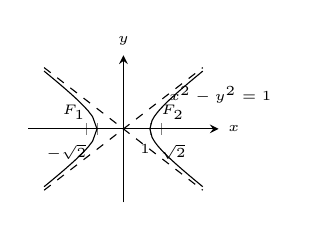
\begin{tikzpicture}[font=\tiny,declare function={f(\x)=sqrt((\x)^2-1);fa(\x)=\x;}]
\pgfmathsetmacro{\f}{sqrt(2)}
\begin{axis}[clip=false,width=4cm,axis lines=middle,xlabel={$x$},ylabel={$y$},xlabel style={at={(current axis.right of origin)},anchor=west},ylabel style={at={(current axis.above origin)},anchor=south},enlargelimits=true,xtick={-\f,\f,1,-1},xticklabels={\llap{$-\sqrt{2}$},\rlap{$\sqrt{2}$},\llap{$1$},},ytick={\empty}]
\addplot[domain=-3:1]{f(x)};
\addplot[domain=-3:1]{-f(x)};
\addplot[domain=1:3]{f(x)}node[pos=0.9,below,xshift=2ex]{$x^2-y^2=1$};
\addplot[domain=1:3]{-f(x)};
\addplot[dashed,domain=-3:3]{fa(x)};
\addplot[dashed,domain=-3:3]{-fa(x)};
\addplot[]plot coordinates {(-\f,0)}node[above,xshift=-1ex]{$F_1$}  {(\f,0)}node[above,xshift=1ex]{$F_2$};
\end{axis}
\end{tikzpicture}
\caption{}
\label{شکل_سوال_مخروط_قطع_زائد_معلومات_الف}
\end{minipage}\hfill
\begin{minipage}{0.22\textwidth}
\begin{tikzpicture}[font=\tiny,declare function={f(\x)=sqrt((\x)^2+8);fa(\x)=\x;}]
\pgfmathsetmacro{\f}{4}
\pgfmathsetmacro{\k}{sqrt(8)}
\begin{axis}[clip=false,width=4cm,axis lines=middle,xlabel={$x$},ylabel={$y$},xlabel style={at={(current axis.right of origin)},anchor=west},ylabel style={at={(current axis.above origin)},anchor=south},enlargelimits=true,ytick={-\f,\f},xtick={\empty}]
\addplot[domain=-4:4]{f(x)}node[above]{$\tfrac{y^2}{8}-\tfrac{x^2}{8}=1$};
\addplot[domain=-4:4]{-f(x)};
\addplot[dashed,domain=-4:4]{fa(x)};
\addplot[dashed,domain=-4:4]{-fa(x)};
\addplot[]plot coordinates {(0,-\f)}node[right]{$F_2$}  {(0,\f)}node[right]{$F_1$};
\end{axis}
\end{tikzpicture}
\caption{}
\label{شکل_سوال_مخروط_قطع_زائد_معلومات_ب}
\end{minipage}\hfill
\begin{minipage}{0.22\textwidth}
\begin{tikzpicture}[font=\tiny,declare function={f(\x)=1/2*sqrt((\x)^2+8);fa(\x)=2*\x;}]
\pgfmathsetmacro{\f}{sqrt(10)}
\pgfmathsetmacro{\k}{sqrt(2)}
\pgfmathsetmacro{\kk}{sqrt(8)}
\begin{axis}[clip=false,width=4cm,axis lines=middle,xlabel={$x$},ylabel={$y$},xlabel style={at={(current axis.right of origin)},anchor=west},ylabel style={at={(current axis.above origin)},anchor=south},enlargelimits=true,xtick={-\f,\f},xticklabels={$-\sqrt{10}$,$\sqrt{10}$},xmax=3,ytick={\empty}]
\addplot[domain=-3:3]({f(x)},x)node[above,xshift={2ex}]{$\tfrac{x^2}{2}-\tfrac{y^2}{8}=1$};
\addplot[domain=-3:3]({-f(x)},x);
\addplot[dashed,domain=-\k:\k]{fa(x)};
\addplot[dashed,domain=-\k:\k]{-fa(x)};
\addplot[]plot coordinates {(-\f,0)}node[above]{$F_1$}  {(\f,0)}node[above]{$F_2$};
\addplot[]plot coordinates {(\k,0)}node[shift={(-1ex,1ex)}]{$\sqrt{2}$};
\end{axis}
\end{tikzpicture}
\caption{}
\label{شکل_سوال_مخروط_قطع_زائد_معلومات_پ}
\end{minipage}\hfill
\begin{minipage}{0.22\textwidth}
\begin{tikzpicture}[font=\tiny,declare function={f(\x)=1/2*sqrt((\x)^2+8);fa(\x)=1/2*\x;}]
\pgfmathsetmacro{\f}{sqrt(10)}
\pgfmathsetmacro{\k}{sqrt(2)}
\pgfmathsetmacro{\kk}{sqrt(8)}
\begin{axis}[clip=false,width=4cm,axis lines=middle,xlabel={$x$},ylabel={$y$},xlabel style={at={(current axis.right of origin)},anchor=west},ylabel style={at={(current axis.above origin)},anchor=south},enlargelimits=true,ytick={-\f,\f},yticklabels={$-\sqrt{10}$,$\sqrt{10}$},ymin=-3,ymax=3,xtick={\empty}]
\addplot[domain=-3:3]{f(x)}node[above,xshift={2ex}]{$\tfrac{y^2}{2}-\tfrac{x^2}{8}=1$};
\addplot[domain=-3:3]{-f(x)};
\addplot[dashed,domain=-3:3]{fa(x)};
\addplot[dashed,domain=-3:3]{-fa(x)};
\addplot[]plot coordinates {(0,-\f)}node[right]{$F_2$}  {(0,\f)}node[right]{$F_1$};
\addplot[]plot coordinates {(0,\k)}node[shift={(-1ex,-1ex)}]{$\sqrt{2}$};
\end{axis}
\end{tikzpicture}
\caption{}
\label{شکل_سوال_مخروط_قطع_زائد_معلومات_ت}
\end{minipage}
\end{figure}
سوال \حوالہ{سوال_مخروط_قطع_زائد_معلومات_سے_مساوات_الف} تا سوال \حوالہ{سوال_مخروط_قطع_زائد_معلومات_سے_مساوات_ب} میں \عددی{xy} مستوی پر پائے جانے والے قطع زائد کے ماسکہ، راس اور متقارب کی معلومات دی گئی ہے۔ قطع زائد کا مرکز \عددی{xy} مستوی کے مبدا پر ہے۔قطع زائد کی معیاری مساوات حاصل کریں۔

\ابتدا{سوال}\شناخت{سوال_مخروط_قطع_زائد_معلومات_سے_مساوات_الف}
ماسکے \عددی{(0,\pm \sqrt{2})} اور متقارب \عددی{y=\pm x}\\
جواب:\quad
$y^2-x^2=1$
\انتہا{سوال}
%========================
\ابتدا{سوال}
ماسکے \عددی{(\pm 2,0)} اور متقارب \عددی{y=\pm\tfrac{1}{\sqrt{3}}x}
\انتہا{سوال}
%========================
\ابتدا{سوال}
راس \عددی{(\pm 3,0)} اور متقارب \عددی{y=\pm\tfrac{4}{3}x}\\
جواب:\quad
$\tfrac{x^2}{9}-\tfrac{y^2}{16}=1$
\انتہا{سوال}
%========================
\ابتدا{سوال}\شناخت{سوال_مخروط_قطع_زائد_معلومات_سے_مساوات_ب}
راس \عددی{(0,\pm 2)} اور متقارب \عددی{y=\pm\tfrac{1}{2}x}
\انتہا{سوال}
%========================
\begin{figure}
\centering
\begin{minipage}{0.22\textwidth}
\begin{tikzpicture}[font=\tiny,declare function={f(\x)=1+1/8*(\x+2)^2;}]
\begin{axis}[clip=false,width=4cm,axis lines=middle,xlabel={$x$},ylabel={$y$},xlabel style={at={(current axis.right of origin)},anchor=west},ylabel style={at={(current axis.above origin)},anchor=south},enlargelimits=true,xtick={1,2,3},ytick={-4,-2,2}]
\addplot[domain=-4:4]({f(x)},x)node[above left]{$(y+2)^2=8(x-1)$};
\addplot[]plot coordinates {(1,-2)}node[circ]{}node[pin=-45:{$V(1,-2)$}]{}  {(3,-2)}node[circ]{}node[right]{$F(3,-2)$};
\end{axis}
\end{tikzpicture}
\caption{}
\label{شکل_سوال_مخروط_ہر_قسم_الف}
\end{minipage}\hfill
\begin{minipage}{0.22\textwidth}
\begin{tikzpicture}[font=\tiny,declare function={fp(\x)=3+3/4*sqrt(16-(\x-4)^2);fn(\x)=3-3/4*sqrt(16-(\x-4)^2);}]
\begin{axis}[clip=false,width=4cm,axis lines=middle,xlabel={$x$},ylabel={$y$},xlabel style={at={(current axis.right of origin)},anchor=west},ylabel style={at={(current axis.above origin)},anchor=south},enlargelimits=true,xtick={4,8},ytick={6}]
\addplot[domain=0.2:8-0.2]{fp(x)}node[pos=0.6,above]{$\tfrac{(x-4)^2}{16}+\tfrac{(y-3)^2}{9}=1$};
\addplot[domain=0.2:8-0.2]{fn(x)};
\addplot[domain=0:0.2]{fp(x)};
\addplot[domain=7.8:8]{fp(x)};
\addplot[domain=0:0.2]{fn(x)};
\addplot[domain=7.8:8]{fn(x)};
\addplot[]plot coordinates {(4-sqrt(7),3)}node[circ]{}node[pin={[pin distance=0.15cm]80:{$F_1(4-\sqrt{7},3)$}}]{};
\addplot[]plot coordinates {(4+sqrt(7),3)}node[circ]{}node[pin={[pin distance=0.15cm]-110:{$F_2(4+\sqrt{7},3)$}}]{};
\addplot[]plot coordinates {(4,3)}node[circ]{}node[above,xshift=2ex]{$C(4,3)$};
\addplot[]plot coordinates {(0,3)}node[circ]{}node[left]{$(0,3)$};
\addplot[]plot coordinates {(8,3)}node[circ]{}node[right]{$(8,3)$};
\end{axis}
\end{tikzpicture}
\caption{}
\label{شکل_سوال_مخروط_ہر_قسم_ب}
\end{minipage}\hfill
\begin{minipage}{0.22\textwidth}
\begin{tikzpicture}[font=\tiny,declare function={fp(\x)=2+4/3*sqrt(9+(\x)^2);fn(\x)=2-4/3*sqrt(9+(\x)^2);fa(\x)=3/4*(\x-2);}]
\pgfmathsetmacro{\k}{5}
\begin{axis}[clip=false,width=4cm,axis lines=middle,xlabel={$x$},ylabel={$y$},xlabel style={at={(current axis.right of origin)},anchor=west},ylabel style={at={(current axis.above origin)},anchor=south},enlargelimits=true,xtick={\empty},ytick={\empty}]
\addplot[domain=-\k:\k]({fp(x)},x)node[above]{$\tfrac{(x-2)^2}{16}-\tfrac{y^2}{9}=1$};
\addplot[domain=-\k:\k]({fn(x)},x);
\addplot[dashed,domain=-5:9]{fa(x)};
\addplot[dashed,domain=-5:9]{-fa(x)}node[pos=0,above,xshift={-1ex}]{$y=-\tfrac{3}{4}(x-2)$};
\addplot[]plot coordinates {(-3,0)}node[circ]{}node[above left]{$(-3,0)$};
\addplot[]plot coordinates {(7,0)}node[circ]{}node[above right]{$(7,0)$};
\addplot[]plot coordinates {(-2,0)}node[circ]{}node[pin=-135:{$(-2,0)$}]{};
\addplot[]plot coordinates {(6,0)}node[circ]{}node[pin=-45:{$(6,0)$}]{};
\end{axis}
\end{tikzpicture}
\caption{}
\label{شکل_سوال_مخروط_ہر_قسم_پ}
\end{minipage}
\end{figure}
%=====================
\موٹا{مخروطی حصوں کا انتقال}\\
\ابتدا{سوال}\شناخت{سوال_مخروط_ہر_قسم_الف}
قطع مکافی \عددی{y^2=8x} کو \عددی{2} اکائیاں نیچے اور \عددی{1} اکائی دائیں منتقل کر کے قطع مکافی  \عددی{(y+2)^2=8(x-1)} پیدا کیا جاتا ہے۔ (الف) نئے قطع مکافی کے راس، ماسکہ اور ناظمہ دریافت کریں۔ (ب) نئے راس، ماسکہ اور ناظمہ کو ترسیم کرتے ہوئے نئے قطع مکافی کا خاکہ بنائیں۔\\
جواب:\quad
(الف) راس \عددی{(1,-2)}، ماسکہ \عددی{(3,-2)}، ناظمہ \عددی{x=-1}؛ (ب) شکل \حوالہ{شکل_سوال_مخروط_ہر_قسم_الف}
\انتہا{سوال}
%====================
\ابتدا{سوال}
قطع مکافی \عددی{x^2=-4y} کو \عددی{1} اکائی بائیں اور \عددی{3} اکائیاں اوپر منتقل کر کے قطع مکافی \عددی{(x+1)^2=-4(y-3)} پیدا کیا جاتا ہے۔   (الف) نئے قطع مکافی کا راس، ماسکہ اور ناظمہ دریافت کریں۔ (ب) نئے راس، ماسکہ اور ناظمہ کو ترسیم کرتے ہوئے نئے قطع مکافی کا خاکہ بنائیں۔
\انتہا{سوال}
%=====================
\ابتدا{سوال}\شناخت{سوال_مخروط_ہر_قسم_ب}
ترخیم \عددی{\tfrac{x^2}{16}+\tfrac{y^2}{9}=1} کو \عددی{4} اکائیاں دائیں اور \عددی{3} اکائیاں اوپر منتقل کر کے ترخیم \عددی{\tfrac{(x-4)^2}{16}+\tfrac{(y-3)^2}{9}=1} پیدا کیا جاتا ہے۔ (الف) نئے ترخیم کے ماسکے، راس اور مرکز دریافت کریں۔ (ب) نئے ماسکے، راس اور مرکز ترسیم کرتے ہوئے نئے ترخیم کا خاکہ بنائیں۔\\
جواب:\quad
(الف) ماسکے \عددی{(4\pm\sqrt{7},3)}، راس \عددی{(8,3)} اور \عددی{(0,3)}، مرکز \عددی{(4,3)}؛ (ب) شکل \حوالہ{شکل_سوال_مخروط_ہر_قسم_ب}
\انتہا{سوال}
%=====================
\ابتدا{سوال}
ترخیم \عددی{\tfrac{x^2}{9}+\tfrac{y^2}{25}=1} کو \عددی{3} اکائیاں بائیں اور \عددی{2} اکائیاں نیچے منتقل کر کے
 ترخیم \عددی{\tfrac{(x+3)^2}{9}+\tfrac{(y+2)^2}{25}=1} پیدا کیا جاتا ہے۔ (الف) نئے ترخیم کے ماسکے، راس اور مرکز دریافت کریں۔ (ب) نئے ماسکے، راس اور مرکز ترسیم کرتے ہوئے نئے ترخیم کا خاکہ بنائیں۔
\انتہا{سوال}
%=====================
\ابتدا{سوال}\شناخت{سوال_مخروط_ہر_قسم_پ}
قطع زائد \عددی{\tfrac{x^2}{16}-\tfrac{y^2}{9}=1} کو \عددی{2} اکائیاں دائیں منتقل کر کے قطع زائد
 \عددی{\tfrac{(x-2)^2}{16}-\tfrac{y^2}{9}=1} پیدا کیا جاتا ہے۔ (الف) نئے قطع زائد کا مرکز، ماسکے، راس اور متقارب دریافت کریں۔ (ب) نئے مرکز، ماسکے، راس اور متقارب ترسیم کرتے ہوئے نئے قطع زائد کا خاکہ بنائیں۔\\
جواب:\quad
(الف) مرکز \عددی{(2,0)}، ماسکے \عددی{(7,0)} اور \عددی{(-3,0)}، راس \عددی{(6,0)} اور \عددی{(-2,0)}،\\
 متقارب \عددی{y=\pm\tfrac{3}{4}(x-2)}؛  (ب) شکل \حوالہ{شکل_سوال_مخروط_ہر_قسم_پ}
\انتہا{سوال}
%======================
\ابتدا{سوال}
قطع زائد \عددی{\tfrac{y^2}{4}-\tfrac{x^2}{5}=1} کو \عددی{2} اکائیاں نیچے منتقل کرتے ہوئے قطع زائد \عددی{\tfrac{(y+2)^2}{4}-\tfrac{x^2}{5}=1} پیدا کیا جاتا ہے۔ (الف) نئے قطع زائد کا مرکز، ماسکے اور متقارب دریافت کریں۔ (ب) نیا مرکز، ماسکے اور متقارب ترسیم کر کے نئے قطع زائد کا خاکہ بنائیں۔
\انتہا{سوال}
%===================

سوال \حوالہ{سوال_مخروط_قطع_مکافی_منتقل_الف} تا سوال \حوالہ{سوال_مخروط_قطع_مکافی_منتقل_ب} میں قطع مکافی کی مساوات اور اس کی منتقلی کی معلومات دی گئی ہے۔ نئے قطع مکافی کی مساوات تلاش کر کے نئے قطع مکافی کا راس، ماسکہ اور ناظمہ معلوم کریں۔

\ابتدا{سوال}\شناخت{سوال_مخروط_قطع_مکافی_منتقل_الف}
\عددی{y^2=4x}، 
\quad
\عددی{2} اکائیاں بائیں اور \عددی{3} اکائیاں  نیچے۔\\
جواب:\quad
\عددی{(y+3)^2=4(x+2)}، راس \عددی{V(-2,-3)}، ماسکہ \عددی{F(-1,-3)}، ناظمہ \عددی{x=-3}
\انتہا{سوال}
%=====================
\ابتدا{سوال}
\عددی{y^2=-12x}، 
\quad
\عددی{4} اکائیاں دائیں اور \عددی{3} اکائیاں  اوپر۔
\انتہا{سوال}
%=====================
\ابتدا{سوال}
\عددی{x^2=8y}، 
\quad
\عددی{1} اکائی دائیں اور \عددی{7} اکائیاں  نیچے۔\\
جواب:\quad
\عددی{(x-1)^2=8(y+7)}، راس \عددی{V(1,-7)}، ماسکہ \عددی{F(1,-5)}، ناظمہ \عددی{y=-9}
\انتہا{سوال}
%=====================
\ابتدا{سوال}\شناخت{سوال_مخروط_قطع_مکافی_منتقل_ب}
\عددی{x^2=6y}، 
\quad
\عددی{3} اکائیاں بائیں اور \عددی{2} اکائیاں  نیچے۔
\انتہا{سوال}
%=====================

سوال \حوالہ{سوال_مخروط_ترخیم_منتقل_الف} تا سوال \حوالہ{سوال_مخروط_ترخیم_منتقل_ب} میں ترخیم کی مساوات اور اس کی منتقلی کی معلومات دی گئی ہے۔ نئے ترخیم کی مساوات تلاش کر کے نئے ترخیم کے ماسکے، راس اور مرکز معلوم کریں۔

\ابتدا{سوال}\شناخت{سوال_مخروط_ترخیم_منتقل_الف}
\عددی{\tfrac{x^2}{6}+\tfrac{y^2}{9}=1}، 
\quad
\عددی{2} اکائیاں بائیں اور \عددی{1} اکائی نیچے۔\\
جواب:\quad
\عددی{\tfrac{(x+2)^2}{6}+\tfrac{(y+1)^2}{9}=1}، \عددی{F(-2,\pm\sqrt{3}-1)}، \عددی{V(-2,\pm 3-1)}، \عددی{C(-2,-1)}
\انتہا{سوال}
%=====================
\ابتدا{سوال}
\عددی{\tfrac{x^2}{2}+y^2=1}، 
\quad
\عددی{3} اکائیاں دائیں اور \عددی{4} اکائیاں اوپر۔
\انتہا{سوال}
%=====================
\ابتدا{سوال}
\عددی{\tfrac{x^2}{3}+\tfrac{y^2}{2}=1}، 
\quad
\عددی{2} اکائیاں دائیں اور \عددی{3} اکائیاں اوپر۔\\
جواب:\quad
\عددی{\tfrac{(x-2)^2}{3}+\tfrac{(y-3)^2}{2}=1}، \عددی{F(3,3)} اور \عددی{F(1,3)}، \عددی{V(\pm\sqrt{3}+2,3)}، \عددی{C(2,3)}
\انتہا{سوال}
%=====================
\ابتدا{سوال}\شناخت{سوال_مخروط_ترخیم_منتقل_ب}
\عددی{\tfrac{x^2}{16}+\tfrac{y^2}{25}=1}، 
\quad
\عددی{43} اکائیاں بائیں اور \عددی{5} اکائیاں نیچے۔
\انتہا{سوال}
%=====================


سوال \حوالہ{سوال_مخروط_قطع_زائد_منتقل_الف} تا سوال \حوالہ{سوال_مخروط_قطع_زائد_منتقل_ب} میں قطع زائد کی مساوات اور اس کی منتقلی کی معلومات دی گئی ہے۔ نئے قطع زائد کی مساوات تلاش کر کے نئے قطع زائد کا مرکز، ماسکے، راس اور متقارب معلوم کریں۔

\ابتدا{سوال}\شناخت{سوال_مخروط_قطع_زائد_منتقل_الف}
$\tfrac{x^2}{4}-\tfrac{y^2}{5}=1$\quad
دائیں \عددی{2} اکائیاں اور اوپر \عددی{2} اکائیاں۔\\
جواب:\quad
\عددی{\tfrac{(x-2)^2}{4}-\tfrac{(y-2)^2}{5}=1}، \عددی{C(2,2)}، \عددی{F(5,2)} اور \عددی{F(-1,2)}، \عددی{V(4,2)} اور \عددی{V(0,2)}، متقارب \عددی{y-2=\pm\tfrac{\sqrt{5}}{2}(x-2)}
\انتہا{سوال}
%=======================
\ابتدا{سوال}
$\tfrac{x^2}{16}-\tfrac{y^2}{9}=1$\quad
بائیں \عددی{5} اکائیاں اور نیچے \عددی{1} اکائی۔
\انتہا{سوال}
%=======================
\ابتدا{سوال}
$y^2-x^2=1$\quad
بائیں \عددی{1} اکائی اور نیچے \عددی{1} اکائی۔\\
جواب:\quad
\عددی{(y+1)^2-(x+1)^2=1}، \عددی{C(-1,-1)}، \عددی{F(-1,\sqrt{2}-1)} اور \عددی{F(-1,-\sqrt{2}-1)}، \عددی{V(-1,0)}، \عددی{V(-1,-2)}، متقارب \عددی{y+1=\pm(x+1)}
\انتہا{سوال}
%=======================
\ابتدا{سوال}\شناخت{سوال_مخروط_قطع_زائد_منتقل_ب}
$\tfrac{y^2}{3}-x^2=1$\quad
دائیں \عددی{1} اکائی اور اوپر \عددی{3} اکائیاں۔
\انتہا{سوال}
%=======================

سوال \حوالہ{سوال_مخروط_مساوات_منتقلی_الف} تا سوال \حوالہ{سوال_مخروط_مساوات_منتقلی_ب} میں دیے گئے مخروط حصوں کا (جیسا مناسب ہو) مرکز، ماسکے، راس، متقارب اور رداس دریافت کریں۔

\ابتدا{سوال}\شناخت{سوال_مخروط_مساوات_منتقلی_الف}
$x^2+4x+y^2=12$\\
جواب:\quad 
\عددی{C(-2,0)}، \عددی{a=4}
\انتہا{سوال}
%====================
\ابتدا{سوال}
$2x^2+2y^2-28x+12y+144$
\انتہا{سوال}
%====================
\ابتدا{سوال}
$x^2+2x+4y-3=0$\\
جواب:\quad
\عددی{V(-1,1)}، \عددی{F(-1,0)}
\انتہا{سوال}
%====================
\ابتدا{سوال}
$y^2-4y-8x-12=0$
\انتہا{سوال}
%====================
\ابتدا{سوال}
$x^2+5y^2+4x=1$\\
جواب:\quad
ترخیم \عددی{\tfrac{(x+2)^2}{5}+y^2=1}، \عددی{C(-2,0)}، \عددی{F(0,0)} اور \عددی{F(-4,0)}، \عددی{V(\sqrt{5}-2,0)} اور \عددی{V(-\sqrt{5}-2,0)}
\انتہا{سوال}
%====================
\ابتدا{سوال}
$9x^2+6y^2+36y=0$
\انتہا{سوال}
%====================
\ابتدا{سوال}
$x^2+2y^2-2x-4y=-1$\\
جواب:\quad
ترخیم \عددی{\tfrac{(x-1)^2}{5}+(y-1)^2=1}، \عددی{C(1,1)}، \عددی{F(2,1)} اور \عددی{F(0,1)}، \عددی{V(\sqrt{2}+1,1)} اور 
\عددی{V(-\sqrt{2}+1,1)}
\انتہا{سوال}
%====================
\ابتدا{سوال}
$4x^2+y^2+8x-2y=-1$
\انتہا{سوال}
%====================
\ابتدا{سوال}
$x^2-y^2-2x+4y=4$\\
جواب:\quad
قطع زائد \عددی{(x-1)^2-(y-2)^2=1}، \عددی{C(1,2)}، \عددی{F(1+\sqrt{2},2)} اور \عددی{F(1-\sqrt{2},2)}، \عددی{V(2,2)} اور \عددی{V(0,2)}، متقارب \عددی{y-2=\pm(x-1)}
\انتہا{سوال}
%====================
\ابتدا{سوال}
$x^2-y^2+4x-6y=6$
\انتہا{سوال}
%====================
\ابتدا{سوال}
$2x^2-y^2+6y=3$\\
جواب:\quad
قطع زائد، \عددی{\tfrac{(y-3)^2}{6}-\tfrac{x^2}{3}=1}، \عددی{C(0,3)}، \عددی{F(0,6)} اور \عددی{F(0,0)}، \عددی{V(0,\sqrt{6}+3)} اور \عددی{V(0,-\sqrt{6}+3)}، متقارب \عددی{y=\sqrt{2}x+3} اور \عددی{y=-\sqrt{2}x+3}
\انتہا{سوال}
%====================
\ابتدا{سوال}\شناخت{سوال_مخروط_مساوات_منتقلی_ب}
$y^2-4x^2+16x=24$
\انتہا{سوال}
%====================

\موٹا{عدم مساوات}\\
سوال \حوالہ{سوال_مخروط_خطے_الف} تا سوال \حوالہ{سوال_مخروط_خطے_ت} میں ایک خطہ کو مطمئن کرنے والی  عدم مساوات یا عدم مساوات کی جوڑی  دی گئی ہے۔ \عددی{xy} مستوی میں اس خطہ کو ترسیم کریں۔

\ابتدا{سوال}\شناخت{سوال_مخروط_خطے_الف}
$9x^2+16y^2\le 144$\\
جواب:\quad
ترسیم شکل \حوالہ{شکل_سوال_مخروط_خطے_الف} میں دی گئی ہے۔
\انتہا{سوال}
%========================
\ابتدا{سوال}
$x^2+y^2\ge 1\quad\text{اور}\quad  4x^2+y^2\le 4$
\انتہا{سوال}
%========================
\ابتدا{سوال}\شناخت{سوال_مخروط_خطے_ب}
$x^2+4y^2\ge 4\quad\text{اور}\quad 4x^2+9y^2\le 36$\\
جواب:\quad
ترسیم شکل \حوالہ{شکل_سوال_مخروط_خطے_ب} میں دی گئی ہے۔
\انتہا{سوال}
%========================
\ابتدا{سوال}
$(x^2+y^2-4)(x^2+9y^2-9)\le 0$
\انتہا{سوال}
%========================
\ابتدا{سوال}\شناخت{سوال_مخروط_خطے_پ}
$4y^2-x^2\ge 4$\\
جواب:\quad
ترسیم شکل \حوالہ{شکل_سوال_مخروط_خطے_پ} میں دی گئی ہے۔
\انتہا{سوال}
%========================
\ابتدا{سوال}\شناخت{سوال_مخروط_خطے_ت}
$\abs{x^2-y^2}\le 1$
\انتہا{سوال}
%========================
%========================
\begin{figure}
\centering
\begin{minipage}{0.22\textwidth}
\centering
\begin{tikzpicture}[font=\tiny,declare function={f(\x)=1/4*sqrt(144-9*(\x)^2);}]
\begin{axis}[axis on top=true,clip=false,width=4cm,axis lines=middle,xlabel={$x$},ylabel={$y$},xlabel style={at={(current axis.right of origin)},anchor=west},ylabel style={at={(current axis.above origin)},anchor=south},enlargelimits=true,xtick={4},ytick={3}]
\addplot[name path=a,domain=-4+0.2:4-0.2]{f(x)}node[pos=0.75,above right]{$9x^2+16y^2\le 144$};
\addplot[name path=aa,domain=-4+0.2:4-0.2]{-f(x)};
\addplot[name path=b,domain=-4:-4+0.2]{f(x)};
\addplot[name path=c,domain=4-0.2:4]{f(x)};
\addplot[name path=bb,domain=-4:-4+0.2]{-f(x)};
\addplot[name path=cc,domain=4-0.2:4]{-f(x)};
\addplot[llgray] fill between [of={a and aa}];
\addplot[llgray] fill between [of={b and bb}];
\addplot[llgray] fill between [of={c and cc}];
\end{axis}
\end{tikzpicture}
\caption{}
\label{شکل_سوال_مخروط_خطے_الف}
\end{minipage}\hfill
\begin{minipage}{0.22\textwidth}
\centering
\begin{tikzpicture}[font=\tiny,declare function={fa(\x)=1/4*sqrt(4-(\x)^2);fb(\x)=1/3*sqrt(36-4*(\x)^2);}]
\pgfmathsetmacro{\k}{2}
\pgfmathsetmacro{\kk}{3}
\begin{axis}[axis on top=true,clip=false,width=4cm,axis lines=middle,xlabel={$x$},ylabel={$y$},xlabel style={at={(current axis.right of origin)},anchor=west},ylabel style={at={(current axis.above origin)},anchor=south},enlargelimits=true,xtick={3},ytick={3}]
\addplot[name path=a,domain=-\kk+0.2:\kk-0.2]{fb(x)}node[pos=0.75,above right]{$4x^2+9y^2\le 36$}node[pos=0.25,above left]{$x^2+4y^2\ge 4$};
\addplot[name path=aa,domain=-\kk+0.2:\kk-0.2]{-fb(x)};
\addplot[name path=b,domain=-\kk:-\kk+0.2]{fb(x)};
\addplot[name path=c,domain=\kk-0.2:\kk]{fb(x)};
\addplot[name path=bb,domain=-\kk:-\kk+0.2]{-fb(x)};
\addplot[name path=cc,domain=\kk-0.2:\kk]{-fb(x)};
\addplot[llgray] fill between [of={a and aa}];
\addplot[llgray] fill between [of={b and bb}];
\addplot[llgray] fill between [of={c and cc}];
\addplot[name path=a,domain=-\k+0.2:\k-0.2]{fa(x)};
\addplot[name path=aa,domain=-\k+0.2:\k-0.2]{-fa(x)};
\addplot[name path=b,domain=-\k:-\k+0.2]{fa(x)};
\addplot[name path=c,domain=\k-0.2:\k]{fa(x)};
\addplot[name path=bb,domain=-\k:-\k+0.2]{-fa(x)};
\addplot[name path=cc,domain=\k-0.2:\k]{-fa(x)};
\addplot[white] fill between [of={a and aa}];
\addplot[white] fill between [of={b and bb}];
\addplot[white] fill between [of={c and cc}];
\end{axis}
\end{tikzpicture}
\caption{}
\label{شکل_سوال_مخروط_خطے_ب}
\end{minipage}\hfill
\begin{minipage}{0.22\textwidth}
\centering
\begin{tikzpicture}[font=\tiny,declare function={f(\x)=1/2*sqrt(4+(\x)^2);}]
\begin{axis}[axis on top=true,clip=false,width=4cm,axis lines=middle,xlabel={$x$},ylabel={$y$},xlabel style={at={(current axis.right of origin)},anchor=west},ylabel style={at={(current axis.above origin)},anchor=south},enlargelimits=true]
\addplot[name path=a,domain=-4:4]{f(x)}node[pos=0.85,below]{$4y^2-x^2\ge 4$};
\addplot[name path=aa,domain=-4:4]{-f(x)};
\addplot[name path=t,draw=none] plot coordinates {(-4,3)(4,3)};
\addplot[name path=b,draw=none] plot coordinates {(-4,-3)(4,-3)};
\addplot[llgray] fill between [of={t and b}];
\addplot[white] fill between [of={a and aa}];
\end{axis}
\end{tikzpicture}
\caption{}
\label{شکل_سوال_مخروط_خطے_پ}
\end{minipage}
\end{figure}

\موٹا{نظریہ اور مثالیں}

\ابتدا{سوال}\شناخت{سوال_مخروط_قطع_مکافی_حجم}\ترچھا{قطع مکافی ٹھوس جسم کے حجم کا کلیہ آرشمیدسی }\\
قطع مکافی \عددی{y=\tfrac{4h}{b^2}x^2} اور لکیر \عددی{y=h} میں  گھیرے ہوئے خطے کو \عددی{y} محور کے گرد گھما کر جسم طواف پیدا کیا جاتا ہے۔ دکھائیں کہ اس جسم کا حجم مطابقتی مخروط کے حجم کا\عددی{\tfrac{3}{2}} گنّا ہو گا (شکل \حوالہ{شکل_سوال_مخروط_قطع_مکافی_حجم})۔ 
\انتہا{سوال}
%=======================


\begin{figure}
\centering
\begin{minipage}{0.45\textwidth}
\centering
\begin{tikzpicture}[yscale=0.75,declare function={f(\x)=\x^2;}]
\draw[-latex](0,0)--(2.5,0)node[right]{$x$};
\draw[-latex](0,{f(2)})--++(0,0.75)node[above]{$y$};
\draw[thick,domain=0:2]plot ({\x},{f(\x)});
\draw[domain=0:2]plot ({-\x},{f(\x)});
\draw (0,4)circle (2cm and 0.25cm);
\draw(-2,4)--(0,0)--(2,4)coordinate[pos=0.5](ka);
\draw(ka)node[pin={[pin distance=1cm]30:{مخروط}}]{};
\draw(1.25,{f(1.25)})node[right]{$y=\frac{4h}{b^2}x^2$};
\draw(2,{f(2)})node[right]{$(\tfrac{b}{2},h)$};
\end{tikzpicture}
\caption{جسم طواف برائے سوال \حوالہ{سوال_مخروط_قطع_مکافی_حجم}}
\label{شکل_سوال_مخروط_قطع_مکافی_حجم}
\end{minipage}\hfill
\begin{minipage}{0.45\textwidth}
\centering
\begin{tikzpicture}[declare function={f(\x)=sqrt(\x);}]
\begin{axis}[clip=false,small, axis lines=middle,xtick={\empty},ytick={\empty},xlabel={$x$},ylabel={$y$},xlabel style={at={(current axis.right of origin)},anchor=west},ylabel={$y$},ylabel style={at={(current axis.above origin)},anchor=south},enlargelimits=true]
\addplot[domain=0:0.5]{f(x)};
\addplot[domain=0.5:4]{f(x)}node[pos=0.5,below right]{$y^2=kx$};
\addplot[]plot coordinates {(3.75,{f(3.75)})}node[circ]{}node[below right]{$N$};
\addplot[]plot coordinates {(3.75,{f(3.75)})(3.75,0)};
\addplot[]plot coordinates {(3.75,{f(3.75)})(0,{f(3.75)})};
\addplot[]plot coordinates {(2,0.75)}node[]{$B$}  {(1,1.5)}node[]{$A$};
\end{axis}
\end{tikzpicture}
\caption{خطے برائے سوال \حوالہ{سوال_مخلوط_قطع_مکافی_خطے}}
\label{شکل_سوال_مخلوط_قطع_مکافی_خطے}
\end{minipage}
\end{figure}

\ابتدا{سوال}\ترچھا{معلق پل کی رسیاں قطع مکافی کی صورت میں لٹکی ہوتی ہیں۔}\\
ایک معلق پل کی کمیت \عددی{m} کلو گرام فی میٹر ہے۔ اس پل کو رسیوں سے لٹکایا گیا ہے۔ اگر مبدا پر رسی کا افقی تناو \عددی{H} ہو تب رسی کی منحنی درج ذیل مساوات کو مطمئن کرتی ہے جہاں \عددی{g=\SI{9.8}{\meter\per\second\squared}} ہے۔
\begin{align*}
\frac{\dif y}{\dif x}=\frac{mg}{H}x
\end{align*}
اس تفرقی مساوات کو حل کرتے ہوئے دکھائیں کہ رسی کی منحنی کی مساوات ایک قطع مکافی ہے۔ \عددی{x=0} پر \عددی{y=0} ابتدائی معلومات ہے۔
\انتہا{سوال}
%========================
\ابتدا{سوال}
نقاط \عددی{(1,0)}، \عددی{(0,1)} اور \عددی{(2,2)} سے گزرتے دائرے کی مساوات دریافت کریں۔\\
جواب:\quad
$3x^2+3y^2-7x-7y+4=0$
\انتہا{سوال}
%=======================
\ابتدا{سوال}
نقاط \عددی{(2,3)}، \عددی{(3,2)} اور \عددی{(-4,3)} سے گزرتے دائرے کی مساوات دریافت کریں۔
\انتہا{سوال}
%=======================
\ابتدا{سوال}
ایک دائرہ جس کا مرکز \عددی{(-2,1)} پر ہے نقطہ \عددی{(1,3)} سے گزرتا ہے۔  کیا نقطہ \عددی{(1.1,2.8)} اس دائرے پر، اس کے اندر یا اس کے باہر پایا جاتا ہے؟\\
جواب:\quad
$(x+2)^2+(y-1)^2=13$\quad
نقطہ دائرے کے اندر ہے۔ 
\انتہا{سوال}
%====================
\ابتدا{سوال}
جہاں دائرہ \عددی{(x-2)^2+(y-1)^2=5} محددی محوروں کو قطع کرتا ہے وہاں اس دائرے کے مماس معلوم کریں۔ 
\انتہا{سوال}
%===================
\ابتدا{سوال}\شناخت{سوال_مخلوط_قطع_مکافی_خطے}
قطع مکافی \عددی{y^2=kx,\, k>0} پر نقطہ \عددی{N} سے محددی محور کے متوازی لکیریں کھینچی جاتی ہیں۔ ان لکیروں اور محددی محوروں کے کے بیچ مستطیل خطہ کو قطع مکافی دو حصوں \عددی{A} اور \عددی{B} میں تقسیم کرتا ہے (شکل \حوالہ{شکل_سوال_مخلوط_قطع_مکافی_خطے})۔ (الف) دکھائیں کہ ان خطوں کو \عددی{y} محور کے گرد گھما کر حاصل اجسام طواف کے حجم کی نسبت \عددی{4:1} ہے۔ (ب) ان خطوں کو \عددی{x} محور کے گرد گھما کر حاصل اجسام طواف کے حجم کی نسبت کیا ہو گی؟\\
جواب:\quad
(ب)\عددی{1:1}
\انتہا{سوال}
%===================
\ابتدا{سوال}
دکھائیں کہ لکیر \عددی{x=-p} پر  کسی بھی نقطہ سے منحنی \عددی{y^2=4px} پر دو مماس، آپس میں عمودی ہوں گے۔  
\انتہا{سوال}
%=================
\ابتدا{سوال}
ترخیم \عددی{x^2+4y^2=4} میں محصور زیادہ سے زیادہ رقبے کے مستطیل کے اضلاع معلوم کریں۔مستطیل کے اضلاع محددی محور کے متوازی ہیں۔ \\
جواب:\quad
لمبائی \عددی{2\sqrt{2}}، چوڑائی \عددی{\sqrt{2}}، رقبہ \عددی{4}
\انتہا{سوال}
%====================
\ابتدا{سوال}
ترخیم \عددی{9x^2+4y^2=36} کو (الف) \عددی{x} محور، (ب) \عددی{y} محور کے گرد گھما کر جسم طواف پیدا کیا جاتا ہے۔ اس کا حجم معلوم کریں۔
\انتہا{سوال}
%=====================
\ابتدا{سوال}
ربع اول میں \عددی{x} محور، لکیر \عددی{x=4} اور قطع زائد \عددی{9x^2-4y^2=36} کے بیچ تکونی خطہ کو \عددی{x} محور کے گرد گھما کر جسم طواف پیدا کیا جاتا ہے۔  اس جسم کا حجم تلاش کریں۔\\
جواب:\quad
\عددی{24\pi}
\انتہا{سوال}
%====================
\ابتدا{سوال}
ایک خطہ کا بایاں سرحد محور \عددی{y}، دایاں سرحد قطع زائد \عددی{x^2-y^2=1}  جبکہ اس کا نچلا اور بالائی سرحد لکیر \عددی{y=\pm 3} ہیں۔ اس خطہ کو \عددی{y} محور کے گرد گھما کر جسم طواف پیدا کیا جاتا ہے۔ اس جسم کا حجم تلاش کریں۔ 
\انتہا{سوال}
%=======================
\ابتدا{سوال}
محور \عددی{x} کے بالائی اور ترخیم \عددی{\tfrac{x^2}{9}+\tfrac{y^2}{16}=1} کے نیچے  خطے کا وسطانی مرکز تلاش کریں۔\\
جواب:\quad
\عددی{(0,\tfrac{16}{3\pi})}
\انتہا{سوال}
%================
\ابتدا{سوال}
قطع زائد \عددی{y^2-x^2=1} کے بالائی شاخ \عددی{y=\sqrt{x^2+1},\, 0\le x\le \sqrt{2}} کو \عددی{x} محور کر گرد گھما کر سطح طواف پیدا کیا جاتا ہے۔ اس سطح کا رقبہ تلاش کریں۔
\انتہا{سوال}
%==================
\ابتدا{سوال}\شناخت{سوال_مخروط_امواج}
پانی کی سطح کو پہلے \عددی{A} اور بعد میں \عددی{B} پر چھو کر شکل \حوالہ{شکل_سوال_مخروط_امواج} میں دکھائے گئے امواج پیدا کئے گئے۔ جیسے جیسے یہ امواج پھیلتے ہیں، ان کا نقطہ قطع ایک منحنی بناتا ہے جو قطع زائد کی طرح معلوم ہوتا ہے۔ کیا ایسا حقیقتاً ہو گا؟  یہ جاننے کے کئے ہم \عددی{A} اور \عددی{B} پر مرکز دائروں کو امواج کا نمونہ لے سکتے ہیں۔

لمحہ \عددی{t} پر نقطہ \عددی{N} مرکز \عددی{A} سے \عددی{r_A(t)}  اور \عددی{B} سے \عددی{r_B(t)} فاصلہ پر ہو گا۔ چونکہ دائروں کے رداس ایک مستقل رفتار (موج کی رفتار) سے بڑھتے ہیں لہٰذا \عددی{\tfrac{\dif r_A}{\dif t}=\tfrac{\dif r_B}{\dif t}} ہو گا۔ اس سے اخذ کریں کہ
 \عددی{r_A-r_B} ایک مستقل ہو گا لہٰذا \عددی{N} اس قطع زائد پر پایا جائے گا جس کے ماسکہ \عددی{A} اور \عددی{B} ہیں۔
\انتہا{سوال}
%============
\begin{figure}
\centering
\begin{minipage}{0.45\textwidth}
\centering
\begin{tikzpicture}
\draw[name path=a] (0,0)node[circ]{}node[below]{$A$} circle (1.5);
\draw[name path=b] (0.75,0)node[circ]{}node[below]{$B$} circle (1.25);
\draw[name intersections={of={a and b}}](0,0)--(intersection-1)node[circ]{}node[above]{$N(t)$}node[pos=0.5,shift={(-1ex,1ex)},font=\scriptsize]{$r_A(t)$};
\draw(0.75,0)--(intersection-1)node[pos=0.4,xshift=1ex,,fill=white,font=\scriptsize]{$r_B(t)$};
\end{tikzpicture}
\caption{امواج برائے سوال \حوالہ{سوال_مخروط_امواج}}
\label{شکل_سوال_مخروط_امواج}
\end{minipage}\hfill
\begin{minipage}{0.45\textwidth}
\centering
\begin{tikzpicture}[font=\scriptsize,declare function={f(\x)=sqrt(\x);ft(\x)=1/2*(\x+1);}]
\pgfmathsetmacro{\B}{atan(0.5)}
\pgfmathsetmacro{\P}{atan(1/0.75)}
\pgfmathsetmacro{\D}{\P-\B}
\draw[-latex](0,0)--(2,0)node[right]{$x$};
\draw[-latex](0,0)--(0,1.5)node[above]{$y$};
\draw[domain=0:2]plot (\x,{ft(\x)});
\draw[domain=0.2:2]plot (\x,{f(\x)});
\draw[domain=0:0.2]plot(\x,{f(\x)});
\draw[domain=0:0.2]plot(\x,{-f(\x)});
\draw[domain=0.2:2]plot (\x,{-f(\x)});
\draw[]plot coordinates {(0.25,0)(1,{f(1)})};
\draw[]plot coordinates {(0,{f(1)})(2,{f(1)})}node[right]{$L'$};
\draw([shift={(0:0.7)}]1,1) arc (0:\B:0.7);
\draw(1,1)++(0.9,0.15)node[]{$\beta$};
\draw(1.75,{-f(1.25)})node[above]{$y^2=4px$};
\draw(0.25,0)node[circ]{}node[below,xshift=2ex]{$F(p,0)$};
\draw(1,1)node[above,xshift=-2ex]{$N(x_0,y_0)$};
\draw(2,{ft(2)})node[above]{$L$};
\draw(1,1)--(1,0)node[pos=0.5,right]{$y_0$};
\draw([shift={(0:0.3)}]0.25,0) arc (0:\P:0.3);
\draw(20:0.7)node[]{$\phi$};
\draw([shift={(180:0.5)}]1,1) arc (180:180+\D:0.5);
\draw(1,1)++(-0.6,-0.15)node[]{$\beta$};
\draw([shift={(180+\B:0.7)}]1,1) arc (180+\B:180+2*\B:0.7);
\draw(1,1)++(-0.6,-0.6)node[]{$\alpha$};
\end{tikzpicture}
\caption{قطع مکافی میں انعکاس (سوال \حوالہ{سوال_مخروط_قطع_مکافی_انعکاس})}
\label{شکل_سوال_مخروط_قطع_مکافی_انعکاس}
\end{minipage}
\end{figure}


\ابتدا{سوال}\شناخت{سوال_مخروط_قطع_مکافی_انعکاس}\ترچھا{قطع مکافی کے خواص انعکاس}\\
قطع مکافی \عددی{y^2=4px} پر عمومی نقطہ \عددی{N(x_0,y_0)} کو شکل \حوالہ{شکل_سوال_مخروط_قطع_مکافی_انعکاس} میں دکھایا گیا ہے۔ نقطہ \عددی{N} پر لکیر \عددی{L} اس قطع مکافی کا مماس ہے۔ قطع مکافی کا ماسکہ \عددی{F(p,0)} ہے۔نقطہ \عددی{N} سے دائیں منعکس شعاع \عددی{L'}، محور \عددی{x} کے متوازی  ہے۔ ہم دکھاتے ہیں کہ \عددی{F} سے خارج، \عددی{N} پر پہنچتا شعاع انعکاس کے بعد \عددی{L'} کا ہم مکان ہو گا۔ یہ دکھانے کی خاطر ہم دکھاتے ہیں کہ \عددی{\beta=\alpha} ہو گا۔ اس مساوات کی تصدیق درج ذیل اقدام کے ذریعہ کریں۔
\begin{enumerate}[a.]
\item
دکھائیں کہ \عددی{\tan \beta=\tfrac{2p}{y_0}} ہو گا۔
\item
دکھائیں کہ \عددی{\tan \phi=\tfrac{y_0}{x_0-p}} ہو گا۔
\item
درج ذیل مماثل
\begin{align*}
\tan \alpha=\frac{\tan \phi-\tan\beta}{1+\tan\phi\tan\beta}
\end{align*}
استعمال کرتے ہوئے دکھائیں کہ \عددی{\tan\alpha=\tfrac{2p}{y_0}} ہو گا۔چونکہ \عددی{\alpha} اور \عددی{\beta} دونوں زاویہ حادہ ہیں لہٰذا
 \عددی{\tan\beta=\tan\alpha} یعنی \عددی{\beta=\alpha} ہو گا۔ 
\end{enumerate}  
\انتہا{سوال}
%======================

\حصہ{سنک لے لحاظ سے مخروط حصوں کی جماعت بندی}ہم ہر مخروط حصہ کے ساتھ ایک عدد منسلک کر سکتے ہیں جس کو مخروط حصے کا سنک کہتے ہیں۔ سنک سے مخروط حصے کی قسم (دائرہ، ترخیم، قطع مکافی یا قطع زائد) معلوم کی جا سکتی ہے۔ ترخیم اور قطع زائد کی صورت میں یہ عدد مخروط کی عمومی جسامت کی معلومات بھی فراہم کرتا ہے۔

\جزوحصہء{سنک}
اگرچہ مرکز سے ماسکہ تک فاصلہ \عددی{c} درج ذیل مساوات میں نہیں پایا جاتا ہے
\begin{align*}
\frac{x^2}{a^2}+\frac{y^2}{b^2}=1\quad (a>b)
\end{align*}
ترخیم کے لئے ہم \عددی{c} کو \عددی{c=\sqrt{a^2-b^2}} سے معلوم کر سکتے ہیں۔ اگر \عددی{a} کو مستقل رکھ کر \عددی{c} کو وقفہ \عددی{0\le c\le a} پر تبدیل کیا جائے تب حاصل ترخیم کی صورت  بھی تبدیل ہو گی (شکل \حوالہ{شکل_مخروط_تبدیلی_صورت_ترخیم})۔ اگر \عددی{c=0} (یعنی \عددی{a=b}) ہو تب یہ دائرہ ہو گا جبکہ \عددی{c} بڑھانے سے یہ چپٹا ہو گا۔ اگر \عددی{c=a} ہو تب راس اور ماسکے ایک دوسرے کے اوپر ہوں گے اور ترخیم ایک سیدھی لکیر کی صورت اختیار کرے گا۔

ہم \عددی{c} اور \عددی{a} کی نسبت سے ترخیم کی صورت بیان کرتے ہیں۔ یہ نسبت ترخیم کی \اصطلاح{سنک} کہلاتی ہے۔
\begin{figure}
\centering
\begin{subfigure}{0.3\textwidth}
\centering
\begin{tikzpicture}
\draw(-2,0)--(2,0);
\draw(0,0)node[circ]{}node[below]{$F_1=F_2$} circle (1.5cm);
\draw(1.5,0)node[circ]{}  (-1.5,0)node[circ]{};
\draw(0,0.5)node[left,xshift=-2ex]{$c=0$}node[right,xshift=2ex]{$e=0$};
\end{tikzpicture}
\end{subfigure}\hfill
\begin{subfigure}{0.3\textwidth}
\centering
\begin{tikzpicture}
\pgfmathsetmacro{\a}{1.5}
\pgfmathsetmacro{\b}{3/5*\a}
\pgfmathsetmacro{\c}{sqrt(\a^2-\b^2)}
\draw(-2,0)--(2,0);
\draw(0,0)node[circ]{} circle (\a cm and \b cm);
\draw(-\c,0)node[circ]{}node[below]{$F_1$};
\draw(\c,0)node[circ]{}node[below,xshift={-0.25ex}]{$F_2$};
\draw(1.5,0)node[circ]{}  (-1.5,0)node[circ]{};
\draw(0,0.4)node[left,xshift=-0.5ex]{$c=\tfrac{4a}{5}$}node[right,xshift=0.5ex]{$e=\tfrac{4}{5}$};
\end{tikzpicture}
\end{subfigure}\hfill
\begin{subfigure}{0.3\textwidth}
\centering
\begin{tikzpicture}
\pgfmathsetmacro{\a}{1.5}
\pgfmathsetmacro{\b}{3/5*\a}
\pgfmathsetmacro{\c}{sqrt(\a^2-\b^2)}
\draw(-2,0)--(2,0);
\draw(0,0)node[circ]{};
\draw(-\a,0)node[circ]{}node[below]{$F_1$};
\draw(\a,0)node[circ]{}node[below,xshift={-0.25ex}]{$F_2$};
\draw(1.5,0)node[circ]{}  (-1.5,0)node[circ]{};
\draw(0,0.4)node[left,xshift=-0.5ex]{$c=a$}node[right,xshift=0.5ex]{$e=1$};
\end{tikzpicture}
\end{subfigure}
\caption{اگر \عددی{c} کو \عددی{0} سے بڑھا کر \عددی{a} کیا جائے تب ترخیم کی صورت دائرہ سے لکیر کی ہو جاتی ہے۔}
\label{شکل_مخروط_تبدیلی_صورت_ترخیم}
\end{figure}

\ابتدا{تعریف}
ترخیم \عددی{\tfrac{x^2}{a^2}+\tfrac{y^2}{b^2}=1,\,\, (a>b)} کی \اصطلاح{سنک}\فرہنگ{سنک}\حاشیہب{eccentricity}\فرہنگ{eccentricity} درج ذیل ہے۔
\begin{align*}
e=\frac{c}{a}=\frac{\sqrt{a^2-b^2}}{a}
\end{align*}
\انتہا{تعریف}
%==========

نظام شمسی میں سورج کے گرد سیاروں کا مدار ترخیمی ہے۔  جیسا جدول \حوالہ{جدول_مخروط_سنک} میں ان مدار کی سنک سے دیکھا جا سکتا ہے  یہ زیادہ تر تقریباً دائری ہیں۔ پلوٹو کا مدار بہت سنکی ہے اور اس  کی سنک \عددی{e=0.21} ہے۔اسی طرح عطارہ کی سنک \عددی{0.21} ہے۔ نظام شمسی کے دیگر ارکان کے مدار مزید زیادہ سنکی ہیں۔مثال کے طور پر سیارچہ آئکارس  جو تقریباً \عددی{1.4} کلومیٹر چوڑا  اور سورج کے گرد \عددی{409} زمینی دنوں میں ایک چکر کاٹتا ہے کی سنک \عددی{0.83} ہے۔

\begin{table}
\caption{سورج کے گرد سیاروں کے مداروں کی سنک}
\label{جدول_مخروط_سنک}
\centering
\begin{tabular}{lllllllll}
\toprule
عطارہ&زھرہ&زمین&مریخ&مشتری&زحل&یورانس&نیپچون&پلوٹو\\
 $0.21$&$0.01$&$0.02$&$0.09$&$0.05$&$0.06$&$0.05$&$0.01$&$0.25$\\
\bottomrule
\end{tabular}
\end{table}

\ابتدا{مثال}
دم دار ستارہ ہالی کا مدار \عددی{36.18} فلکیاتی اکائیاں لمبا اور \عددی{9.12} فلکیاتی اکائیاں چوڑا ہے۔ فلکیاتی اکائی سے مراد زمین کے مدار کے نصف  اکبر محور کی لمبائی ہے جو \عددی{\num{149597870}} کلومیٹر ہے۔ اس کی سنک
\begin{align*}
e=\frac{\sqrt{a^2-b^2}}{a}=\frac{\sqrt{(36.18/2)^2+(9.12/2)^2}}{36.18/2}\approx 0.97
\end{align*}
\انتہا{مثال}
%======================

قطع مکافی کا ایک ماسکہ اور ایک ناظمہ ہوتے ہیں جبکہ ترخیم کے دو ماسکے اور دو ناظمہ ہوتے ہیں جو محور اکبر کے متوازی، مرکز سے \عددی{\tfrac{a}{e}} فاصلے پر ہوتے ہیں۔ قطع مکافی کی ایک خاصیت درج ذیل ہے
\begin{align}\label{مساوات_مخروط_قطع_مکافی_خاصیت_الف}
NF=1\cdot ND
\end{align}
یعنی ترخیم پر کسی بھی نقطہ \عددی{N} کا ماسکہ سے فاصلہ  اور \عددی{N} کا ناظمہ پر قریبی نقطہ \عددی{  D} سے  فاصلہ ایک جیسا ہو گا۔  ترخیم کے لئے یہ دکھایا جا سکتا ہے کہ  مساوات \حوالہ{مساوات_مخروط_قطع_مکافی_خاصیت_الف} کی جگہ درج ذیل ہو گا۔
\begin{align}\label{مساوات_مخروط_ترخیم_خاصیت_الف}
NF_1=e\cdot ND_1,\quad \quad NF_2=e\cdot ND_2
\end{align}
یہاں \عددی{e} سنک ہے، \عددی{N} ترخیم پر کوئی نقطہ ہے، \عددی{F_1} اور \عددی{F_2} ماسکے ہیں اور ناظمہ پر \عددی{N} کے قریب ترین نقطے   \عددی{D_1} اور \عددی{D_2}  ہیں (شکل \حوالہ{شکل_مخروط_مطابقتی_ناظمہ_ماسکہ})۔

\begin{figure}
\centering
\begin{minipage}{0.45\textwidth}
\centering
\begin{tikzpicture}[declare function={f(\x)=1/2*sqrt(4-(\x)^2);}]
\pgfmathsetmacro{\a}{2}
\pgfmathsetmacro{\b}{1}
\pgfmathsetmacro{\c}{sqrt(\a^2-\b^2)}
\pgfmathsetmacro{\e}{\c/\a}
\begin{axis}[clip=false,small,axis lines=middle,xlabel={$x$},ylabel={$y$},xlabel style={at={(current axis.right of origin)},anchor=west},ylabel style={at={(current axis.above origin)},anchor=south},enlargelimits=true,xtick={\empty},ytick={\empty}]
\addplot[domain=-2+0.2:2-0.2]{f(x)};
\addplot[domain=-2+0.2:2-0.2]{-f(x)};
\addplot[domain=-2:-2+0.2]{f(x)};
\addplot[domain=2-0.2:2]{f(x)};
\addplot[domain=-2:-2+0.2]{-f(x)};
\addplot[domain=2-0.2:2]{-f(x)};
\addplot[]plot coordinates {(-\c,0)}node[circ]{}node[shift={(3.5ex,1.5ex)},font=\scriptsize]{$F_1(-c,0)$};
\addplot[]plot coordinates {(\c,0)}node[circ]{}node[shift={(-3ex,1.5ex)},font=\scriptsize]{$F_2(c,0)$};
\addplot[]plot coordinates {(0,\b)}node[above left]{$b$} {(0,-\b)}node[below left]{$-b$};
\addplot[]plot coordinates {({-\a/\e},-3.2)({-\a/\e},2)}node[above]{$x=-\frac{a}{e}$}node[above,yshift=4ex]{\RL{ناظمہ 1}};
\addplot[]plot coordinates {({\a/\e},-3.2)({\a/\e},2)}node[above]{$x=\frac{a}{e}$}node[above, yshift=4ex]{\RL{ناظمہ 2}};
\addplot[]plot coordinates {(-\c,0) (-1.5,{-f(-1.5)})}node[circ]{}node[below]{$N(x,y)$};
\addplot[thick]plot coordinates {(-1.5,{-f(-1.5)})({-\a/\e},{-f(-1.5)})}node[circ]{}node[left]{$D_1$};
\addplot[]plot coordinates {(-1.5,{-f(-1.5)})({\a/\e},{-f(-1.5)})}node[circ]{}node[right]{$D_2$};
\addplot[]plot coordinates {(\c,-0.25)(\c,-2)};
\addplot[latex-latex]plot coordinates {(0,-1.75)(\c,-1.75)}node[pos=0.5,fill=white]{$c=ae$};
\addplot[]plot coordinates {(\a,-0.25)(\a,-2.5)};
\addplot[latex-latex]plot coordinates {(0,-2.25)(\a,-2.25)}node[pos=0.5,fill=white]{$a$};
\addplot[latex-latex]plot coordinates {(0,-2.9)({\a/\e},-2.9)}node[pos=0.5,fill=white]{$\frac{a}{e}$};
\end{axis}
\end{tikzpicture}
\caption{ترخیم \عددی{\tfrac{x^2}{a^2}+\tfrac{y^2}{b^2}=1} کے ناظمہ اور ماسکے۔ ناظمہ 1 کا مطابقتی ماسکہ \عددی {F_1} ہے جبکہ ناظمہ 2 کا مطابقتی ماسکہ \عددی{F_2} ہے۔}
\label{شکل_مخروط_مطابقتی_ناظمہ_ماسکہ}
\end{minipage}\hfill
\begin{minipage}{0.45\textwidth}
\centering
\begin{tikzpicture}[declare function={f(\x)=sqrt(4+(\x)^2);}]
\pgfmathsetmacro{\a}{2}
\pgfmathsetmacro{\b}{2}
\pgfmathsetmacro{\c}{sqrt(\a^2+\b^2)}
\pgfmathsetmacro{\e}{\c/\a}
\pgfmathsetmacro{\k}{\c-0.25}
\pgfmathsetmacro{\kk}{4}
\begin{axis}[clip=false,small,axis lines=middle,xlabel={$x$},ylabel={$y$},xlabel style={at={(current axis.right of origin)},anchor=west},ylabel style={at={(current axis.above origin)},anchor=south},enlargelimits=true,xtick={\empty},ytick={\empty}]
\addplot[domain=-\kk:\kk]({f(x)},x);
\addplot[domain=-\kk:\kk]({-f(x)},x);
\addplot[]plot coordinates {(-\c,0)}node[circ]{}node[below,xshift=-2ex,font=\scriptsize]{$F_1(-c,0)$};
\addplot[]plot coordinates {(\c,0)}node[circ]{}node[below,xshift=3ex,font=\scriptsize]{$F_2(c,0)$};
\addplot[]plot coordinates {({-\a/\e},-3.2)({-\a/\e},5)}node[left]{$x=-\frac{a}{e}$}node[left, yshift=4ex]{\RL{ناظمہ 1}};
\addplot[]plot coordinates {({\a/\e},-1.5)({\a/\e},5)}node[right]{$x=\frac{a}{e}$}node[right,yshift=4ex]{\RL{ناظمہ 2}};
\addplot[]plot coordinates {(\c,0) ({f(\k)},\k)}node[circ]{}node[right]{$N(x,y)$};
\addplot[thick]plot coordinates {({f(\k)},\k)({\a/\e},\k)}node[circ]{}node[above,xshift=1.5ex]{$D_2$};
\addplot[]plot coordinates {({f(\k)},\k)({-\a/\e},\k)}node[circ]{}node[above,xshift=-1.5ex]{$D_1$};
\addplot[]plot coordinates {(\c,-0.5)(\c,-4)};
\addplot[latex-latex]plot coordinates {(0,-3.75)(\c,-3.75)}node[pos=0.5,fill=white,font=\scriptsize]{$c=ae$};
\addplot[]plot coordinates {(\a,-0.25)(\a,-2.75)};
\addplot[latex-latex]plot coordinates {(0,-2.5)(\a,-2.5)}node[pos=0.5,fill=white]{$a$};
\addplot[latex-latex]plot coordinates {(0,-1.25)({\a/\e},-1.25)}node[pos=0.5,fill=white]{$\frac{a}{e}$};
\end{axis}
\end{tikzpicture}
\caption{قطع زائد \عددی{\tfrac{x^2}{a^2}-\tfrac{y^2}{b^2}=1} کے ماسکے اور ناظمہ۔ قطع زائد پر ہر \عددی{N} کے لئے \عددی{NF_1=e\cdot ND_1} اور \عددی{NF_2=e\cdot ND_2} ہوں گے۔}
\label{شکل_قطع_مکافی_ناظمہ_ماسکہ}
\end{minipage}
\end{figure}

مساوات \حوالہ{مساوات_مخروط_ترخیم_خاصیت_الف} کے دونوں اجزاء میں ماسکہ اور ناظمہ میں مطابقت لازمی ہے، یعنی، اگر ہم \عددی{N} سے \عددی{F_1} تک فاصلہ لیں تب ہم \عددی{N} سے ناظمہ تک فاصلہ لیتے ہوئے ترخیم کا وہ ناظمہ لیں گے جو ترخیم کے اسی ہاتھ ہو۔ ناظمہ \عددی{x=-\tfrac{a}{e}} اور ماسکہ \عددی{F_1(-c,0)} مطابقت رکھتے ہیں جبکہ ناظمہ \عددی{x=\tfrac{a}{e}} اور ناظمہ \عددی{F_2(c,0)} مطابقت رکھتے ہیں۔ 

قطع زائد کی سنک بھی \عددی{e=\tfrac{c}{a}} ہے، البتہ اب \عددی{c} کی قیمت  \عددی{\sqrt{a^2+b^2}}  نا کہ \عددی{\sqrt{a^2-b^2}} ہو گی۔ مزید ترخیم کی سنک کے برعکس،  قطع زائد کی سنک ہر صورت \عددی{1} سے زیادہ ہو گی۔

\ابتدا{تعریف}
قطع زائد \عددی{\tfrac{x^2}{a^2}-\tfrac{y^2}{b^2}=1} کی سنک درج ذیل ہو گی۔
\begin{align*}
e=\frac{c}{a}=\frac{\sqrt{a^2+b^2}}{a}
\end{align*}
\انتہا{تعریف}
%================

ترخیم اور قطع زائد دونوں میں ماسکوں کے بیچ فاصلہ اور راس کے بیچ فاصلہ کا نسبت، سنک کے برابر ہو گا۔
\begin{align*}
\text{سنک}=\frac{\text{ماسکوں کے بیچ فاصلہ}}{\text{راس کے بیچ فاصلہ}}
\end{align*}  

ترخیم میں راس دور اور ماسکے قریب ہوتے ہیں اور ان کی نسبت \عددی{1} سے کم ہوتی ہے۔ قطع مکافی میں ماسکے دور اور راس قریب ہوتے ہیں لہٰذا سنک \عددی{1} سے زیادہ ہوتا ہے۔ 

\ابتدا{مثال}
ایک ترخیم کی سنک \عددی{0.8} اور ماسکے \عددی{(0,\pm 7)} ہیں۔ اس کے راس تلاش کریں۔

حل:\quad
چونکہ \عددی{e=\tfrac{c}{a}} ہے لہٰذا راس \عددی{(0,\pm a)} پر ہوں گے جہاں
\begin{align*}
a=\frac{c}{e}=\frac{7}{0.8}=8.75
\end{align*}
یعنی \عددی{(0,\pm 8.75)} ہو گا۔
\انتہا{مثال}
%==================
\ابتدا{مثال}
قطع زائد \عددی{9x^2-16y^2=144} کی سنک معلوم کریں۔

حل:\quad
ہم قطع زائد کی مساوات کے دونوں اطراف کو \عددی{144} سے تقسیم کر کے معیاری مساوات حاصل کرتے ہیں۔
\begin{align*}
\frac{9x^2}{144}-\frac{16y^2}{144}=1,\quad \implies \quad \frac{x^2}{16}-\frac{y^2}{9}=1
\end{align*}
یوں \عددی{a^2=16} اور \عددی{b^2=9} ہیں  لہٰذا \عددی{c=\sqrt{a^2+b^2}=\sqrt{16+9}=5} ہو گا جس سے درج ذیل ملتا ہے۔
\begin{align*}
e=\frac{c}{a}=\frac{5}{4}
\end{align*}
\انتہا{مثال}
%=========================

ترخیم کی طرح یہاں بھی دکھایا جا سکتا ہے کہ لکیریں \عددی{x=\pm \tfrac{a}{e}} قطع زائد کے ناظمہ ہوں گے، یعنی:
\begin{align}\label{مساوات_مخروط_قطع_زائد_ناظمہ_ماسکہ_خاصیت}
NF_1=e\cdot ND_1,\quad NF_2=e\cdot ND_2
\end{align}
یہاں قطع زائد پر \عددی{N} کوئی نقطہ ہے، \عددی{F_1} اور \عددی{F_2} ماسکے ہیں جبکہ  ناظمہ پر \عددی{N} کے قریب ترین نقطے  \عددی{D_1} اور \عددی{D_2} ہیں (شکل \حوالہ{شکل_قطع_مکافی_ناظمہ_ماسکہ})۔ 

تصویر مکمل کرنے کی خاطر ہم قطع مکافی کی سنک کی تعریف \عددی{e=1} لیتے ہیں۔ مساوات \حوالہ{مساوات_مخروط_قطع_مکافی_خاصیت_الف} تا مساوات \حوالہ{مساوات_مخروط_قطع_زائد_ناظمہ_ماسکہ_خاصیت} کو یوں ایک ہی روپ \عددی{NF=e\cdot ND} میں لکھا جا سکتا ہے۔

\ابتدا{تعریف}
قطع مکافی کی سنک \عددی{e=1} ہے۔
\انتہا{تعریف}
%======================

ماسکہ اور ناظمہ کی مساوات \عددی{NF=e\cdot ND}، قطع مکافی، ترخیم اور قطع زائد کو ایک دوسرے کے ساتھ درج ذیل طریقہ سے ملاتی ہے۔ فرض کریں نقطہ \عددی{N} سے کسی مقررہ لکیر (ناظمہ) تک فاصلہ ضرب \عددی{e} اس نقطے  سے کسی مقررہ نقطہ \عددی{F} (ماسکہ) کے فاصلہ کے برابر ہو یعنی:
\begin{align}\label{مساوات_مخروط_سنکی_تعلق} 
NF=e\cdot ND
\end{align}
جہاں \عددی{e} ایک مستقل ہے۔ تب \عددی{N} درج ذیل راہ کھینچے گا۔
\begin{enumerate}[a.]
\item
قطع مکافی اگر \عددی{e=1} ہو،
\item
ترخیم اگر \عددی{<1} ہو،
\item
قطع زائد اگر \عددی{e>1} ہو۔
\end{enumerate} 

مساوات \حوالہ{مساوات_مخروط_سنکی_تعلق} ظاہری طور پر زیادہ دلچسپ نظر نہیں آتی ہے۔ اس میں کوئی محدد نہیں پائے جاتے ہیں اور اس کو کارتیسی محدد میں لکھنے سے، \عددی{e} کی قیمت پر منحصر، مختلف مساوات حاصل ہوتے ہیں۔ البتہ، قطبی محدد میں، \عددی{e} کی قیمت سے قطع نظر، مساوات \عددی{NF=e\cdot ND} کی ترجمانی ایک ہی انتہائی سادہ مساوات کرتی ہے جو تقریباً \عددی{300} سالوں سے  فلکی سائنسدانوں  کی پسندیدہ مساوات رہی ہے۔

ایک قطع مکافی جس کا مرکز مبدا پر ہو کا \عددی{x} محور پر ماسکہ اور مطابقتی ناظمہ جانتے ہوئے ہم شکل سے \عددی{e} کی قیمت معلوم کر سکتے ہیں۔ سنک \عددی{e} کی قیمت جانتے ہوئے ہم کارتیسی نظام میں  قطع زائد کی مساوات کو، اگلی مثال کی طرح، مساوات \عددی{NF=e\cdot ND} سے  حاصل کر سکتے ہیں۔ ہم اسی طرح شکل \حوالہ{شکل_مخروط_مطابقتی_ناظمہ_ماسکہ} کی مدد سے  اس ترخیم کی مساوات بھی کارتیسی محدد میں حاصل کر سکتے ہیں جس کا مرکز مبدا پر اور ماسکے \عددی{x} محور پر ہوں۔

\begin{figure}
\centering
\begin{tikzpicture}[font=\scriptsize,declare function={f(\x)=sqrt(3/6)*sqrt(6+(\x)^2);}]
\pgfmathsetmacro{\a}{sqrt(3)}
\pgfmathsetmacro{\b}{sqrt(6)}
\pgfmathsetmacro{\c}{sqrt(\a^2+\b^2)}
\pgfmathsetmacro{\e}{\c/\a}
\pgfmathsetmacro{\k}{1}
\pgfmathsetmacro{\kk}{2}
\begin{axis}[clip=false,small,axis lines=middle,xlabel={$x$},ylabel={$y$},xlabel style={at={(current axis.right of origin)},anchor=west},ylabel style={at={(current axis.above origin)},anchor=south},enlargelimits=true,xtick={1},xticklabels={\llap{$1$}},ytick={\empty}]
\addplot[thick,domain=-\kk:\kk]({f(x)},x);
\addplot[thick,domain=-\kk:\kk]({-f(x)},x)node[above]{$\tfrac{x^2}{3}-\tfrac{y^2}{6}=1$};;
\addplot[]plot coordinates {(\c,0)}node[circ]{}node[below,xshift=3ex,font=\scriptsize]{$F(3,0)$};
\addplot[]plot coordinates {({\a/\e},-1.5)({\a/\e},2)}node[pos=0,below]{$x=1$};
\addplot[]plot coordinates {(\c,0) ({f(\k)},\k)}node[circ]{}node[right]{$N(x,y)$};
\addplot[thick]plot coordinates {({f(\k)},\k)({\a/\e},\k)}node[circ]{}node[pin={[xshift=-1ex]80:{$D(1,y)$}}]{};
\end{axis}
\end{tikzpicture}
\caption{قطع زائد برائے مثال \حوالہ{مثال_مخروط_قطع_زائد_سنک_سے_حصول_مساوات}}
\label{شکل_مثال_مخروط_قطع_زائد_سنک_سے_حصول_مساوات}
\end{figure}

%========================
\ابتدا{مثال}\شناخت{مثال_مخروط_قطع_زائد_سنک_سے_حصول_مساوات}
ایک قطع زائد جس کا مرکز مبدا پر ہے کا ماسکہ \عددی{(3,0)} اور مطابقتی ناظمہ \عددی{x=1} ہے۔ اس قطع زائد کی مساوات تلاش کریں۔

حل:\quad
ہم شکل \حوالہ{شکل_قطع_مکافی_ناظمہ_ماسکہ} کو دیکھ کر اس کی سنک معلوم کرتے ہیں۔ چونکہ ماسکہ \عددی{(c,0)=(3,0)} ہے لہٰذا \عددی{c=3} ہو گا۔ناظمہ درج ذیل لکیر ہو گی
\begin{align*}
x=\frac{a}{e}=1
\end{align*}
لہٰذا \عددی{a=e} ہو گا۔ سنک کی مساوات \عددی{e=\tfrac{c}{a}} کے ساتھ ملا کر  \عددی{e=\tfrac{c}{a}=\tfrac{3}{e}} لہٰذا \عددی{e^2=3} یعنی \عددی{e=\sqrt{3}} حاصل ہوتا ہے۔ سنک \عددی{e} جانتے ہوئے ہم شکل \حوالہ{شکل_مثال_مخروط_قطع_زائد_سنک_سے_حصول_مساوات} کو دیکھ کر  \عددی{NF=e\cdot ND} سے مساوات حاصل کرتے ہیں۔
\begin{align*}
NF&=e\cdot ND&&\text{\RL{مساوات \حوالہ{مساوات_مخروط_سنکی_تعلق}}}\\
\sqrt{(x-3)^2+(y-0)^2}&=\sqrt{3}\abs{x-1}&&e=\sqrt{3}\\
x^2-6x+9+y^2&=3(x^2-2x+1)\\
2x^2-y^2&=6\\
\frac{x^2}{3}-\frac{y^2}{6}&=1
\end{align*}
\انتہا{مثال}
%======================

\حصہء{سوالات}
\موٹا{ترخیم}\\
سوال \حوالہ{سوال_مخروط_ترخیم_ماسکے_ناظمہ_الف} تا سوال \حوالہ{سوال_مخروط_ترخیم_ماسکے_ناظمہ_ب} میں ترخیم کی سنک تلاش کریں۔ اس کے بعد ترخیم کے ماسکے اور ناظمہ تلاش کر کے ترسیم کریں۔

\ابتدا{سوال}\شناخت{سوال_مخروط_ترخیم_ماسکے_ناظمہ_الف}
$16x^2+25y^2=400$\\
جواب:\quad
$e=\tfrac{3}{5},\, F(\pm 3,0),\, x=\pm\tfrac{25}{3}$
\انتہا{سوال}
%====================
\ابتدا{سوال}
$7x^2+16y^2=112$
\انتہا{سوال}
%====================
\ابتدا{سوال}
$2x^2+y^2=2$\\
جواب:\quad
$e=\tfrac{1}{\sqrt{2}},\, F(0,\pm 1),\, y=\pm 2$
\انتہا{سوال}
%====================
\ابتدا{سوال}
$2x^2+y^2=4$
\انتہا{سوال}
%====================
\ابتدا{سوال}
$3x^2+2y^2=6$\\
جواب:\quad
$e=\tfrac{1}{\sqrt{3}},\, F(0,\pm 1),\,y=\pm 3$
\انتہا{سوال}
%====================
\ابتدا{سوال}
$9x^2+10y^2=90$
\انتہا{سوال}
%====================
\ابتدا{سوال}
$6x^2+9y^2=54$\\
جواب:\quad
$e=\tfrac{\sqrt{3}}{3},\, F(\pm \sqrt{3},0),\, x=\pm3\sqrt{3}$
\انتہا{سوال}
%====================
\ابتدا{سوال}\شناخت{سوال_مخروط_ترخیم_ماسکے_ناظمہ_ب}
$169x^2+25y^2=4225$
\انتہا{سوال}
%====================

سوال \حوالہ{سوال_مخروط_ترخیم_مساوات_حاصل_الف} تا سوال \حوالہ{سوال_مخروط_ترخیم_مساوات_حاصل_ب} میں ترخیم کے ماسکے یا راس اور سنک دیا گیا ہے۔ ترخیم \عددی{xy} مستوی میں پایا جاتا ہے اور اس کا  مرکز مبدا پر ہے۔ان میں ترخیم کی معیاری مساوات حاصل کریں۔

\ابتدا{سوال}\شناخت{سوال_مخروط_ترخیم_مساوات_حاصل_الف}
ماسکے \عددی{(0,\pm 3)} اور سنک \عددی{0.5}\\
جواب:\quad
$\tfrac{x^2}{27}+\tfrac{y^2}{36}=1$
\انتہا{سوال}
%======================
\ابتدا{سوال}
ماسکے \عددی{(\pm 8,0)} اور سنک \عددی{0.2}
\انتہا{سوال}
%======================
\ابتدا{سوال}
راس \عددی{(0,\pm 70)} اور سنک \عددی{0.1}\\
جواب:\quad
$\tfrac{x^2}{4851}+\tfrac{y^2}{4900}=1$
\انتہا{سوال}
%======================
\ابتدا{سوال}\شناخت{سوال_مخروط_ترخیم_مساوات_حاصل_ب}
راس \عددی{(\pm 10,0)} اور سنک \عددی{0.24}
\انتہا{سوال}
%======================

سوال \حوالہ{سوال_مخروط_ترخیم_ماسکہ_ناظمہ_دیا_الف} تا سوال \حوالہ{سوال_مخروط_ترخیم_ماسکہ_ناظمہ_دیا_ب} میں ترخیم کے ماسکے اور مطابقتی ناظمہ دیے گئے ہیں۔ ترخیم \عددی{xy} مستوی میں پایا جاتا ہے اور اس کا مرکز مبدا پر ہے۔ شکل \حوالہ{شکل_مخروط_مطابقتی_ناظمہ_ماسکہ} کو دیکھ کر ترخیم کی سنک معلوم کریں۔ اس کے بعد ترخیم کی معیاری مساوات حاصل کریں۔

\ابتدا{سوال}\شناخت{سوال_مخروط_ترخیم_ماسکہ_ناظمہ_دیا_الف}
ماسکہ \عددی{(\sqrt{5},0)}، ناظمہ \عددی{x=\tfrac{9}{\sqrt{5}}}\\
جواب:\quad
$e=\tfrac{\sqrt{5}}{3},\, \tfrac{x^2}{9}+\tfrac{y^2}{4}=1$
\انتہا{سوال}
%=====================
\ابتدا{سوال}
ماسکہ \عددی{(4,0)}، ناظمہ \عددی{x=\tfrac{16}{3}}
\انتہا{سوال}
%=====================
\ابتدا{سوال}
ماسکہ \عددی{(-4,0)}، ناظمہ \عددی{x=-16}\\
جواب:\quad
$e=\tfrac{1}{2},\, \tfrac{x^2}{64}+\tfrac{y^2}{48}=1$
\انتہا{سوال}
%=====================
\ابتدا{سوال}\شناخت{سوال_مخروط_ترخیم_ماسکہ_ناظمہ_دیا_ب}
ماسکہ \عددی{(-\sqrt{2},0)}، ناظمہ \عددی{x=-2\sqrt{2}}
\انتہا{سوال}
%=====================

\ابتدا{سوال}
ایک ترخیم جس کی سنک \عددی{\tfrac{4}{5}} ہو کو ترسیم کریں۔ اپنی حکمت عملی کی وضاحت  کریں۔
\انتہا{سوال}
%====================
\ابتدا{سوال}
سیارہ پلوٹو (جس کی سنک \عددی{0.25} ہے) کا مدار ترسیم کریں۔  اپنی حکمت عملی کی وضاحت  کریں۔
\انتہا{سوال}
%==================
\ابتدا{سوال}
ایک ترخیم کے آخری سر \عددی{(1,1)}، \عددی{(3,4)}، \عددی{(1,7)} اور \عددی{(-1,4)} ہیں۔ اس ترخیم کا خاکہ کھینچیں، اس کی معیاری مساوات، ماسکے، سنک اور ناظمہ تلاش کریں۔\\
جواب:\quad
$\tfrac{(x-1)^2}{4}+\tfrac{(y-4)^2}{9}=1,\, F(1,4\pm\sqrt{5}),\,e=\tfrac{\sqrt{5}}{3},\, y=4\pm\tfrac{9\sqrt{5}}{5}$
\انتہا{سوال}
%==================
\ابتدا{سوال}
ایک ترخیم کی سنک \عددی{\tfrac{2}{3}}  جبکہ لکیر \عددی{x=9} اس کی ناظمہ اور \عددی{(4,0)} مطابقتی ماسکہ ہے۔ اس ترخیم کی مساوات تلاش کریں۔
\انتہا{سوال}
%=======================
\ابتدا{سوال}
درج ذیل ترخیم \عددی{a}، \عددی{b} اور \عددی{c} کی کن قیمتوں کے لئے مبدا پر \عددی{x} محور کے متوازی ہو گا اور نقطہ \عددی{(-1,2)} سے گزرے گا؟
\begin{align*}
4x^2+y^2+ax+by+c=0
\end{align*}
اس ترخیم کی سنک  کیا ہے؟\\
جواب:\quad
$a=0,\, b=-4,\, c=0,\, e=\tfrac{\sqrt{3}}{2}$
\انتہا{سوال}
%======================
\ابتدا{سوال}\شناخت{سوال_مخروط_کمرہ_سرگوشی}\ترچھا{ترخیم کی خاصیت انعکاس}\\
 ایک ترخیم کو اس کے محور اکبر کے گرد گھما کر جسم طواف پیدا کیا جاتا ہے۔ اس ترخیمی جسم کی اندرونی سطح پر چاندی لگا کر ترخیمی آئینہ بنایا جاتا ہے۔ دکھائیں کہ اس ترخیمی آئینہ کے ایک ماسکہ سے خارج شعاع انعکاس کے بعد دوسرے ماسکہ پر پہنچتا ہے۔ صدا بھی اسی راہ کو اپناتا ہے۔ اس حقیقت کو بروئے کار لاتے ہوئے کمرہ سرگوشی بنایا جاتا ہے۔ (اشارہ: ترخیم کو \عددی{xy} مستوی پر معیاری مقام پر رکھ کر دکھائیں کہ کسی بھی نقطہ \عددی{N} سے دونوں ماسکوں تک لکیر، \عددی{N} پر ترخیم کے مماس کے ساتھ ایک جیسے زاویے بناتے ہیں۔)
\انتہا{سوال}
%======================

\موٹا{قطع زائد}\\
سوال \حوالہ{سوال_مخروط_قطع_زائد_ماسکہ_ناظمہ_الف} تا سوال \حوالہ{سوال_مخروط_قطع_زائد_ماسکہ_ناظمہ_ب} میں قطع زائد کی سنک تلاش کریں۔ اس کے بعد قطع زائد کے ماسکہ اور ناظمہ معلوم کر کے ترسیم کریں۔

\ابتدا{سوال}\شناخت{سوال_مخروط_قطع_زائد_ماسکہ_ناظمہ_الف}
$x^2-y^2=1$\\
جواب:\quad
$e=\sqrt{2},\, F(\pm\sqrt{2},0),\,x=\pm\tfrac{1}{\sqrt{2}}$
\انتہا{سوال}
%=====================
\ابتدا{سوال}
$9x^2-16y^2=144$
\انتہا{سوال}
%=====================
\ابتدا{سوال}
$y^2-x^2=8$\\
جواب:\quad
$e=\sqrt{2},\, F(0,\pm 4),\, y=\pm 2$
\انتہا{سوال}
%=====================
\ابتدا{سوال}
$y^2-x^2=4$
\انتہا{سوال}
%=====================
\ابتدا{سوال}
$8x^2-2y^2=16$\\
جواب:\quad
$e=\sqrt{5},\, F(\pm \sqrt{10},0),x=\pm\tfrac{2}{\sqrt{10}}$
\انتہا{سوال}
%=====================
\ابتدا{سوال}
$y^2-3x^2=3$
\انتہا{سوال}
%=====================
\ابتدا{سوال}
$8y^2-2x^2=16$\\
جواب:\quad
$e=\sqrt{5},\, F(0,\pm\sqrt{10}),\,y=\pm\tfrac{2}{\sqrt{10}}$
\انتہا{سوال}
%=====================
\ابتدا{سوال}\شناخت{سوال_مخروط_قطع_زائد_ماسکہ_ناظمہ_ب}
$64x^2-36y^2=2304$
\انتہا{سوال}
%=====================

سوال\حوالہ{سوال_مخروط_قطع_زائد_سنک_راس_الف} تا سوال \حوالہ{سوال_مخروط_قطع_زائد_سنک_راس_ب} میں قطع زائد کی سنک اور راس یا ماسکے دیے گئے ہیں۔ یہ قطع زائد \عددی{xy} مستوی میں پائے جاتے ہیں جن کا مرکز مبدا پر ہے۔ ان قطع زائد کی  معیاری مساوات تلاش کریں۔

\ابتدا{سوال}\شناخت{سوال_مخروط_قطع_زائد_سنک_راس_الف}
سنک \عددی{3} راس \عددی{(0,\pm 1)}\\
جواب:\quad
$y^2-\tfrac{x^2}{8}=1$
\انتہا{سوال}
%====================
\ابتدا{سوال}
سنک \عددی{2} راس \عددی{(\pm 2,0)}
\انتہا{سوال}
%====================
\ابتدا{سوال}
سنک \عددی{3} ماسکے \عددی{(\pm 3,0)}\\
جواب:\quad
$x^2-\tfrac{y^2}{8}=1$
\انتہا{سوال}
%====================
\ابتدا{سوال}\شناخت{سوال_مخروط_قطع_زائد_سنک_راس_ب}
سنک \عددی{1.25} ماسکے \عددی{(0,\pm 5)}
\انتہا{سوال}
%====================

سوال \حوالہ{سوال_مخروط_سنک_معیاری_الف} تا سوال \حوالہ{سوال_مخروط_سنک_معیاری_ب} میں قطع زائد کے ماسکے اور مطابقتی ناظمہ دیے گئے ہیں۔ یہ قطع زائد \عددی{xy} مستوی میں پائے جاتے ہیں اور ان کا مرکز مبدا پر پایا جاتا ہے۔ قطع زائد کی سنک اور معیاری مساوات تلاش کریں۔

\ابتدا{سوال}\شناخت{سوال_مخروط_سنک_معیاری_الف}
ماسکہ \عددی{(4,0)}، ناظمہ \عددی{x=2}\\
جواب:\quad
$e=\sqrt{2},\,\tfrac{x^2}{8}-\tfrac{y^2}{8}=1$
\انتہا{سوال}
%======================
\ابتدا{سوال}
ماسکہ \عددی{(\sqrt{10},0)}، ناظمہ \عددی{x=\sqrt{2}}
\انتہا{سوال}
%======================
\ابتدا{سوال}
ماسکہ \عددی{(-2,0)}، ناظمہ \عددی{x=-\tfrac{1}{2}}\\
جواب:\quad
$e=2,\,x^2-\tfrac{y^2}{3}=1$
\انتہا{سوال}
%======================
\ابتدا{سوال}\شناخت{سوال_مخروط_سنک_معیاری_ب}
ماسکہ \عددی{(-6,0)}، ناظمہ \عددی{x=-2}
\انتہا{سوال}
%======================

\ابتدا{سوال}
ایک قطع زائد کی سنک \عددی{\tfrac{3}{2}}  اور ایک ماسکہ \عددی{(1,-3)} ہے۔ اس کا مطابقتی ناظمہ لکیر \عددی{y=2} ہے۔ اس قطع زائد کی مساوات تلاش کریں۔\\
جواب:\quad
$\tfrac{(y-6)^2}{36}-\tfrac{(x-1)^2}{45}=1$
\انتہا{سوال}
%=================
\ابتدا{سوال}\ترچھا{سنک کی قطع زائد کی صورت پر اثر}\\
سنک بڑھانے سے قطع زائد کی صورت پر کیا اثر ہوتا ہے؟ یہ جاننے کے لئے مساوات \عددی{\tfrac{x^2}{a^2}-\tfrac{y^2}{b^2}=1} کو \عددی{a} اور \عددی{b} کی بجائے \عددی{a} اور \عددی{e} کی صورت میں لکھیں۔ مختلف \عددی{e} کی قیمتوں کے لئے قطع زائد ترسیم کریں (\عددی{a} مستقل لیں)۔
\انتہا{سوال}
%=======================
\ابتدا{سوال}\شناخت{سوال_مخروط_قطع_زائد_آئینہ_الف}\ترچھا{قطع زائد کی خاصیت انعکاس}\\
دکھائیں کہ قطع زائد کے ایک ماسکہ کی طرف گامزن شعاع، قطع زائد سے انعکاس کے بعد  دوسرے ماسکہ پر پہنچتا ہے (شکل\حوالہ{شکل_سوال_مخروط_قطع_زائد_آئینہ_الف})۔ (اشارہ: دکھائیں کہ نقطہ \عددی{N} پر قطع زائد کا مماس  قطع \عددی{NF_1} اور \عددی{NF_2} کے بیچ زاویہ کو نصف میں تقسیم کرتا ہے۔)
\انتہا{سوال}
%===================
\ابتدا{سوال}\شناخت{سوال_مخروط_قطع_زائد_آئینہ_ب}\ترچھا{ہم ماسکہ ترخیم اور قطع زائد}\\
دکھائیں کہ ایک ترخیم اور قطع زائد جن کے  ایک جیسے ماسکے \عددی{A} اور \عددی{B} ہوں، ایک دوسرے کو \عددی{90} درجہ پر قطع کرتے ہیں (شکل \حوالہ{شکل_سوال_مخروط_قطع_زائد_آئینہ_ب})۔ (اشارہ: ماسکہ \عددی{A} سے خارج شعاع قطع زائد کے نقطہ \عددی{N} پر پہنچ کر قطع زائد سے یوں منعکس ہو گا جیسا یہ شعاع ماسکہ \عددی{B} سے خارج ہوا ہو (سوال \حوالہ{سوال_مخروط_قطع_زائد_آئینہ_الف})۔ یہی شعاع ترخیم سے منعکس ہو کر ماسکہ \عددی{B} پر پہنچتا ہے (سوال \حوالہ{سوال_مخروط_کمرہ_سرگوشی})۔)
\انتہا{سوال}
%====================
\begin{figure}
\centering
\begin{minipage}{0.45\textwidth}
\centering
\begin{tikzpicture}[font=\scriptsize,declare function={f(\x)=sqrt(3/6)*sqrt(6+(\x)^2);}]
\pgfmathsetmacro{\a}{sqrt(3)}
\pgfmathsetmacro{\b}{sqrt(6)}
\pgfmathsetmacro{\c}{sqrt(\a^2+\b^2)}
\pgfmathsetmacro{\e}{\c/\a}
\pgfmathsetmacro{\k}{2}
\pgfmathsetmacro{\kk}{5}
\pgfmathsetmacro{\kN}{f(2)}
\begin{axis}[clip=false,small,axis lines=middle,xlabel={$x$},ylabel={$y$},xlabel style={at={(current axis.right of origin)},anchor=west},ylabel style={at={(current axis.above origin)},anchor=south},enlargelimits=true,xtick={\empty},xticklabels={\llap{$1$}},ytick={\empty}]
\addplot[thick,domain=-\kk:\kk]({f(x)},x);
\addplot[thick,domain=-\kk:\kk]({-f(x)},x);
\addplot[]plot coordinates {(-\c,0)}node[circ]{}node[below]{$F_1(-c,0)$};
\addplot[]plot coordinates {(\c,0)}node[circ]{}node[below]{$F_2(c,0)$};
\addplot[]plot coordinates {({f(\k)},\k)}node[circ]{}node[right]{$N(x,y)$};
\addplot[-<-=0.5]plot coordinates {(-\c,0) ({f(\k)},\k)};
\addplot[->-=0.25](1,5)--(\c,0);
\end{axis}
\end{tikzpicture}
\caption{قطع زائد برائے سوال \حوالہ{سوال_مخروط_قطع_زائد_آئینہ_الف}}
\label{شکل_سوال_مخروط_قطع_زائد_آئینہ_الف}
\end{minipage}\hfill
\begin{minipage}{0.45\textwidth}
\centering
\begin{tikzpicture}[font=\scriptsize,declare function={f(\x)=sqrt(3/6)*sqrt(6+(\x)^2);fp(\x)=sqrt(4/13)*sqrt((13-(\x)^2));}]
\pgfmathsetmacro{\a}{sqrt(3)}
\pgfmathsetmacro{\b}{sqrt(6)}
\pgfmathsetmacro{\c}{sqrt(\a^2+\b^2)}
\pgfmathsetmacro{\e}{\c/\a}
\pgfmathsetmacro{\k}{1.6}
\pgfmathsetmacro{\kk}{5}
\pgfmathsetmacro{\kN}{f(2)}
\begin{axis}[clip=false,small,axis lines=middle,xlabel={$x$},ylabel={$y$},xlabel style={at={(current axis.right of origin)},anchor=west},ylabel style={at={(current axis.above origin)},anchor=south},enlargelimits=true,xtick={\empty},xticklabels={\llap{$1$}},ytick={\empty}]
\addplot[thick,domain=-\kk:\kk]({f(x)},x);
\addplot[thick,domain=-\kk:\kk]({-f(x)},x);
\addplot[]plot coordinates {(-\c,0)}node[circ]{}node[below]{$A$};
\addplot[]plot coordinates {(\c,0)}node[circ]{}node[below]{$B$};
\addplot[]plot coordinates {({f(\k)},\k)}node[circ]{}node[right,yshift=0.5ex]{$N(x,y)$};
\addplot[->-=0.5]plot coordinates {(-\c,0) ({f(\k)},\k)};
\addplot[-<-=0.25](1,3.5)--(\c,0);
\addplot[thick,domain=-sqrt(13)+0.2:sqrt(13)-0.2]{fp(x)};
\addplot[thick,domain=-sqrt(13)+0.2:sqrt(13)-0.2]{-fp(x)};
\addplot[thick,domain=-sqrt(13):-sqrt(13)+0.2]{fp(x)};
\addplot[thick,domain=sqrt(13)-0.2:sqrt(13)]{fp(x)};
\addplot[thick,domain=-sqrt(13):-sqrt(13)+0.2]{-fp(x)};
\addplot[thick,domain=sqrt(13)-0.2:sqrt(13)]{-fp(x)};
\end{axis}
\end{tikzpicture}
\caption{قطع زائد اور ترخیم برائے سوال \حوالہ{سوال_مخروط_قطع_زائد_آئینہ_ب}}
\label{شکل_سوال_مخروط_قطع_زائد_آئینہ_ب}
\end{minipage}
\end{figure}


\حصہ{دو درجی مساوات اور گھومنا}
ہم اس حصہ میں تحلیلی جیومیٹری کی اس حیرت کن نتیجہ پر غور کریں گے کہ درج ذیل مساوات کی کارتیسی ترسیم
\begin{align}\label{مساوات_مخروط_مخروطی_حصہ_عمومی_مساوات_الف}
Ax^2+Bxy+Cy^2+Dx+Ey+F=0
\end{align}
جہاں \عددی{A}، \عددی{B}، \عددی{C} اور \عددی{D} بیک وقت تمام صفر نہ ہوں، تقریباً ہر بار مخروطی حصہ ہو گا۔ ایسا تب نہیں ہوتا جب یا ترسیم ہی نہ پائی جاتی ہو اور یا جب ترسیم دو متوازی لکیروں پر مشتمل ہو۔ مساوات \حوالہ{مساوات_مخروط_مخروطی_حصہ_عمومی_مساوات_الف} کی تمام ترسیمات، چاہیں وہ قوسی ہو یا نہیں، \اصطلاح{دو درجی منحنیات}\فرہنگ{دو درجی!منحنیات}\حاشیہب{quadratic curves}\فرہنگ{quadratic!curves} کہلاتی ہیں۔

\جزوحصہء{جزو \عددی{Bxy}}
آپ نے دیکھا کہ حصہ \حوالہ{حصہ_مخروط_حصے_دو_قدری_مساواتیں} میں مخروطی حصوں کی مساواتوں میں جزو \عددی{Bxy} نہیں پایا جاتا، چونکہ ان کے محور  ، محددی نظام کے محور کے متوازی (بلکہ ہم مکان) ہیں۔ 

مخروط حصہ کے محور، محددی محور  کے غیر متوازی ہونے کی صورت کو دیکھنے کی خاطر ہم ایک قطع زائد کی مساوات حاصل کرتے ہیں جس کا \عددی{a=3} ہو اور جس کے ماسکے \عددی{F_1(-3,-3)} اور \عددی{F_2(3,3)} ہوں (شکل \حوالہ{شکل_مخروط_ترچھا_قطع_زائد})۔ مساوات \عددی{\abs{NF_1-NF_2}=2a} اب \عددی{\abs{NF_1-NF_2}=2(3)=6} یا
\begin{align*}
\sqrt{(x+3)^2+(y+3)^2}-\sqrt{(x-3)^2+(y-3)^2}=\pm 6
\end{align*}
روپ اختیار کرتا ہے۔ہم ایک جذر کو دوسرے ہاتھ منتقل کر کے دونوں اطراف کا مربع لے کر حاصل واحد جذر کو  اکیلے ایک طرف رکھ کر دونوں اطراف کا مربع لے کر
\begin{align}\label{مساوات_مخروط_قطع_زائد_ب}
2xy=9
\end{align}
حاصل کرتے ہیں جو مساوات \حوالہ{مساوات_مخروط_مخروطی_حصہ_عمومی_مساوات_الف} کی ایک روپ ہے جس میں جزو \عددی{Bxy} پایا جاتا ہے۔ مساوات \حوالہ{مساوات_مخروط_قطع_زائد_ب} میں دیے گئے قطع زائد کے متقارب \عددی{x} اور \عددی{y} محور ہیں، جبکہ اس کا  محور ماسکہ مثبت \عددی{x} محور کے ساتھ \عددی{\tfrac{\pi}{4}} ریڈیئن زاویہ بناتا ہے۔ اس مثال کی طرح مساوات \حوالہ{مساوات_مخروط_مخروطی_حصہ_عمومی_مساوات_الف} میں جزو \عددی{Bxy} صرف اس صورت پایا جاتا ہے جب مخروط کے محور ترچھے ہوں۔

\begin{figure}
\centering
\begin{minipage}{0.45\textwidth}
\centering
\begin{tikzpicture}[declare function={f(\x)=9/(2*\x);g(\x)=sqrt(4-(\x)^2);}]
\pgfmathsetmacro{\k}{0.75}
\begin{axis}[clip=false,axis equal,small,axis lines=middle,xtick={\empty},ytick={\empty},xlabel={$x$},ylabel={$y$},xlabel style={at={(current axis.right of origin)},anchor=west},ylabel style={at={(current axis.above origin)},anchor=south}]
\addplot[smooth,thick,domain=0.5:10]{f(x)}node[pos=0,right]{$2xy=9$};
\addplot[smooth,thick,domain=0.5:10](-x,{-f(x)});
\addplot[]plot coordinates {(-3,-3)}node[circ]{}node[left]{$F_1(-3,-3)$};
\addplot[]plot coordinates {(3,3)}node[circ]{}node[right,yshift=-0.5ex]{$F_2(3,3)$};
\addplot[]plot coordinates {(-7,-7)(10,10)}node[above]{\RL{محور ماسکہ}};
\addplot[]plot coordinates {(3,3)(\k,{f(\k)})(-3,-3)};
\addplot[]plot coordinates {(\k,{f(\k)})}node[circ]{}node[right,yshift=0.5ex]{N(x,y)};
\addplot[stealth-,domain=sqrt(2):2]{g(x)}node[font=\scriptsize,shift={(1ex,1ex)}]{$^\pi\!/\!_4$};
\end{axis}
\end{tikzpicture}
\caption{قطع زائد \عددی{2xy=9} کا محور ماسکہ، مثبت \عددی{x} محور کے ساتھ \عددی{\tfrac{\pi}{4}} زاویہ بناتا ہے۔}
\label{شکل_مخروط_ترچھا_قطع_زائد}
\end{minipage}\hfill
\begin{minipage}{0.45\textwidth}
\centering
\begin{tikzpicture}
\pgfmathsetmacro{\ka}{atan(2/1.5)}
\draw[-latex](0,0)--(3,0)node[right]{$x$};
\draw[-latex](0,0)--(0,2)node[above]{$y$};
\draw[-latex](0,0)--++(30:3)coordinate[](kx)node[above]{$x'$};
\draw[-latex](0,0)--++(120:2)node[above]{$y'$};
\draw(1.5,2)node[circ]{}node[above]{$\begin{aligned} &N(x,y)\\ &N(x',y')\end{aligned}$}--($(0,0)!(1.5,2)!(4,0)$)node[below]{$M$};
\draw(1.5,2)--($(0,0)!(1.5,2)!(kx)$)node[below]{$M'$};
\draw(1.5,2)--(0,0)node[below]{$O$};
\draw[-stealth]([shift={(0:0.5)}]0,0) arc (0:30:0.5);
\draw(15:0.7)node[]{$\alpha$};
\draw[-stealth]([shift={(30:0.6)}]0,0) arc (30:\ka:0.6);
\draw(42.5:0.8)node[]{$\theta$};
\end{tikzpicture}
\caption{مبدا کے گرد گھڑی کی الٹ رخ محور کو \عددی{\alpha} زاویہ گھمانا۔}
\label{شکل_مخروط_محور_گھمانا}
\end{minipage}
\end{figure}

\جزوحصہء{محددی محور گھمانے سے جزو \عددی{Bxy} سے نجات}
مخروط کی مساوات سے جزو \عددی{Bxy} ہٹانے کی خاطر ہم محددی محور کر گھما کر مخروط کے محور کو محددی محور کے متوازی بناتے ہیں۔ گھمانے کی مساواتوں کو ہم درج ذیل طریقہ سے حاصل کرتے ہیں۔ شکل \حوالہ{شکل_مخروط_محور_گھمانا} میں گھڑی کی سوئیوں کے گھومنے کی الٹ رخ، مبدا کے گرد زاویہ \عددی{\alpha} گھمانا دکھایا گیا ہے۔اس شکل سے درج ذیل لکھا جا سکتا ہے۔
\begin{gather}
\begin{aligned}\label{مساوات_مخروط_گھمانا_الف}
x&=OM=ON\cos(\theta+\alpha)=ON\cos\theta\cos \alpha-ON\sin\theta\sin\alpha\\
y&=MN=ON\sin(\theta+\alpha)=ON\cos\theta\sin\alpha+ON\sin\theta\cos\alpha
\end{aligned}
\end{gather}
چونکہ 
\begin{align*}
ON\cos\theta=OM'=x'
\end{align*}
اور
\begin{align*}
ON\sin\theta=M'N=y'
\end{align*}
ہیں لہٰذا مساوات \حوالہ{مساوات_مخروط_گھمانا_الف} درج ذیل دیں گے۔

\موٹا{محددی محور مبدا کے گرد گھمانے کی مساواتیں}

\begin{gather}
\begin{aligned}\label{مساوات_مخروط_محور_کی_گھمائی}
x&=x'\cos \alpha-y'\sin\alpha\\
y&=x'\sin\alpha+y'\cos\alpha
\end{aligned}
\end{gather}


\ابتدا{مثال}\شناخت{مثال_مخروط_محور_گھما_کر_قطع_زائد}
مبدا کے گرد، گھڑی کے الٹ رخ، \عددی{x} اور \عددی{y} محور کو \عددی{\tfrac{\pi}{4}} ریڈیئن گھمایا جاتا ہے۔ قطع زائد \عددی{2xy=9} کا ان نئے محور میں مساوات تلاش کریں۔  

حل:\quad
چونکہ \عددی{\cos\tfrac{\pi}{4}=\sin\tfrac{\pi}{4}=\tfrac{1}{\sqrt{2}}} لہٰذا ہم مساوات \حوالہ{مساوات_مخروط_محور_کی_گھمائی} سے
\begin{align*}
x=\frac{x'-y'}{\sqrt{2}},\quad y=\frac{x'+y'}{\sqrt{2}}
\end{align*}
کو \عددی{2xy=9} میں پر کر کے درج ذیل حاصل کرتے ہیں (شکل \حوالہ{شکل_مثال_مخروط_محور_گھما_کر_قطع_زائد})۔
\begin{align*}
2\big(\frac{x'-y'}{\sqrt{2}}\big)\big(\frac{x'+y'}{\sqrt{2}}\big)&=9\\
x'^2-y'^2&=0\\
\frac{x'^2}{9}-\frac{y'^2}{9}&=1
\end{align*}

\انتہا{مثال}
%=====================
\begin{figure}
\centering
\begin{minipage}{0.45\textwidth}
\centering
\begin{tikzpicture}[declare function={f(\x)=9/(2*\x);g(\x)=sqrt(4-(\x)^2);}]
\pgfmathsetmacro{\k}{0.75}
\begin{axis}[clip=false,axis equal,small,axis lines=middle,xtick={\empty},ytick={\empty},xlabel={$x$},ylabel={$y$},xlabel style={at={(current axis.right of origin)},anchor=west},ylabel style={at={(current axis.above origin)},anchor=south}]
\addplot[smooth,thick,domain=0.5:10]{f(x)}node[pos=0.9,above]{$2xy=9$}node[pos=0.25,right,rotate=45]{$\tfrac{x'^2}{9}-\tfrac{y'^2}{9}=1$};
\addplot[smooth,thick,domain=0.5:10](-x,{-f(x)});
\addplot[-latex]plot coordinates {(-7,-7)(10,10)}node[right]{$x'$};
\addplot[stealth-,domain=sqrt(2):2]{g(x)}node[font=\scriptsize,shift={(1ex,1ex)}]{$^\pi\!/\!_4$};
\addplot[-latex]plot coordinates {(5,-5)(-5,5)}node[above]{$y'$};
\end{axis}
\end{tikzpicture}
\caption{نئے محور \عددی{x'} اور \عددی{y'} میں قطع زائد کی مساوات (مثال \حوالہ{مثال_مخروط_محور_گھما_کر_قطع_زائد})}
\label{شکل_مثال_مخروط_محور_گھما_کر_قطع_زائد}
\end{minipage}\hfill
\begin{minipage}{0.45\textwidth}
\centering
\begin{tikzpicture}[rotate=30,scale=0.5,declare function={f(\x)=sqrt(5)*sqrt(4-(\x)^2);}]
\draw[domain=-2+0.2:2-0.2]plot (\x,{f(\x)});
\draw[domain=-2:-2+0.2]plot (\x,{f(\x)});
\draw[domain=2:2-0.2]plot (\x,{f(\x)});
\draw[domain=-2+0.2:2-0.2]plot (\x,{-f(\x)});
\draw[domain=-2:-2+0.2]plot (\x,{-f(\x)});
\draw[domain=2:2-0.2]plot (\x,{-f(\x)});
\draw[-latex](-4,0)--(4,0)node[right]{$x'$};
\draw[-latex](0,-5)--(0,5)node[above]{$y'$};
\draw[-latex](150:4)--++(-30:8)node[above]{$x$};
\draw[-latex](-120:4)--++(60:8)node[above]{$y$};
\draw[-stealth]([shift={(-30:1)}]0,0) arc (-30:0:1);
\draw(-15:1.5)node[font=\small]{$\tfrac{\pi}{6}$};
\end{tikzpicture}
\caption{مخروط کو \عددی{\tfrac{\pi}{6}} زاویہ گھڑی کے الٹ رخ گھمایا گیا ہے (مثال \حوالہ{مثال_مخروط_گھماو})}
\label{شکل_مثال_مخروط_گھماو}
\end{minipage}
\end{figure}

دو درجی مساوات \حوالہ{مساوات_مخروط_مخروطی_حصہ_عمومی_مساوات_الف} پر مساوات \حوالہ{مساوات_مخروط_محور_کی_گھمائی} لاگو کرنے سے درج ذیل نئی دو درجی مساوات حاصل ہوتی ہے
\begin{align}\label{مساوات_مخروط_گھمانے_کے_بعد}
A'x'^2+B'x'y'+C'y'^2+D'x'+E'y'+F'=0
\end{align}
جہاں پرانے اور نئے مستقلوں کے رشتے درج ذیل ہوں گے۔
\begin{gather}
\begin{aligned}\label{مساوات_مخروط_گھما_کر_مستقل_کے_تعلق}
A'&=A\cos^2\alpha+B\cos\alpha\sin\alpha+C\sin^2\alpha\\
B'&=B\cos2\alpha+(C-A)\sin2\alpha\\
C'&=A\sin^2\alpha-B\sin\alpha\cos\alpha+C\cos^2\alpha\\
D'&=D\cos\alpha+E\sin\alpha\\
E'&=-D\sin\alpha+E\cos\alpha\\
F'&=F
\end{aligned}
\end{gather}

یہ مساوات دیگر معلومات کے ساتھ ہمیں \عددی{B'=0} کے حصول کا طریقہ بھی دیتے ہیں۔یوں \عددی{Bxy} جزو والی مساوات سے شروع کر کے ہم اس کو  زاویہ \عددی{\alpha} گھما کر ایسی دو درجی مساوات حاصل کر سکتے ہیں جس میں \عددی{B'xy} کا جزو نہیں پایا جاتا ہو۔ ایسا زاویہ جاننے کے لئے ہم مساوات \حوالہ{مساوات_مخروط_گھما_کر_مستقل_کے_تعلق} میں \عددی{B'=0} لے کر \عددی{\alpha} کے حاصل مساوات
\begin{align*}
B\cos2\alpha+(C-A)\sin2\alpha=0
\end{align*}
کو  \عددی{\alpha} کے لئے حل کرتے ہیں۔ یوں ہمیں در حقیقت مندرجہ ذیل دو مساوات میں سے کسی ایک کا حل درکار ہو گا۔
\begin{align}\label{مساوات_مخروط_زاویہ_جو_سادہ_مساوات_دیگا}
\cot 2\alpha=\frac{A-C}{B},\quad \tan2\alpha=\frac{B}{A-C}
\end{align} 

\ابتدا{مثال}\شناخت{مثال_مخروط_گھماو}
درج ذیل دو درجی مساوات میں \عددی{\sqrt{3}xy} کے جزو کے خاتمہ کے لئے محددی محور کو زاویہ \عددی{\alpha} گھمایا جاتا ہے۔ اس زاویہ کو تلاش کریں۔
\begin{align*}
2x^2+\sqrt{3}xy+y^2-10=0
\end{align*}
نئی مساوات تلاش کریں اور اس کو پہچانیں۔

حل:\quad
دی گئی مساوات میں \عددی{A=2}، \عددی{B=\sqrt{3}} اور \عددی{C=1} ہیں۔ مساوات \حوالہ{مساوات_مخروط_زاویہ_جو_سادہ_مساوات_دیگا} میں ان قیمتوں کو پر کر کے \عددی{\alpha} معلوم کرتے ہیں۔
\begin{align*}
\cot2\alpha=\frac{A-C}{B}=\frac{2-1}{\sqrt{3}}=\frac{1}{\sqrt{3}},\implies 2\alpha=\frac{\pi}{3}
\end{align*}
یوں \عددی{\alpha=\tfrac{\pi}{6}}، \عددی{A=2}، \عددی{B=\sqrt{3}}، \عددی{C=1}، \عددی{D=E=0} اور \عددی{F=-10} کو مساوات \حوالہ{مساوات_مخروط_گھما_کر_مستقل_کے_تعلق} میں پر کر کے
\begin{align*}
A'=\frac{5}{2},\, B'=0,\, C'=\frac{1}{2},\, D'=E'=0,\, F'=-10
\end{align*}
حاصل ہوں گے اور مساوات \حوالہ{مساوات_مخروط_گھمانے_کے_بعد} درج ذیل دے گا۔
\begin{align*}
\frac{x'^2}{4}+\frac{y'^2}{20}=1\quad \text{یا}\quad \frac{5}{2}x'^2+\frac{1}{2}y'^2-10=0
\end{align*}
یہ منحنی ترخیم ہے جس کے ماسکے نئی \عددی{y'} محور پر پائے جاتے ہیں (شکل \حوالہ{شکل_مثال_مخروط_گھماو})۔
\انتہا{مثال}
%==========================

\جزوحصہء{دو درجی مساوات کے ممکنہ ترسیمات}
ہم اب عمومی دو درجی مساوات کی ترسیمات پر آتے ہیں۔

چونکہ محور کو گھما کر \عددی{Bxy} طرز کے جزو کو ہٹایا جا سکتا ہے لہٰذا ہم تصور کرتے ہیں کہ یہی کرتے ہوئے درج ذیل عمومی دو درجی مساوات حاصل کی گئی ہے
\begin{align}\label{مساوات_مخروط_عمومی_سادہ_دو_درجی_الف}
Ax^2+Cy^2+Dx+Ey+F=0
\end{align}
جہاں \عددی{A'} تا \عددی{F'} کو بالترتیب \عددی{A} تا \عددی{F} لکھا گیا ہے۔ مساوات \حوالہ{مساوات_مخروط_عمومی_سادہ_دو_درجی_الف} درج ذیل کو ظاہر کرتی ہے۔
\begin{enumerate}[a.]
\item
جب \عددی{A=C\ne 0} ہو تب دائرہ (مخصوص حالات میں یہ نقطہ مانند ہو سکتا ہے یا اس کی کوئی ترسیم نہیں ہو گی۔)
\item
اگر مساوات \حوالہ{مساوات_مخروط_عمومی_سادہ_دو_درجی_الف} ایک متغیر میں خطی اور دوسرے میں دو درجی ہو تب یہ قطع مکافی کو ظاہر کرتی ہے۔ 
\item
اگر \عددی{A} اور \عددی{C} دونوں مثبت یا دونوں منفی ہوں تب یہ ترخیم کو ظاہر کرتی ہے۔(مخصوص حالات میں یہ دائرہ، واحد نقطہ دے سکتی ہے یا اس کی کوئی ترسیم نہیں ہو سکتی ہے۔)
\item
اگر \عددی{A} اور \عددی{C} کی علامتیں ایک دوسرے کی الٹ ہوں تب یہ قطع زائد کو ظاہر کرتی ہے۔(مخصوص حالات میں یہ دو منقطع لکیروں کو ظاہر کر سکتی ہے۔)
\item
اگر\عددی{A} اور \عددی{C} دونوں صفر ہوں جبکہ \عددی{D} اور \عددی{E} میں سے کم از کم ایک غیر صفر ہو تب یہ سیدھی لکیر کو ظاہر کرتی ہے۔
\item
اگر مساوات \حوالہ{مساوات_مخروط_عمومی_سادہ_دو_درجی_الف} کے بائیں ہاتھ کو دو خطی اجزاء کا حاصل ضرب لکھنا ممکن ہو تب یہ ایک یا دو سیدھی لکیروں کو ظاہر کرتی ہے۔
\end{enumerate}

دو درجی ترسیمات کی مثالوں کے لئے صفحہ \حوالہصفحہ{جدول_مخروط_اقسام_دو_درجی} پر جدول \حوالہ{جدول_مخروط_اقسام_دو_درجی}  دیکھیں۔

\جزوحصہء{ممیز پرکھ}
درج ذیل مساوات کی قسم جاننے کے لئے ہمیں اس کا جزو \عددی{Bxy} ہٹانے کی ضرورت نہیں۔
\begin{align}\label{مساوات_مخروط_ممیز_پرکھ_الف}
Ax^2+Bxy+Cy^2+Dx+Ey+F=0
\end{align}
 اگر ہمیں یہی معلومات درکار ہو تب ہم درج  ذیل پرکھ بروئے کار لا سکتے ہیں۔

جیسا ہم دیکھ چکے، \عددی{B\ne 0} کی صورت میں ہم محددی محور کو مبدا کے گرد \عددی{\alpha} زاویہ گھما کر جہاں \عددی{\alpha} درج ذیل مساوات
\begin{align}\label{مساوات_مخروط_ممیز_پرکھ_ب}
\cot 2\alpha=\frac{A-C}{B}
\end{align}
کو مطمئن کرتا ہو، مساوات \حوالہ{مساوات_مخروط_ممیز_پرکھ_الف} کو درج ذیل روپ میں بدلتا ہے
\begin{align}\label{مساوات_مخروط_ممیز_پرکھ_پ}
A'x'^2+C'y'^2+D'x'E'y'+F'=0
\end{align}
جس میں \عددی{Bxy} طرز کا جزو نہیں پایا جاتا ہے۔

اب مساوات \حوالہ{مساوات_مخروط_ممیز_پرکھ_پ} کی ترسیم (حقیقی یا انحطاطی) درج ذیل ہو سکتی ہیں۔
\begin{enumerate}[a.]
\item
اگر \عددی{A'=0} یا \عددی{C'=0} یعنی \عددی{A'C'=0} ہو تب قطع مکافی،
\item
اگر \عددی{A'} اور \عددی{C'} کی علامتیں ایک دوسری جیسی ہوں یعنی اگر \عددی{A'C'>0} ہو تب ترخیم،
\item
اور اگر \عددی{A'} اور \عددی{C'} کی علامتیں ایک دوسری کی الٹ ہوں یعنی اگر \عددی{A'C'<0} ہو تب قطع زائد۔
\end{enumerate}

مساوات \حوالہ{مساوات_مخروط_گھما_کر_مستقل_کے_تعلق} سے کسی بھی زاویہ کے لئے 
\begin{align}\label{مساوات_مخروط_تبدیل_نہیں_ہوتا}
B^2-4AC=B'^2-4A'C'
\end{align}
حاصل ہوتا ہے۔ یوں محددی محور گھمانے سے مقدار \عددی{B^2-4AC} تبدیل نہیں ہوتی ہے البتہ مساوات \حوالہ{مساوات_مخروط_ممیز_پرکھ_ب} کو مطمئن کرتا زاویہ \عددی{\alpha} سے محور گھمانے سے \عددی{B'} صفر اور درج ذیل حاصل ہو گا۔
\begin{align*}
B^2-4AC=-4A'C'
\end{align*}  
چونکہ \عددی{A'C'=0} کی صورت میں ترسیم قطع مکافی، \عددی{A'C'>0} کی صورت میں ترخیم اور \عددی{A'C'<0} کی صورت میں قطع زائد ہو گی لہٰذا \عددی{B^2-4AC=0} کی صورت میں ترسیم لازمی طور پر قطع مکافی، \عددی{B^2-4AC<0} کی صورت میں ترخیم اور \عددی{B^2-4AC>0} کی صورت میں قطع زائد۔ عدد \عددی{B^2-4AC} کو مساوات \حوالہ{مساوات_مخروط_ممیز_پرکھ_الف} کا \اصطلاح{ممیز}\فرہنگ{ممیز}\حاشیہب{discriminant}\فرہنگ{discriminant} کہتے ہیں۔

\ابتدا{پرکھ}\موٹا{ممیز پرکھ}\\
یہ جانتے ہوئے کہ کبھی کبھار انحطاطی صورت پائی جائے گی، درج ذیل دو قدری مساوات 
\begin{align*}
Ax^2+Bxy+Cy^2+Dx+Ey+F=0
\end{align*}
\begin{enumerate}[a.]
\item
\عددی{B^2-4AC=0} کی صورت میں ترخیم،
\item
\عددی{B^2-4AC<0} کی صورت میں قطع مکافی اور
\item
\عددی{B^2-4AC>0} کی صورت میں قطع زائد کو ظاہر کرے گی۔
\end{enumerate}
\انتہا{پرکھ}
%=====================

\ابتدا{مثال}
(الف) درج ذیل کی بنا \عددی{3x^2-6xy+3y^2+2x-7=0} قطع مکافی کو ظاہر کرتی ہے۔
\begin{align*}
B^2-4AC=(-6)^2-4(3)(3)=36-36=0
\end{align*}
(اب) درج ذیل کی بنا \عددی{x^2+xy+y^2-1=0} ترخیم کو ظاہر کرتی ہے۔
\begin{align*}
B^2-4AC=(1)^2-4(1)(1)=-3<0
\end{align*}
(ج) درج ذیل کی بنا \عددی{xy-y^2-5y+1=0} قطع زائد کو ظاہر کرتی ہے۔
\begin{align*}
B^2-4AC=(1)^2-4(0)(-1)=1>0
\end{align*}
\انتہا{مثال}
%======================

\begin{table}
\caption{دو درجی منحنیات کی مثالیں۔}
\label{جدول_مخروط_اقسام_دو_درجی}
\centering
\renewcommand{\arraystretch}{1.2}
\begin{tabular}{RRRRRRRRR}
\multicolumn{9}{C}{Ax^2+Bxy+Cy^2+Dx+Ey+F=0}\\
\midrule
&A&B&C&D&E&F&\text{مساوات}&\text{رائے}\\
\midrule
\text{دائرہ}
& 1 && 1&&&-4& x^2+y^2=4 &A=C; F<0\\
 \text{\RL{قطع مکافی}}
&&&1&-9&&&y^2=9x & 
\text{\RL{\عددی{y} میں دو درجی، \عددی{x} میں خطی}}\\
\text{\RL{ترخیم}}
&4&&9&&&-36&4x^2+9y^2=36&
\text{\RL{
\begin{tabular}{r}
\عددی{A}، \عددی{C} یکساں علامت،\\
\عددی{A\ne C}؛ \عددی{F<0}
\end{tabular}
}}\\
\text{قطع زائد}
&1&&-1&&&-1&x^2-y^2=1&
\text{\RL{\عددی{A}، \عددی{C} الٹ علامت}}\\
\text{\RL{ایک لکیر}}
&1&&&&&&x^2=0&
\text{\RL{\عددی{y} محور}}\\
\text{\RL{مقطع لکیریں}}
&&1&&1&-1&-1&xy+x-y-1=0&
\text{\RL{
\begin{tabular}{r}
\عددی{(y+1)(x-1)=0}\\
لہٰذا \عددی{x=1}، \عددی{y=-1}
\end{tabular}
}}\\
\text{\RL{متوازی لکیریں}}
&1&&&-3&&2&x^2-3x+2=0&
\text{\RL{
\begin{tabular}{r}
\عددی{(x-2)(x-1)=0}\\
لہٰذا \عددی{x=1}، \عددی{x=2}
\end{tabular}
}}\\
\text{نقطہ}
&1&&1&&&&x^2+y^2=0&
\text{مبدا}
\\
\text{\RL{بلا ترسیم}}
&1&&&&&1&x^2=-1&
\text{\RL{ترسیم نہیں کیا جا سکتی ہے}}\\
\bottomrule
\end{tabular}
\end{table}

\جزوحصہء{فنیات}
بعض کیلکولیٹر گھمانے کی عمل سے سائن اور کوسائن معلوم کرتا ہے۔ یہ عمل  درج ذیل ہے۔
\begin{enumerate}[a.]
\item
کیلکولیٹر میں تقریباً \عددی{10} زاویے محفوظ ہوتے ہیں مثلاً 
\begin{align*}
\alpha_1=\sin^{-1}(10^{-1}), \quad \alpha_2=\sin^{-1}(10^{-2}),\quad \cdots, \quad \alpha_{10}=\sin^{-1}(10^{-10})
\end{align*}  
\item
اسی طرح اس میں \عددی{\alpha_1} تا \عددی{\alpha_{10}} کے سائن اور کوسائن بھی محفوظ ہوتے ہیں۔
\end{enumerate}

کسی بھی زاویہ \عددی{\theta} کا سائن یا کوسائن معلوم کرنے کی خاطر ہم کیلکولیٹر میں \عددی{\theta} ریڈیئن داخل کرتے ہیں۔ کیلکولیٹر \عددی{2\pi} کا  مضرب \عددی{\theta} کے ساتھ جمع کر کے \عددی{0} اور \عددی{2\pi} کے بیچ زاویہ حاصل کرتا ہے جس کا سائن اور کوسائن وہی ہو گا جو اصل زاویہ \عددی{\theta} کا ہو گا (لہٰذا ہم اس نئے زاویہ کو \عددی{\theta} ہی کہتے ہیں)۔ اب \عددی{\theta} سے تجاوز کئے بغیر کیلکولیٹر \عددی{\theta} کو \عددی{\alpha_1} کا مضرب جمع \عددی{\alpha_2} کا مضرب اور اسی طرح چلتے ہوئے، جمع  \عددی{\alpha_{10}} کا مضرب  لکھتا ہے۔یوں درج ذیل حاصل ہو گا۔
\begin{align*}
\theta\approx m_1\alpha_1+m_2\alpha_2+\cdots+m_{10}\alpha_{10}
\end{align*}
اس کے بعد کیلکولیٹر نقطہ \عددی{1,0} کو \عددی{m_1} گنّا \عددی{\alpha_1} زاویہ گھماتا ہے۔اس کے بعد  \عددی{m_2} گنّا \عددی{\alpha_2} زاویہ گھماتا ہے، اور اسی طرح چلتے ہوئے، \عددی{m_{10}} گنّا \عددی{\alpha_{10}} زاویہ گھماتا ہے۔ اکائی دائرہ پر پائے جانے والے نقطہ \عددی{(1,0)}  کے آخری مقام کے محدد \عددی{(\cos\theta,\sin\theta)} ہوں گے (شکل \حوالہ{شکل_مخروط_کیلکولیٹر_سائن_کوسائن})۔

\begin{figure}
\centering
\begin{tikzpicture}[scale=4]
\draw[-latex](0,0)--(1.25,0)node[right]{$x$};
\draw([shift={(0:1)}]0,0) arc (0:40:1)node[right]{$(\cos\theta,\sin\theta)$};
\draw(10:0.3)--(10:1);
\draw(18:0.3)--(18:1);
\draw([shift={(0:0.5)}]0,0) arc (0:10:0.5);
\draw(5:0.6)node[]{$m_1\alpha_1$};
\draw([shift={(10:0.6)}]0,0) arc (10:18:0.6);
\draw(14:0.7)node[]{$m_2\alpha_2$};
\draw(25:0.3)--(25:1);
\draw(29:0.3)--(29:1);
\draw(33:0.3)--(33:1);
\draw(36:0.3)--(36:1);
\draw(0,0)--(40:1)node[circ]{};
\draw[-stealth]([shift={(0:0.2)}]0,0) arc (0:40:0.2);
\draw(20:0.25)node[]{$\theta$};
\draw(1,0)node[circ]{}node[below]{$(1,0)$};
\draw(0,0)node[below]{$(0,0)$};
\end{tikzpicture}
\caption{سائن اور کوسائن حاصل کرنے کا عمل۔}
\label{شکل_مخروط_کیلکولیٹر_سائن_کوسائن}
\end{figure}

\حصہء{سوالات}
{ممیز کا استعمال}\\
ممیز \عددی{B^2-4AC}  استعمال کرتے ہوئے دریافت کریں آیا سوال \حوالہ{سوال_مخروط_ممیز_الف} تا سوال \حوالہ{سوال_مخروط_ممیز_ب} میں دی گئی مساوات قطع مکافی، ترخیم یا قطع زائد کو ظاہر کرتی ہے۔

\ابتدا{سوال}\شناخت{سوال_مخروط_ممیز_الف}
$x^2-3xy+y^2-x=0$\\
جواب:\quad
قطع زائد
\انتہا{سوال}
%======================
\ابتدا{سوال}
$3x^2-18xy+27y^2-5x+7y=-4$
\انتہا{سوال}
%======================
\ابتدا{سوال}
$3x^2-7xy+\sqrt{17}y^2=1$\\
جواب:\quad
ترخیم
\انتہا{سوال}
%======================
\ابتدا{سوال}
$2x^2-\sqrt{15}xy+2y^2+x+y=0$
\انتہا{سوال}
%======================
\ابتدا{سوال}
$x^2+2xy+y^2+2x-y+2=0$\\
جواب:\quad
قطع مکافی
\انتہا{سوال}
%======================
\ابتدا{سوال}
$2x^2-y^2+4xy-2x+3y=6$
\انتہا{سوال}
%======================
\ابتدا{سوال}
$x^2+4xy+4y^2-3x=6$\\
جواب:\quad
قطع مکافی
\انتہا{سوال}
%======================
\ابتدا{سوال}
$x^2+y^2+3x-2y=10$
\انتہا{سوال}
%======================
\ابتدا{سوال}
$xy+y^2-3x=5$\\
جواب:\quad
قطع زائد
\انتہا{سوال}
%======================
\ابتدا{سوال}
$3x^2+6xy+3y^2-4x+5y=12$
\انتہا{سوال}
%======================
\ابتدا{سوال}
$3x^2-5xy+2y^2-7x-14y=-1$\\
جواب:\quad
قطع زائد
\انتہا{سوال}
%======================
\ابتدا{سوال}
$2x^2-4.9xy+3y^2-4x=7$
\انتہا{سوال}
%======================
\ابتدا{سوال}
$x^2-3xy+3y^2+6y=7$\\
جواب:\quad
ترخیم
\انتہا{سوال}
%======================
\ابتدا{سوال}
$25x^2+21xy+4y^2-350x=0$
\انتہا{سوال}
%======================
\ابتدا{سوال}
$6x^2+3xy+2y^2+17y+2=0$\\
جواب:\quad
ترخیم
\انتہا{سوال}
%======================
\ابتدا{سوال}\شناخت{سوال_مخروط_ممیز_ب}
$3x^2+12xy+12y^2+435x-9y+72=0$
\انتہا{سوال}
%======================

\موٹا{محددی محور گھمانا}\\
سوال \حوالہ{سوال_مخروط_گھما_الف} تا سوال \حوالہ{سوال_مخروط_گھما_ب} میں محددی محور کو گھما کر دی گئی مساوات سے \عددی{Bxy} طرز کا جزو ختم کریں۔ اس کے بعد مساوات کی ترسیم کو پہچانیں۔(نئی مساوات گھمانے کے رخ اور مقدار پر منحصر ہو گی۔) 

\ابتدا{سوال}\شناخت{سوال_مخروط_گھما_الف}
$xy=2$\\
جواب:\quad
$x'^2-y'^2=4$\quad
قطع زائد
\انتہا{سوال}
%=======================
\ابتدا{سوال}
$x^2+xy+y^2=1$
\انتہا{سوال}
%=======================
\ابتدا{سوال}
$3x^2+2\sqrt{3}xy+y^2-8x+8\sqrt{3}y=0$\\
جواب:\quad
$4x'^2+16y'^2=0$\quad
قطع مکافی
\انتہا{سوال}
%=======================
\ابتدا{سوال}
$x^2-\sqrt{3}xy+2y^2=1$
\انتہا{سوال}
%=======================
\ابتدا{سوال}
$x^2-2xy+y^2=2$\\
جواب:\quad
$y'^2=1$\quad
متوازی لکیریں
\انتہا{سوال}
%=======================
\ابتدا{سوال}
$3x^2-2\sqrt{3}xy+y^2=1$
\انتہا{سوال}
%=======================
\ابتدا{سوال}
$\sqrt{2}x^2+2\sqrt{2}xy+\sqrt{2}y^2-8x+8y=0$\\
جواب:\quad
$2\sqrt{2}x'^2+8\sqrt{2}y'^2=0$\quad
قطع مکافی
\انتہا{سوال}
%=======================
\ابتدا{سوال}
$xy-y-x+1=0$
\انتہا{سوال}
%=======================
\ابتدا{سوال}
$3x^2+2xy+3y^2=19$\\
جواب:\quad
$4x'^2+2y'^2=19$\quad
ترخیم
\انتہا{سوال}
%=======================
\ابتدا{سوال}\شناخت{سوال_مخروط_گھما_ب}
$3x^2+4\sqrt{3}xy-y^2=7$
\انتہا{سوال}
%=======================
\ابتدا{سوال}
اس زاویہ کا سائن اور کوسائن دریافت کریں جس پر درج ذیل مساوات کو گھما کر \عددی{Bxy} طرز کا جزو ہٹایا جا سکتا ہے۔ نئی مساوات معلوم نہ کریں۔
\begin{align*}
14x^2+16xy+2y^2-10x+26370y-17=0
\end{align*}
جواب:\quad
$\sin\alpha=\tfrac{1}{\sqrt{5}},\,\cos\alpha=\tfrac{2}{\sqrt{5}}$\quad \text{یا}\quad
$\sin\alpha=-\tfrac{2}{\sqrt{5}},\, \cos\alpha=\tfrac{1}{\sqrt{5}}$
\انتہا{سوال}
%===========================
\ابتدا{سوال}
اس زاویہ کا سائن اور کوسائن دریافت کریں جس پر درج ذیل مساوات کو گھما کر \عددی{Bxy} طرز کا جزو ہٹایا جا سکتا ہے۔ نئی مساوات حاصل نہ کریں۔
\begin{align*}
4x^2-4xy+y^2-8\sqrt{5}x-16\sqrt{5}y=0
\end{align*}
\انتہا{سوال}
%===========================
\موٹا{کیلکولیٹر}\\
سوال \حوالہ{سوال_مخروط_گھما_مشکل_الف} تا سوال \حوالہ{سوال_مخروط_گھما_مشکل_ب} میں وہ زاویہ \عددی{\alpha} دریافت کریں جس پر محددی محور کو گھما کر جزو \عددی{Bxy}  کو مساوات سے ہٹایا جا سکتا ہے۔ اس کے بعد \عددی{\sin \alpha} اور \عددی{\cos\alpha} کو \عددی{2} اعشاریہ درست دریافت کریں۔ مساوات \حوالہ{مساوات_مخروط_گھما_کر_مستقل_کے_تعلق} استعمال کرتے ہوئے نئی مساوات کے عددی سر ایک اعشاریہ تک تلاش کریں۔ اب بتائیں آیا مساوات قطع مکافی، ترخیم یا قطع زائد کو ظاہر کرتی ہے۔

\ابتدا{سوال}\شناخت{سوال_مخروط_گھما_مشکل_الف}
$x^2-xy+3y^2+x-y-3=0$\\
جواب:\quad
$A'=0.88,\, B'=0.00,\, C'=3.10,\, D'=0.74,\, E'=-1.20,\, F'=-3$ \\
$0.88x'^2+3.01y'^2+0.74x'-1.20y'-3=0$\quad
ترخیم
\انتہا{سوال}
%========================
\ابتدا{سوال}
$2x^2+xy-3y^2+3x-7=0$
\انتہا{سوال}
%========================
\ابتدا{سوال}
$x^2-4xy+4y^2-5=0$\\
جواب:\quad
$A'=0.00,\, B'=0.00,\, C'=5.00,\, D'=0,\, E'=0,\, F'=-5$\\
 $5.00y'^2-5=0$\quad \text{یا}\quad $y'=\pm 1$\quad 
متوازی لکیریں
\انتہا{سوال}
%========================
\ابتدا{سوال}
$2x^2-12xy+18y^2-49=0$
\انتہا{سوال}
%========================
\ابتدا{سوال}
$3x^2+5xy+2y^2-8y-1=0$\\
جواب:\quad
$A'=5.05,\, B'=0.00,\, C'=-0.05,\, D'=-5.07,\, E'=-6.18,\, F'=-1$\\
\quad $5.05x'^2-0.05y'^2-5.07x'-6.18y'-1=0$\quad
قطع زائد
\انتہا{سوال}
%========================
\ابتدا{سوال}\شناخت{سوال_مخروط_گھما_مشکل_ب}
$2x^2+7xy+9y^2+20x-86=0$
\انتہا{سوال}
%========================
\موٹا{نظریہ اور مثالیں}

\ابتدا{سوال}
مبدا کے گرد \عددی{90^{\circ}} گھمانے سے درج ذیل مساوات پر کیا اثر ہو گا؟ نئی مساوات تلاش کریں۔
\begin{enumerate}[a.]
\item
$\tfrac{x^2}{a^2}+\tfrac{y^2}{b^2}=1,\, (a>b)$\quad
ترخیم
\item
$\tfrac{x^2}{a^2}-\tfrac{y^2}{b^2}=1$\quad
قطع زائد
\item
$x^2+y^2=a^2$\quad 
دائرہ
\item
$y=mx$\quad
لکیر
\item
$y=mx+b$\quad
لکیر
\end{enumerate} 
جواب:\quad
(الف) \عددی{\tfrac{x'^2}{b^2}+\tfrac{y'^2}{a^2}=1}، (ب) \عددی{\tfrac{y'^2}{a^2}-\tfrac{x'^2}{b^2}=1}، (ج) \عددی{x'^2+y'^2=a^2}، (د) \عددی{y'=-\tfrac{1}{m}x'} (ہ) \عددی{y'=-\tfrac{1}{m}x'+\tfrac{b}{m}}
\انتہا{سوال}
%===================
\ابتدا{سوال}
مبدا کے گرد \عددی{180^{\circ}} گھمانے سے درج ذیل مساوات پر کیا اثر ہو گا؟ نئی مساوات تلاش کریں۔
\begin{enumerate}[a.]
\item
$\tfrac{x^2}{a^2}+\tfrac{y^2}{b^2}=1,\, (a>b)$\quad
ترخیم
\item
$\tfrac{x^2}{a^2}-\tfrac{y^2}{b^2}=1$\quad
قطع زائد
\item
$x^2+y^2=a^2$\quad
دائرہ
\item
$y=mx$\quad
لکیر
\item
$y=mx+b$\quad
لکیر
\end{enumerate}
\انتہا{سوال}
%========================
\ابتدا{سوال}
قطع زائد \عددی{xy=a}  سائنس اور ریاضیات میں بہت اہمیت رکھتا ہے۔ اس  کی ایک صورت \عددی{xy=1} ہے۔ 
\begin{enumerate}[a.]
\item
محددی محور کو\عددی{45^{\circ}} زاویہ گھما کر  مساوات \عددی{xy=1} کی  ایسی صورت تلاش کریں جس میں \عددی{Bxy} طرز کا جزو نہیں پایا جاتا ہو۔ اس نئی مساوات کو حاصل کریں۔
\item
مساوات \عددی{xy=a} کے لئے بھی یہی کریں۔
\end{enumerate}
جواب:\quad
(الف) \عددی{x'^2-y'^2=2}، (ب) \عددی{x'^2-y'^2=2a}
\انتہا{سوال}
%======================
\ابتدا{سوال}
قطع زائد \عددی{xy=2} کی سنک دریافت کریں۔
\انتہا{سوال}
%====================
\ابتدا{سوال}
کیا \عددی{AC<0} کی صورت میں مساوات \عددی{Ax^2+Bxy+Cy^2+Dx+Ey+F=0} کی ترسیم کے بارے میں کچھ کہا جا سکتا ہے؟ اپنے جواب کی وجہ پیش کریں۔
\انتہا{سوال}
%=======================
\ابتدا{سوال}
کیا کسی بھی غیر انحطاطی مخروط حصہ  \عددی{Ax^2+Bxy+Cy^2+Dx+Ey+F=0} میں درج ذیل تمام خواص پائے جاتے ہیں؟
\begin{enumerate}[a.]
\item
یہ مبدا کے لحاظ سے تشاکلی ہے۔
\item
یہ نقطہ \عددی{(1,0)} سے گزرتا ہے۔
\item
یہ نقطہ \عددی{(-2,1)} پر لکیر \عددی{y=1} کو مماسی ہے۔
\end{enumerate} 
اپنے جواب کی وجہ پیش کریں۔
\انتہا{سوال}
%===================
\ابتدا{سوال}
دکھائیں کہ مبدا کے گرد محور کو گھمانے کی مساوات \حوالہ{مساوات_مخروط_محور_کی_گھمائی} میں ہر زاویہ \عددی{\alpha} کے لئے \عددی{x^2+y^2=a^2} سے \عددی{x'^2+y'^2=a^2} حاصل ہو گا۔
\انتہا{سوال}
%====================
\ابتدا{سوال}
دکھائیں کہ جب بھی \عددی{A=C} ہو، محور کو \عددی{\tfrac{\pi}{4}} ریڈیئن گھمانے سے مساوات \حوالہ{مساوات_مخروط_مخروطی_حصہ_عمومی_مساوات_الف} کا \عددی{Bxy} جزو ختم ہوتا ہے۔
\انتہا{سوال}
%====================
\ابتدا{سوال}
\begin{enumerate}[a.]
\item
معلوم کریں کہ آیا درج ذیل مساوات ترخیم، قطع کافی یا قطع زائد کو ظاہر کرتی ہے۔
\begin{align*}
x^2+4xy+4y^2+6x+12y+9=0
\end{align*}
\item
دکھائیں کہ جزو-ا میں مساوات کی ترسیم لکیر \عددی{2y=-x-3} ہے۔
\end{enumerate}
جواب:\quad
(الف) قطع مکافی
\انتہا{سوال}
%======================
\ابتدا{سوال}
\begin{enumerate}[a.]
\item
معلوم کریں کہ آیا درج ذیل مساوات ترخیم، قطع کافی یا قطع زائد کو ظاہر کرتی ہے۔
\begin{align*}
9x^2+6xy+y^2-12x-4y+4=0
\end{align*}
\item
دکھائیں کہ جزو-ا میں مساوات کی ترسیم لکیر \عددی{y=-3x+2} ہے۔
\end{enumerate}
\انتہا{سوال}
%===================
\ابتدا{سوال}\شناخت{سوال_مخروط_پہچان_قسم}
(الف) منحنی \عددی{xy+2x-y=0} کس قسم کا مخروط حصہ ہے؟ (ب) مساوات \عددی{xy+2x-y=0} کو \عددی{y} کے لئے حل کر کے اس کو \عددی{x} کے ناطق تفاعل کے طور پر ترسیم کریں۔ (ج) اس منحنی کے عمودی اور لکیر \عددی{y=-2x} کے متوازی لکیروں کی مساواتیں معلوم کریں۔ ان لکیروں کو بھی ترسیم کا حصہ بنائیں۔\\
جواب:\quad
(الف) قطع زائد، (ب) شکل \حوالہ{شکل_سوال_مخروط_پہچان_قسم}، (ج) \عددی{y=-2x-3}، \عددی{y=-2x+3}
\انتہا{سوال}
%========================
\begin{figure}
\centering
\begin{tikzpicture}[font=\small,declare function={f(\x)=-2*\x/(\x-1);fa(\x)=-2*\x+3;fb(\x)=-2*\x-3;}]
\begin{axis}[clip=false,small,axis lines=middle,xlabel={$x$},ylabel={$y$},xlabel style={at={(current axis.right of origin)},anchor=west},ylabel style={at={(current axis.above origin)},anchor=south}]
\addplot[smooth,domain=1.25:4]{f(x)};
\addplot[smooth,domain=-4:0.8]{f(x)}node[pos=0.9,right,xshift=3ex]{$y=\frac{2x}{x-1}$};
\addplot[dashed]plot coordinates {(1,-10)(1,7)};
\addplot[domain=-1.25:4]{fa(x)}node[pos=0,left]{$y=-2x+3$};
\addplot[domain=-2.25:2]{fb(x)}node[pos=0,left]{$y=-2x-3$};
\end{axis}
\end{tikzpicture}
\caption{ترسیمات برائے سوال \حوالہ{سوال_مخروط_پہچان_قسم}}
\label{شکل_سوال_مخروط_پہچان_قسم}
\end{figure}
%===================
\ابتدا{سوال}
ترسیم \عددی{Ax^2+Bxy+Cy^2+Dx+Ey+F=0} کے بارے میں درج ذیل فقروں کو ثابت کریں یا ان کے مخالف فقرے تلاش کریں۔
\begin{enumerate}[a.]
\item
اگر \عددی{AC>0} ہو تب ترسیم ترخیم ہو گا۔
\item
اگر \عددی{AC>0} ہو تب ترسیم قطع زائد ہو گی۔
\item
اگر \عددی{AC<0} ہو تب ترسیم قطع زائد ہو گی۔
\end{enumerate}
\انتہا{سوال}
%=======================
\ابتدا{سوال}
جب \عددی{B^2-4AC} منفی ہو تب مساوات \عددی{Ax^2+Bxy+Cy^2=1}  ترخیم کو ظاہر کرتی ہے۔ اگر اس ترخیم کے نصف محور \عددی{a} اور \عددی{b} ہوں تب اس کا رقبہ \عددی{\pi ab} ہو گا (معیاری کلیہ)۔ دکھائیں کہ اس رقبہ کو \عددی{\tfrac{2\pi}{\sqrt{4AC-B^2}}} بھی لکھا جا سکتا ہے۔ (اشارہ: محور کو گھما کر جزو \عددی{Bxy} ہٹا کر مساوات \حوالہ{مساوات_مخروط_تبدیل_نہیں_ہوتا} استعمال کریں۔)
\انتہا{سوال}
%=======================
\ابتدا{سوال}
ہم مبدا کے گرد محور گھما کر \عددی{B'^2-4A'C'=B^2-4AC} کی بات کرتے ہوئے کہتے ہیں کہ دو درجی مساوات کا ممیز \اصطلاح{غیر متغیر} ہے۔ مساوات \حوالہ{مساوات_مخروط_گھما_کر_مستقل_کے_تعلق} کی مدد لیتے ہوئے دکھائیں کہ عدد (الف) \عددی{A+C} اور (ب) \عددی{D^2+E^2} بھی غیر متغیر ہیں، یعنی:
\begin{align*}
A'+C'=A+C,\quad D'^2+E'^2=D^2+E^2
\end{align*}
 حقائق کو استعمال کرتے ہوئے مبدا کے گرد محور گھمانے کے بعد حاصل عددی سروں کی تصدیق کی جا سکتی ہے۔ انہیں حقائق کو استعمال کرتے ہوئے \عددی{A'} سے \عددی{C'} اور \عددی{D'} سے \عددی{E'} کی قیمتیں جلد معلوم کی جا سکتی ہیں۔
\انتہا{سوال}
%=====================
\ابتدا{سوال}
مبدا کے گرد محور کو کسی بھی زاویہ گھمانے کے بعد \عددی{B'^2-4A'C'=B^2-4AC} ثابت کرنے کے لئے مساوات \حوالہ{مساوات_مخروط_گھما_کر_مستقل_کے_تعلق} کی مدد لیں۔ یہ ثابت کرتے ہوئے کچھ دیر ضرور لگے گی۔
\انتہا{سوال}
%====================
